% Two side to save paper
% openrigth means to put the chapter tittle on the right pages 
\documentclass[12pt,letterpaper,twoside,openright]{book}

% We define some strings that will use along
\def \thesiskeywords {3D, reconstruction, computer vision, structure from motion}
\def \pdfauthor {Randy Saborio}
\def \thesistitle {Reconstrucci\'{o}n r\'{a}pida de objetos tridimensionales}
% Custom-commands and definitions
% See this file for defining the keywords that will show up on the pdf file
% Language support
\usepackage[spanish,english]{babel}

% Palatino for rm and math | Helvetica for ss | Courier for tt
\usepackage{mathpazo} % math & rm
\linespread{1.05}        % Palatino needs more leading (space between lines)
\usepackage[scaled]{helvet} % ss
\usepackage{courier} % tt
\normalfont
\usepackage[T1]{fontenc}
% For subfloat of images
\usepackage{subfig}

\usepackage[absolute]{textpos}

\usepackage{float}

% For code
\usepackage{color}
\usepackage{xcolor}
\usepackage{listings}
\usepackage{caption}
\DeclareCaptionFont{white}{\color{white}}
\DeclareCaptionFormat{listing}{\colorbox{gray}{\parbox{\textwidth}{#1#2#3}}}
\captionsetup[lstlisting]{format=listing,labelfont=white,textfont=white}
\lstset{
  basicstyle=\small\ttfamily,
  commentstyle=\textit,
  escapeinside={\%*}{*)'},
  morekeywords={*, reconstructor_3d, calibrar_camara, capturar_vistas, pareo_de_caracteristicas, ejecutar, eliminar_pareos, calcular_matrices_de_camara, triangular_puntos, encontrar_triangulacion_base, triangular_mas_vistas}
}


% For spanish we need indentation on the first line
\usepackage{indentfirst}

% Prevent latex from expanding to fill page
\raggedbottom

%Use the margins requested
\usepackage[hmargin={3.5cm,2.5cm},vmargin=2.5cm]{geometry}

%Improved bibliography
\usepackage{natbib}
\bibpunct{[}{]}{,}{n}{,}{,}

% To define spacing
\usepackage{setspace}

% We use these packages for making the nice logo on the title page
\usepackage[pdftex]{graphicx}

% Use input characters instead of scape codes
\usepackage[utf8x]{inputenc}

% Generate fancy chapter titles
\usepackage[Sonny]{fncychap} %Sonny, Glenn, Lenny, Conny, Rejne, Bjarne, PetersLenny
\ChNameUpperCase
\ChNameVar{\raggedleft\huge\rm}
\ChRuleWidth{1pt}
\ChTitleUpperCase
\ChNumVar{\raggedleft\bfseries\huge}
\ChTitleVar{\raggedleft\Large\rm}

% More depth on table of content
\setcounter{secnumdepth}{3}
\setcounter{tocdepth}{1}

%Use Fancy headers
\usepackage{fancyhdr}

% Generate pretty PDF with links on the TOC
\usepackage{mdwlist}
\usepackage{alltt}
\usepackage[dvips, bookmarks=true,linktoc=all, colorlinks=false, pdftitle={\thesistitle}, pdfauthor={\pdfauthor}, pdfsubject={\thesistitle}, pdfkeywords={\thesiskeywords},
linkcolor=blue,filecolor=blue,urlcolor=blue,citecolor=blue]{hyperref}

% Allow epigraphs at the beginning of chapters
\usepackage{epigraph}

% Define abstract environment since it doesn't exists on book class
\newenvironment{abstract}%
{\cleardoublepage\null \vfill \begin{center}%
\bfseries \abstractname \end{center}}
{\vfill\null}

% Generation of nomenclature
\usepackage{nomencl}
\makenomenclature

% Generation of acronyms
\usepackage{acronym}

% For color definitions
\usepackage{color}

% Comment this out when is not a draft
%\usepackage{draftwatermark}
%\SetWatermarkLightness{0.95}
%\SetWatermarkFontSize{5cm}
%\SetWatermarkScale{5}
%\SetWatermarkText{DRAFT}

% Custom commands
\newcommand{\HRule}{\rule{\linewidth}{0.5mm}}
\newcommand{\degree}{\ensuremath{^\circ}}

% Wrong separated words
\hyphenation{des-pu\'{e}s}
\hyphenation{mo-de-la-do}
\hyphenation{fu-sio-nar-se}
\hyphenation{re-gis-tra-ci\'{o}n}
\hyphenation{bi-di-men-sio-nal}
\hyphenation{bi-di-men-sio-na-les}
\hyphenation{tri-di-men-sio-nal}
\hyphenation{tri-di-men-sio-na-les}
\hyphenation{re-a-li-zar}
\hyphenation{re-a-li-z\'{o}}
\hyphenation{re-a-li-za-do}
\hyphenation{re-a-li-za-das}
\hyphenation{es-te-re-os-c\'{o}-pi-cas}
\hyphenation{par-ti-cu-lar}
\hyphenation{pro-ble-ma}
\hyphenation{ne-ce-sa-rio}
\hyphenation{ne-ce-sa-rios}
\hyphenation{mo-de-lo}
\hyphenation{mo-de-los}
\hyphenation{me-ca-nis-mo}
\hyphenation{i-te-ra-ti-vo}
\hyphenation{grie-gas}
\hyphenation{r\'{a}-pi-da}
\hyphenation{pro-pues-to}
\hyphenation{ca-li-dad}
\hyphenation{es-pe-cia-li-za-do}
\hyphenation{di-fe-ren-te}
\hyphenation{di-fe-ren-tes}
\hyphenation{re-cons-truc-cio-nes}
\hyphenation{re-cons-truc-ci\'{o}n}
\hyphenation{pi-xe-les}
\hyphenation{fa-lla}
\hyphenation{va-lo-res}
\hyphenation{lo-gi-tech}
\hyphenation{ge-ne-ra-li-za-do}
\hyphenation{ha-bi-li-da-des}
\hyphenation{per-so-nal}
\hyphenation{ca-rac-te-r\'{i}s-ti-cas}
\hyphenation{si-guien-do}
\hyphenation{pa-r\'{a}-me-tros}
\hyphenation{pro-pues-ta}
\hyphenation{re-so-lu-cio-nes}
\hyphenation{ge-o-me-tr\'{i}-a}
\hyphenation{ca-li-bra-ci\'{o}n}
\hyphenation{di-fe-ren-cia}
\hyphenation{ma-yor}
\hyphenation{ma-yo-r\'{i}a}
\hyphenation{ta-re-as}
\hyphenation{de-sa-rro-llo}
\hyphenation{res-pe-tar}
\hyphenation{si-mi-li-tud}
\hyphenation{ob-te-ner}
\hyphenation{re-fe-ren-cia}
\hyphenation{au-to-ma-ti-za-ci\'{o}n}
\hyphenation{li-mi-ta-cio-nes}
\hyphenation{sa-tis-fa-cen}

\begin{document}

% This is the first part of the document (frontmatter), use Roman numeration
\frontmatter

% Simple style
\pagestyle{empty}

\begin{titlepage}

\begin{center}
 
% Logo TEC

\includegraphics[width=0.25\textwidth]{images/logotec}
\\[0.2cm]
\definecolor{gray}{rgb}{0.150,0.150,0.150}
\textcolor{gray}{%
\textsc{\Large Escuela de Ingeniería en Computación}\\[0.2cm]
\textsc{\large Programa de Maestría en Computación}\\}
\vfill

% Title
\doublespacing
{\LARGE \bfseries \thesistitle}
\\[2cm]
\singlespacing

{\normalsize Tesis presentada en cumplimiento con los requisitos para el grado de \\
Magister Scientiæ en Ciencias de la Computación}
\\
\vfill
 
 % Author and supervisor
\begin{minipage}{0.45\textwidth}
\begin{flushleft} \large
\textsc{Autor:}\\
{Randy Saborio}
\end{flushleft}
\end{minipage}
\begin{minipage}{0.50\textwidth}
\begin{flushright} \large
\textsc{Asesor:}\\
{Francisco J. Torres-Rojas, Ph.D.}
\end{flushright}
\end{minipage}
\\[1cm]
 
% Bottom of the page
{\large Junio 2013}
\end{center}
\end{titlepage}
%\begin{flushright}
\null\vspace{\stretch{1}}
Esta tesis está dedicada a mis padres\\ Lilliam y Elier,\\ y a mi hijo Josué.
\vspace{\stretch{2}}\null
\end{flushright}

\setstretch{1.55}

\selectlanguage{english}%
\begin{abstract}
The demand for three-dimensional (3D) virtual models of complex objects has been increasing in many fields. Highly realistic 3D models are daily used to visualize and simulate events in the medical field, games, architecture, film industry, 3D printing, among others. One of the major limitations to the widespread use of these techniques is the high cost of these 3D models as they are elaborated manually. If the object to reconstruct comes from the real world, the process involves planning a set of views, physically altering and manipulating the position of the object and the sensor, capturing the object, recording the acquired geometric data into a common framework, and finally, integrating the acquired information into a virtual, consistent, and non-redundant model. Given the nature of this process, validating the correctness of the generated model involves much time, effort, and money.

This paper presents a fast three-dimensional reconstruction technique using only pairs of stereoscopic views of the object to reconstruct taken with a low-cost camera (webcam). The purpose of this technique is to reduce the cost of the reconstruction process by not requiring specialized equipment or personnel, as well as reducing its duration. The novelty of this technique is that it uses dense pixel tracking algorithms along with a pyramid technique for fast image processing and a rapid triangulation process to generate three-dimensional information. Generally, dense pixel tracking is not suitable for use in rapid reconstruction due to the considerable amount of data to be processed, however the proposed technique allows to obtain high quality results within a few seconds without using any specialized equipment.

\textbf{Keywords:} computer vision, fast 3D dense reconstruction.
\end{abstract}

\selectlanguage{spanish}%
\begin{abstract}
La demanda por modelos tridimensionales (3D) virtuales de objetos f\'{i}sicos complejos ha venido en crecimiento en una gran cantidad de \'{a}reas. Modelos 3D de gran realismo son utilizados a diario para visualizar y simular eventos en el campo m\'{e}dico, en juegos, arquitectura, en la industria f\'{i}lmica, en impresi\'{o}n 3D, entre otros. Una de las grandes limitantes para el uso generalizado de este tipo de t\'{e}cnicas es el costo elevado de estos modelos 3D dado que son producidos manualmente. Si los objetos a reconstruir provienen del mundo real, el proceso implica planificar un conjunto de vistas, alterar y manipular f\'{i}sicamente la posici\'{o}n del objeto y del sensor, realizar capturas del objeto, registrar los datos geom\'{e}tricos adquiridos en un marco de referencia com\'{u}n, y finalmente, integrar la informaci\'{o}n adquirida en un modelo virtual consistente y no redundante. Dada la naturaleza de este proceso, validar la correctitud del modelo generado implica mucho tiempo, esfuerzo y dinero.

El presente trabajo muestra una t\'{e}cnica r\'{a}pida de reconstrucci\'{o}n tridimensional, utilizando \'{u}nicamente pares de vistas estereosc\'{o}picas del objeto a reconstruir tomadas con una c\'{a}mara de bajo costo tipo \textit{webcam}. Con dicha t\'{e}cnica se pretende reducir los costos del proceso de reconstrucci\'{o}n, al no requerir de equipo ni personal especializado, as\'{i} como su duraci\'{o}n. La novedad de la t\'{e}cnica es que utiliza algoritmos de rastreo denso de pixeles en conjunto con una t\'{e}cnica pir\'{a}mide para el r\'{a}pido procesamiento de las im\'{a}genes y una r\'{a}pida triangulaci\'{o}n para la generaci\'{o}n de la informaci\'{o}n tridimensional. Generalmente, el rastreo denso no es apto para ser utilizado en reconstrucci\'{o}n r\'{a}pida debido a la cantidad considerable de datos que hay que procesar, sin embargo la t\'{e}cnica propuesta permite obtener resultados de gran calidad en cuesti\'{o}n de unos cuantos segundos y sin la utilizaci\'{o}n de equipo especializado.

\textbf{Palabras clave:} visi\'{o}n artificial, r\'{a}pida reconstrucci\'{o}n densa 3D.
\end{abstract}

\singlespace

\newpage
\thispagestyle{empty}
\mbox{}

\newpage
\thispagestyle{empty}
\begin{textblock*}{\paperwidth}(0mm,0mm)
   \noindent
\includegraphics[width=\paperwidth,height=\paperheight]{images/aprobacion.jpg}
\end{textblock*}
\mbox{}\newpage


\tableofcontents
\listoffigures
%\listoftables
% Table of Symbols and Nomenclature
%\printnomenclature

\mainmatter
% Use double space
\doublespacing
% Now fancy style
\pagestyle{fancy}
% Left the right header clean
\rhead{}

\chapter{Introducci\'{o}n y antecedentes}
\epigraph{You do not really understand something unless you can explain it to your grandmother.}{Albert Einstein}

En este cap\'{i}tulo se brinda una breve descripci\'{o}n de por qu\'{e} es necesaria la creaci\'{o}n de t\'{e}cnicas baratas y r\'{a}pidas de reconstrucci\'{o}n tridimensional. Posteriormente, se introducen conceptos b\'{a}sicos relacionados con la visi\'{o}n artificial, el problema de la reconstrucci\'{o}n y por qu\'{e} es tan dif\'{i}cil de resolver. Luego, se detallan las tres grandes \'{a}reas en las que generalmente se divide todo proceso de reconstrucci\'{o}n tridimensional. Finalmente, se detalla una secci\'{o}n de trabajo relacionado.


\section{Motivaci\'{o}n}
La demanda por modelos tridimensionales (3D) virtuales de objetos f\'{i}sicos complejos ha venido en crecimiento en una gran cantidad de \'{a}reas. Modelos 3D de gran realismo son utilizados a diario para visualizar y simular eventos en el campo m\'{e}dico \cite{McInerney_Terzopoulos_1996,Chen_Hou_Gou_Lu_2000}, en simuladores de vuelo \cite{Baarspul_1990}, en juegos \cite{Freeman_Tanaka_Ohta_Kyuma_1996}, arquitectura \cite{Werner_Zisserman_2002}, en la industria f\'{i}lmica \cite{wiki:Walle}, impresi\'{o}n 3D \cite{japanese1996jtec}, entre otros. Una de las grandes limitantes para el uso generalizado de este tipo de t\'{e}cnicas es el costo elevado de estos modelos 3D dado que son producidos manualmente. Si los objetos a reconstruir provienen del mundo real, el proceso implica planificar un conjunto de vistas, alterar y manipular f\'{i}sicamente la posici\'{o}n del objeto y del sensor, realizar capturas del objeto, registrar los datos geom\'{e}tricos adquiridos en un marco de referencia com\'{u}n, y finalmente, integrar la informaci\'{o}n adquirida en un modelo virtual consistente y no redundante \cite{Jahne_Haussecker_Geibler_1999,Faugeras_1993,Faugeras_Luong_2001,Szeliski_2010}. Dada la naturaleza de este proceso, validar la correctitud del modelo generado implica mucho tiempo, esfuerzo y dinero.

En la actualidad, la visi\'{o}n artificial provee t\'{e}cnicas activas o pasivas para obtener medidas tridimensionales de una escena u objeto a reconstruir \cite{Herbort_Wohler_2011,Szeliski_2010,Forsyth_Ponce_2002,Cyganek_Siebert_2009}. Con t\'{e}cnicas activas, un tipo de energ\'{i}a como la luz l\'{a}ser o in\-fra\-rro\-ja, es proyectada sobre el objeto y la energ\'{i}a reflejada es utilizada para calcular las mediciones 3D \cite{Rocchini_Cignoni_Montani_Pingi_Scopigno_2001,Cui_Schuon_Chan_Thrun_Theobalt_2010,Smisek_Jancosek_Pajdla_2011}. Usualmente, este tipo de sensores brindan medidas de mayor precisi\'{o}n a expensas de equipo costoso especializado y de un rango de profundidad limitado en la captura. Por otro lado, las t\'{e}cnicas pasivas se basan \'{u}nicamente en el contenido natural brindado por una c\'{a}mara \cite{Szeliski_2010,Faugeras_Luong_2001,Pollefeys_Gool_2002,Faugeras_1992}. Debido a esto, no pueden garantizar medidas tan precisas como las de t\'{e}cnicas activas. La gran ventaja de las t\'{e}cnicas pasivas es el bajo costo de adquisici\'{o}n del equipo (una o dos c\'{a}maras es suficiente) y el amplio rango de profundidad en la captura, limitado solo por el desplazamiento de las c\'{a}maras.

Esta tesis muestra una t\'{e}cnica r\'{a}pida de reconstrucci\'{o}n tridimensional, la cual convierte r\'{a}pidamente pares de im\'{a}genes estereosc\'{o}picas bidimensionales de un objeto del mundo real en una representaci\'{o}n tridimensional de \'{e}ste, conocida como nube densa de puntos 3D. Las im\'{a}genes son capturadas utilizando una c\'{a}mara de bajo costo tipo \textit{webcam} y una base giratoria de madera. Con dicha t\'{e}cnica se pretende reducir la duraci\'{o}n as\'{i} como los costos del proceso de reconstrucci\'{o}n, al no requerir de equipo ni personal especializado.

Tradicionalmente, en reconstrucci\'{o}n tridimensional se utiliza el pareo de caracter\'{i}sticas sobresalientes (del ingl\'{e}s \textit{feature matching}) en lugar de t\'{e}cnicas de rastreo denso debido a que se considera m\'{a}s r\'{a}pido y funciona mejor para im\'{a}genes con una separaci\'{o}n espacial grande \cite{Liu_Cheng_2008,Peng_Chen_Zhou_Liu_2009,Wang_Quan_2008,Ying_Hong-e_Ben-zhi_2010}. El problema de esta t\'{e}cnica es que el resultado de la reconstrucci\'{o}n es dispersa (pocos puntos tridimensionales) y no se desempe\~na bien cuando la separaci\'{o}n espacial entre im\'{a}genes es peque\~na.

La novedad de la t\'{e}cnica propuesta es que utiliza algoritmos de rastreo denso de pixeles en conjunto con una t\'{e}cnica pir\'{a}mide para el r\'{a}pido procesamiento de las im\'{a}genes y una r\'{a}pida triangulaci\'{o}n para la generaci\'{o}n de la informaci\'{o}n tridimensional. Generalmente, el rastreo denso no es apto para ser utilizado en reconstrucci\'{o}n r\'{a}pida debido a la cantidad considerable de datos que hay que procesar, sin embargo la t\'{e}cnica propuesta se basa en un algoritmo lineal reciente que permite obtener resultados de gran calidad en cuesti\'{o}n de unos cuantos segundos y sin la utilizaci\'{o}n de equipo especializado.


\section{Visi\'{o}n artificial}
De acuerdo con \cite{university1995binocular}, las primeras personas conocidas que investigaron el fen\'{o}meno de la percepci\'{o}n de la profundidad fueron los \textit{Antiguos Griegos}. Probablemente el primer escrito relacionado con el tema de disparidad proviene de Arist\'{o}teles (380 AC), quien observ\'{o} que si se presiona con un dedo uno de los globos oculares despu\'{e}s de realizar una observaci\'{o}n prolongada de un objeto, el objeto se experimenta en visi\'{o}n doble \cite{Cyganek_Siebert_2009}. Desde entonces una gran cantidad de investigadores del campo de la matem\'{a}tica, la geometr\'{i}a y la visi\'{o}n humana han influenciado y dado forma a lo que hoy conocemos como visi\'{o}n artificial.

La visi\'{o}n artificial o visi\'{o}n por computador (del ingl\'{e}s \textit{computer vision}) es un subcampo de la inteligencia artificial. Su prop\'{o}sito es describir la informaci\'{o}n contenida en una o varias im\'{a}genes y as\'{i} reconstruir propiedades tales como forma, tamaño, distancia, iluminaci\'{o}n y distribuci\'{o}n del co\-lor \cite{Szeliski_2010,Shah_1983,Shapiro_Stockman_2001,Cyganek_Siebert_2009}. La visi\'{o}n artificial incluye m\'{e}todos para adquirir, procesar, analizar y entender el contenido de im\'{a}genes digitales, con tal de producir informaci\'{o}n num\'{e}rica o simb\'{o}lica, por ejemplo en forma de decisiones \cite{Shapiro_Stockman_2001,Jahne_Haubecker_Ray_2002}. Un tema en desarrollo de este campo es replicar las habilidades de la visi\'{o}n humana al percibir y entender digitalmente una imagen \cite{Sonka_Hlavac_Boyle_2007}.

Los objetivos t\'{i}picos de la visi\'{o}n artificial incluyen:
\begin{itemize*}
\item La detecci\'{o}n, segmentaci\'{o}n, localizaci\'{o}n y reconocimiento de ciertos objetos en im\'{a}genes (por ejemplo, caras humanas). 
\item La evaluaci\'{o}n de los resultados (por ejemplo, segmentaci\'{o}n, registro). 
\item Registro de diferentes im\'{a}genes de una misma escena u objeto, es decir, hacer concordar un mismo objeto en diversas im\'{a}genes. 
\item Seguimiento de un objeto en una secuencia de im\'{a}genes. 
\item Mapeo de una escena para generar un modelo tridimensional. Este modelo podr\'{i}a ser usado por un robot para navegar por la escena. 
\item Estimaci\'{o}n de las posturas tridimensionales de humanos. 
\item B\'{u}squeda de im\'{a}genes digitales por su contenido. 
\end{itemize*}

Para cumplir estos objetivos se utiliza el reconocimiento de patrones, aprendizaje estad\'{i}stico, geometr\'{i}a de proyecci\'{o}n, procesado de im\'{a}genes, teor\'{i}a de grafos y otros campos \cite{Cryer_Shah_1999,Faugeras_1993,Cyganek_Siebert_2009,Forsyth_Ponce_2002,Hartley_Zisserman_2003}.



%\begin{figure}[htp]
%\centering
%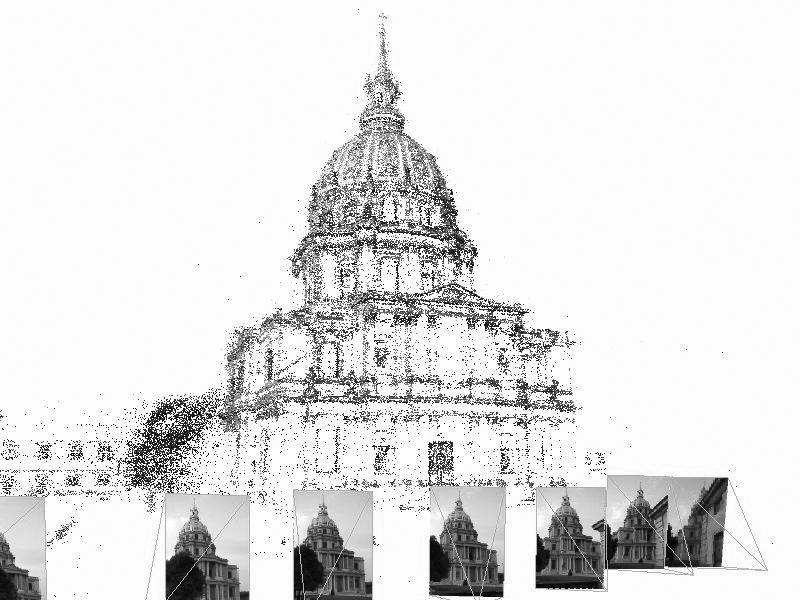
\includegraphics[scale=0.43]{images/eglise.jpg}
%\caption[Reconstrucci\'{o}n tridimensional de la \emph{Iglesia del Domo} en Paris]%
%{Con la t\'{e}cnica de \emph{estructura a partir del movimiento} es posible reconstruir estructuras como la \emph{Iglesia del Domo} en Paris utilizando \'{u}nicamente una secuencia de im\'{a}genes. Imagen de Carl Olsson \copyright \cite{olsson-etal-2011}.}
%\label{fig:Eglise}
%\end{figure}

%Una gran variedad de t\'{e}cnicas y algoritmos han sido creados para lidiar particularmente con problemas del campo de la visi\'{o}n artificial \cite{Cryer_Shah_1999,Faugeras_1993,Cyganek_Siebert_2009,Forsyth_Ponce_2002}. Por ejemplo, la detecci\'{o}n de caracter\'{i}sticas sobresalientes (del ingl\'{e}s \textit{feature detection}) permite encontrar informaci\'{o}n en im\'{a}genes la cual puede ser identificada posteriormente en otras im\'{a}genes de la misma escena. Al combinar este tipo de técnicas con

%Dos de las técnicas más desafiantes en el campo de la visión artificial son la

%La detección del flujo (del ingl\'{e}s \textit{optical flow})
%, \textit{visi\'{o}n estereosc\'{o}pica} (del ingl\'{e}s \textit{stereo vision}), \textit{estructura a partir del movimiento} (del ingl\'{e}s \textit{structure from motion}), permiten estimar la posici\'{o}n de puntos tridimensionales a partir de una secuencia de im\'{a}genes, los cuales pueden ser utilizados a su vez para determinar la geometr\'{i}a tridimensional del objeto o escena \cite{Faugeras_Luong_2001,Bay_Ess_Tuytelaars_Vangool_2008,Brostow_Shotton_Fauqueur_Cipolla_2008,Hartley_Zisserman_2003,Labatut_Pons_Keriven_2007,Cryer_Shah_1999}. Por ejemplo, la figura ~\ref{fig:Eglise} muestra una fase del proceso de reconstrucci\'{o}n tridimensional de la \emph{Iglesia del Domo} en Paris utilizando la t\'{e}cnica de \emph{estructura a partir del movimiento}, 85 c\'{a}maras y un total de 84792 puntos de la escena \cite{olsson-etal-2011}.


\subsection{¿Por qu\'{e} la visi\'{o}n artificial es tan dif\'{i}cil?}
En la visi\'{o}n artificial, una computadora recibe una matriz de n\'{u}meros que re\-pre\-senta la imagen capturada por la c\'{a}mara y nada m\'{a}s \cite{Shah_1983,Bradski_Kaehler_2008,Szeliski_2010,Cyganek_Siebert_2009}. No existen mecanismos empotrados que permitan reconocer patrones, no existen mecanismos automatizados que permitan controlar la apertura o el enfoque del lente, y finalmente, no existe un control cruzado de asociaciones hacia años de experiencia como en el caso de un ser humano.

\begin{figure}[H]
\centering
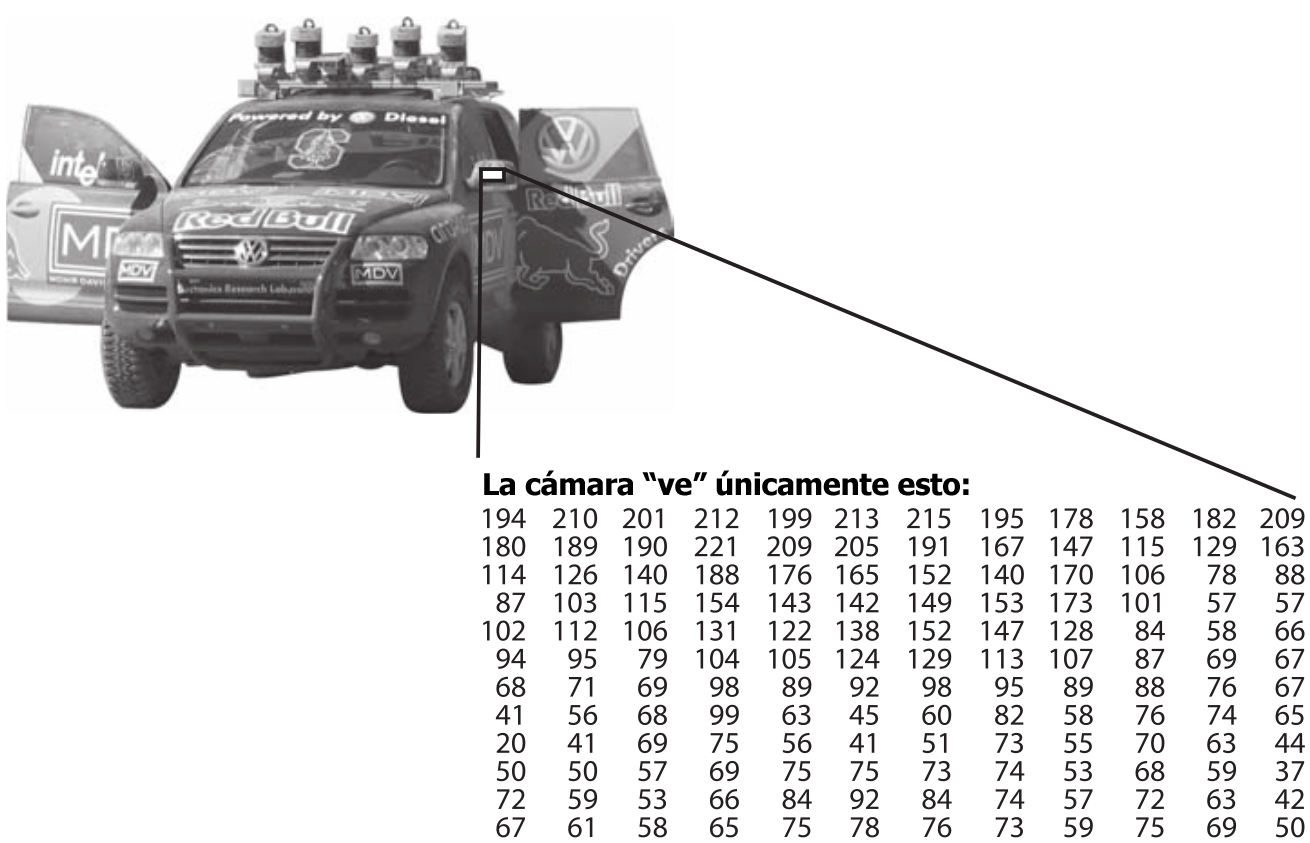
\includegraphics[width=1.0\textwidth]{images/fig1.png}
\caption[Lo que las computadoras ven en \emph{Visi\'{o}n Artificial}]%
{Para una computadora, el espejo retrovisor del carro es simplemente una matriz de n\'{u}meros. Imagen tomada del libro \emph{Learning OpenCV} \copyright \cite{Bradski_Kaehler_2008}.}
\label{fig:WhatComputersSee}
\end{figure}

Utilizando \'{u}nicamente la informaci\'{o}n brindada por una o m\'{a}s im\'{a}genes, se debe aplicar una serie de t\'{e}cnicas para determinar e interpretar su contenido y en el caso de procesos tridimensionales, recuperar la dimensi\'{o}n perdida (profundidad). La figura ~\ref{fig:WhatComputersSee} muestra la imagen de un autom\'{o}vil. En esa figura el ser humano es capaz de identificar f\'{a}cilmente el retrovisor del lado del conductor. Lo que una computadora \emph{ve} es simplemente una matriz de n\'{u}meros. Cada uno de los n\'{u}meros de esa matriz posee un amplio rango de \emph{ruido} y por lo tanto brinda muy poca informaci\'{o}n, pero esa matriz es todo lo que la computadora \emph{ve}.

\begin{figure}[H]
\centering
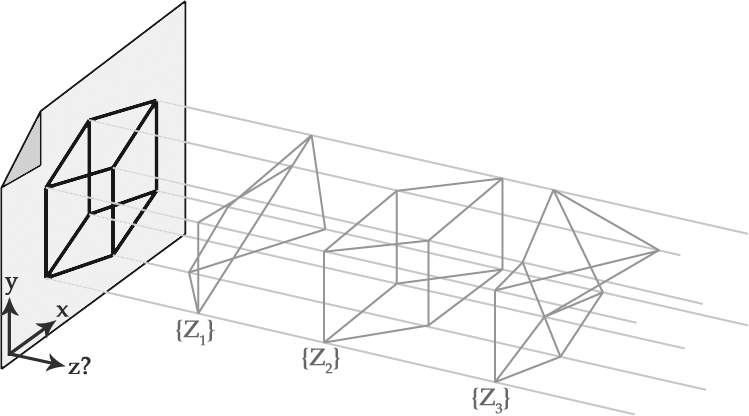
\includegraphics[width=1.0\textwidth]{images/2dto3dambiguity.png}
\caption[Problema de ambiguedad de una vista bidimensional (2D) de un mundo tridimensional (3D)]%
{Dada una vista bidimensional (2D) de un mundo tridimensional (3D), no existe una \'{u}nica o definitiva forma de reconstruir la señal 3D.}
\label{fig:2Dto3Dambiguity}
\end{figure}

Dada una vista bidimensional (2D) de un mundo tridimensional (3D), no existe una forma \'{u}nica o definitiva de reconstruir la señal 3D. De hecho el problema, es formalmente imposible de resolver \cite{Faugeras_Luong_2001,Bradski_Kaehler_2008,Hartley_Zisserman_2003}. La misma imagen 2D puede representar una colecci\'{o}n infinita de escenas 3D, a\'{u}n cuando los datos sean perfectos. En la figura ~\ref{fig:2Dto3Dambiguity} se muestra el problema de ambigüedad al reconstruir un cubo tridimensional a partir de una imagen bidimensional.

Los datos 2D se encuentran corruptos por ruido y distorsiones \cite{Freeman_Szeliski_2006,Thong_Sim_Phang_2001} provenientes del mundo real (clima, luz, reflecci\'{o}n, movimientos, sombras), de imperfecciones en el lente y construcci\'{o}n mec\'{a}nica de la c\'{a}mara, del ruido el\'{e}ctrico en el sensor u otros dispositivos electr\'{o}nicos y de la compresi\'{o}n de la imagen despu\'{e}s de ser capturada \cite{Szeliski_2010,Shah_1983,Faugeras_Luong_2001}.

A pesar de estas limitaciones, es posible utilizar conocimiento contextual adicional al diseñar un sistema pr\'{a}ctico, con tal de lidiar con los problemas impuestos por sensores visuales.

\section{Reconstrucci\'{o}n tridimensional}

\begin{figure}[H]
\centering
\subfloat[Reconstrucci\'{o}n pasiva de un objeto]{\label{fig:Pasive3DReconstruction}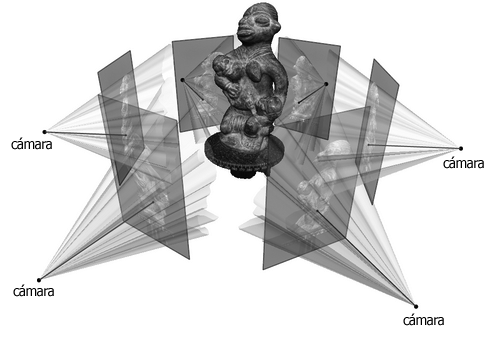
\includegraphics[width=0.5\textwidth]{images/pasive.png}}                
\subfloat[Reconstrucci\'{o}n activa de un objeto]{\label{fig:Active3DReconstruction}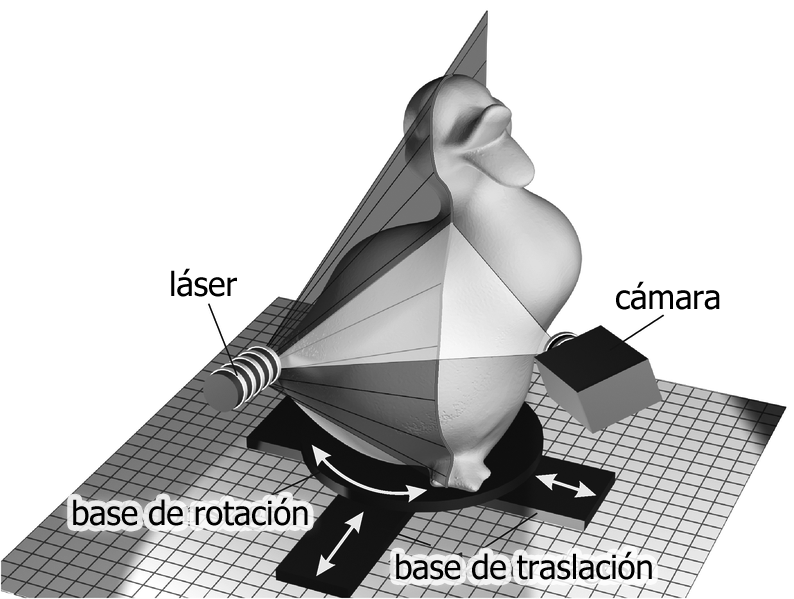
\includegraphics[width=0.5\textwidth]{images/active.png}}
\caption[Reconstrucci\'{o}n pasiva vs activa de un objeto tridimensional]%
{(a). Captura de im\'{a}genes durante el proceso pasivo de reconstrucci\'{o}n del objeto tridimensional. Imagen tomada de \url{http://carlos-hernandez.org/research.html} \copyright. (b). Proyecci\'{o}n de luz l\'{a}ser durante el proceso activo de re\-cons\-truc\-ci\'{o}n del objeto tridimensional. Imagen tomada de \url{http://en.wikipedia.org/wiki/File:LaserPrinciple.png} \copyright.}
\label{fig:3DReconstruction}
\end{figure}

La reconstrucci\'{o}n tridimensional es el proceso de capturar digitalmente la forma y apariencia de un objeto real. Este proceso puede ser realizado utilizando \emph{t\'{e}cnicas activas} o \emph{pasivas} \cite{Szeliski_2010,Forsyth_Ponce_2002,Cyganek_Siebert_2009}.

Al utilizar una \emph{t\'{e}cnica activa} de reconstrucci\'{o}n se interfiere activamente con el objeto. Generalmente, utiliza la proyecci\'{o}n de alg\'{u}n tipo de energ\'{i}a (luz l\'{a}ser o in\-fra\-rro\-ja) para lograr la reconstrucci\'{o}n. El c\'{a}lculo de la distancia tridimensional hacia los puntos del objeto se realiza por medio de la energ\'{i}a reflejada. Ejemplos de este tipo de t\'{e}cnica son c\'{a}maras in\-fra\-rro\-jas de profundidad, l\'{a}ser \emph{time-of-flight}, microondas o ultrasonido \cite{Rocchini_Cignoni_Montani_Pingi_Scopigno_2001,wiki:Janus_machine,Smisek_Jancosek_Pajdla_2011}. 

Por otro lado, al utilizar una \emph{t\'{e}cnica pasiva} de reconstrucci\'{o}n no se interfiere con el objeto. Generalmente, se utiliza un sensor con el cual se mide la radiaci\'{o}n reflejada o emitida por su superficie para determinar su estructura tridimensional. El sensor puede ser una c\'{a}mara fotogr\'{a}fica o de video sensible a la luz natural y los datos necesarios para la reconstrucci\'{o}n son el grupo de im\'{a}genes digitales (una o m\'{a}s) capturadas por \'{e}sta. El resultado final es una reconstrucci\'{o}n basada en im\'{a}genes \cite{Cyganek_Siebert_2009, Jahne_Haussecker_Geibler_1999, Faugeras_1992, Pollefeys_Gool_2002}. En la figura ~\ref{fig:3DReconstruction} se muestran las etapas de captura de im\'{a}genes (t\'{e}cnica pasiva) y proyecci\'{o}n de luz l\'{a}ser (t\'{e}cnica activa) para la reconstrucci\'{o}n de un objeto tridimensional.

Usualmente, un sistema completo de reconstrucci\'{o}n tridimensional se divide en tres grandes \'{a}reas: \emph{calibraci\'{o}n}, \emph{estimaci\'{o}n de la profundidad} y \emph{reconstrucci\'{o}n}.

\subsection{Calibraci\'{o}n}
Para determinar la profundidad a partir de una secuencia de im\'{a}genes es necesario realizar una calibraci\'{o}n de los puntos visuales de la c\'{a}mara y determinar sus par\'{a}metros extr\'{i}nsecos e intr\'{i}nsecos \cite{Jahne_Haussecker_Geibler_1999, Forsyth_Ponce_2002,Cyganek_Siebert_2009,Tsai_R_Y_1987}. En la figura ~\ref{fig:Calibration} se muestra una de las t\'{e}cnicas m\'{a}s populares de calibraci\'{o}n en la visi\'{o}n artificial utilizando un tablero de ajedrez.

\begin{figure}[H]
\centering
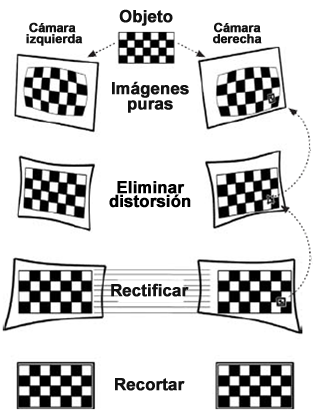
\includegraphics[width=0.4\textwidth]{images/calibration2.png}
\caption[T\'{e}cnica de calibraci\'{o}n utilizando un tablero de ajedrez]%
{La t\'{e}cnica de calibraci\'{o}n con tablero de ajedrez es una de las m\'{a}s po\-pu\-la\-res en la visi\'{o}n artificial. El proceso es necesario para revertir distorsiones en las im\'{a}genes causadas por la naturaleza mec\'{a}nica y electr\'{o}nica de las c\'{a}maras digitales. Imagen tomada de \url{http://meiyou.org/test2011/GSoC/} \copyright.}
\label{fig:Calibration}
\end{figure}

El proceso de calibraci\'{o}n permite determinar los par\'{a}metros necesarios para posteriormente corregir distorsiones en las im\'{a}genes generadas por el sistema de c\'{a}maras \cite{Bradski_Kaehler_2008,Shah_1983,Szeliski_2010, Tsai_R_Y_1987}. En la reconstrucci\'{o}n tridimensional se puede utilizar un aparejo con un par de c\'{a}maras (visi\'{o}n est\'{e}reo) calibradas \textit{a priori}. El problema de esta t\'{e}cnica est\'{a} en la dificultad de construir el aparejo y posicionar ambas c\'{a}maras con amplia precisi\'{o}n para obtener resultados aceptables en las im\'{a}genes estereosc\'{o}picas, limitando as\'{i} el uso pr\'{a}ctico del sistema \cite{Faugeras_Toscani_1986, Faugeras_Luong_2001, Faugeras_1993}. Por otro lado, es posible utilizar una secuencia de im\'{a}genes monosc\'{o}picas no calibradas generadas por una \'{u}nica c\'{a}mara y realizar la calibraci\'{o}n a partir de estos datos (auto-calibraci\'{o}n) \cite{Maybank_Faugeras_1992,Hartley_1993,Werner_Zisserman_2002,Hartley_Zisserman_2003}.

\subsection{Estimaci\'{o}n de la profundidad}
Es la etapa m\'{a}s compleja y desafiante del todo el proceso de reconstrucci\'{o}n tridimensional dado que hay que calcular la dimensi\'{o}n perdida (profundidad) a partir de im\'{a}genes bidimensionales. La estimaci\'{o}n de la profundidad se realiza utilizando \'{u}nicamente la informaci\'{o}n contenida en pares de im\'{a}genes es\-te\-reos\-c\'{o}pi\-cas, obtenidas por ejemplo por el sensor \emph{\ac{CCD}} de una c\'{a}mara.

Para estimar un modelo tridimensional de la escena se debe encontrar pareos entre pixeles de las im\'{a}genes y convertir sus posiciones 2D en posiciones 3D \cite{Cyganek_Siebert_2009, Szeliski_2010,Shah_1983}. A la distancia entre un pixel en una imagen y el mismo pixel en la otra imagen se le conoce como \emph{disparidad} \cite{Cyganek_Siebert_2009,Forsyth_Ponce_2002,Shah_1983}. Tal distancia es inversamente proporcional a la distancia de la profundidad y puede ser calculada por triangulaci\'{o}n.

Al resultado final de este proceso se le conoce como nube de puntos tridimensionales (del ingl\'{e}s \textit{point cloud}). En la figura ~\ref{fig:PointCloud} se muestra una nube de puntos calculados a partir de una secuencia de im\'{a}genes no calibradas.

\begin{figure}[H]
\centering
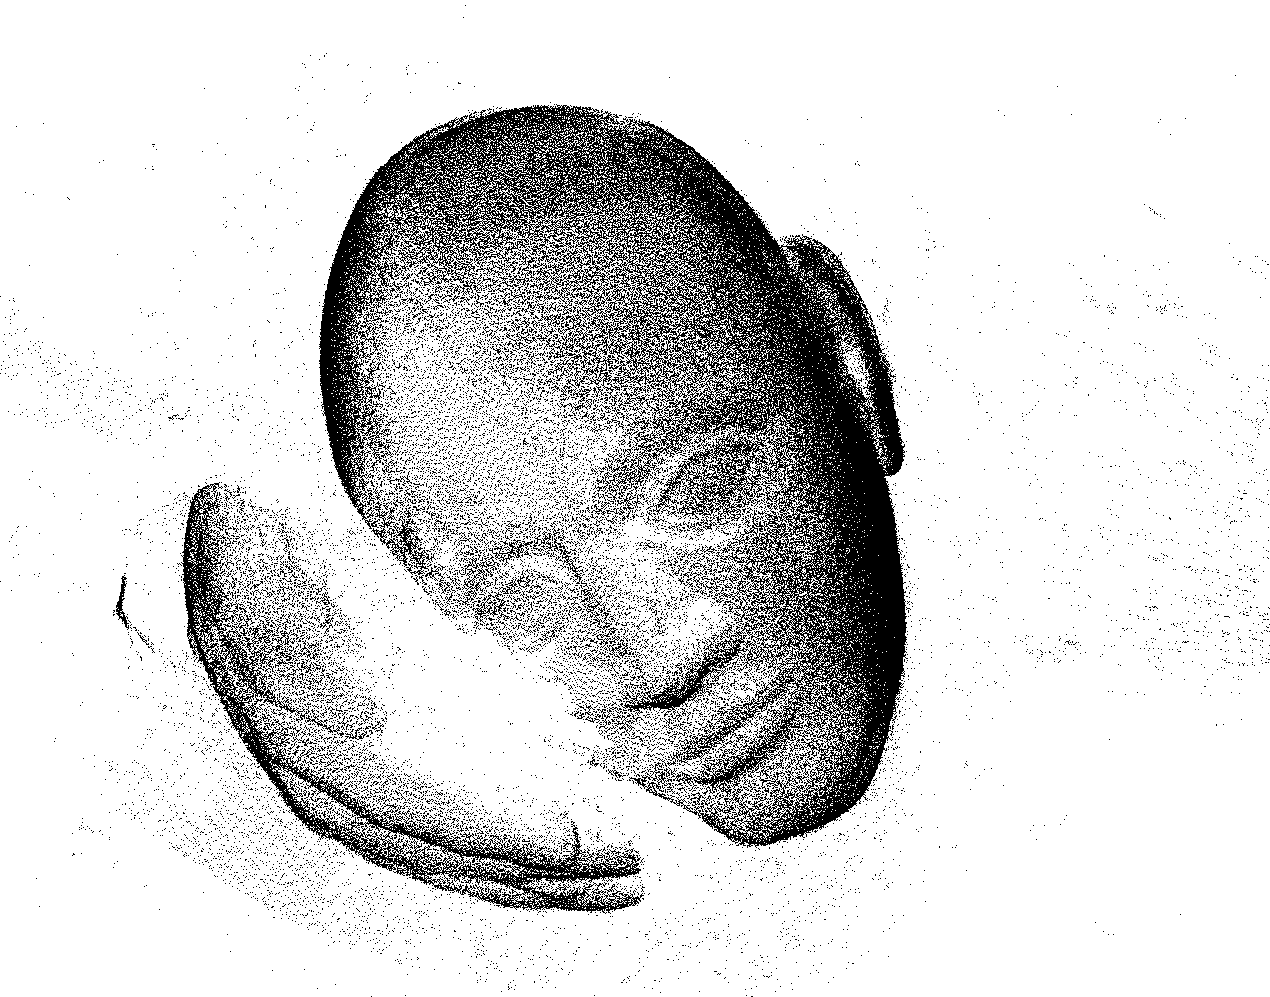
\includegraphics[width=0.6\textwidth]{images/point_cloud_b.png}
\caption[Nube de puntos calculada a partir de un objeto tridimensional]%
{Nube de puntos calculada a partir de una secuencia de im\'{a}genes no calibradas. Imagen tomada de \url{http://cmp.felk.cvut.cz/projects/is3d/} \copyright.}
\label{fig:PointCloud}
\end{figure}

\subsection{Reconstrucci\'{o}n}
La reconstrucci\'{o}n completa del objeto empieza con las diferentes nubes de puntos obtenidas en la fase anterior. Para modelar de forma completa (360\degree) un objeto se evaluan diferentes vistas para mejorar la geometr\'{i}a en reconstrucci\'{o}n (proceso conocido como \textbf{refinamiento}) \cite{Jahne_Haussecker_Geibler_1999,Cyganek_Siebert_2009}. Los grupos de puntos obtenidos se registran en un sistema de coordenadas consistente para obtener mapas de profundidad robustos (proceso conocido como \textbf{registro}). Finalmente, se convierten los diferentes mapas en una serie de modelos tridimensionales y se fusiona en un \'{u}nico modelo \cite{Cyganek_Siebert_2009, Bardsley_2008, Jahne_Haussecker_Geibler_1999, pan2009ProFORMA}. En la figura ~\ref{fig:3DModel} se muestra el resultado final de la reconstrucci\'{o}n completa del objeto.

\begin{figure}[H]
\centering
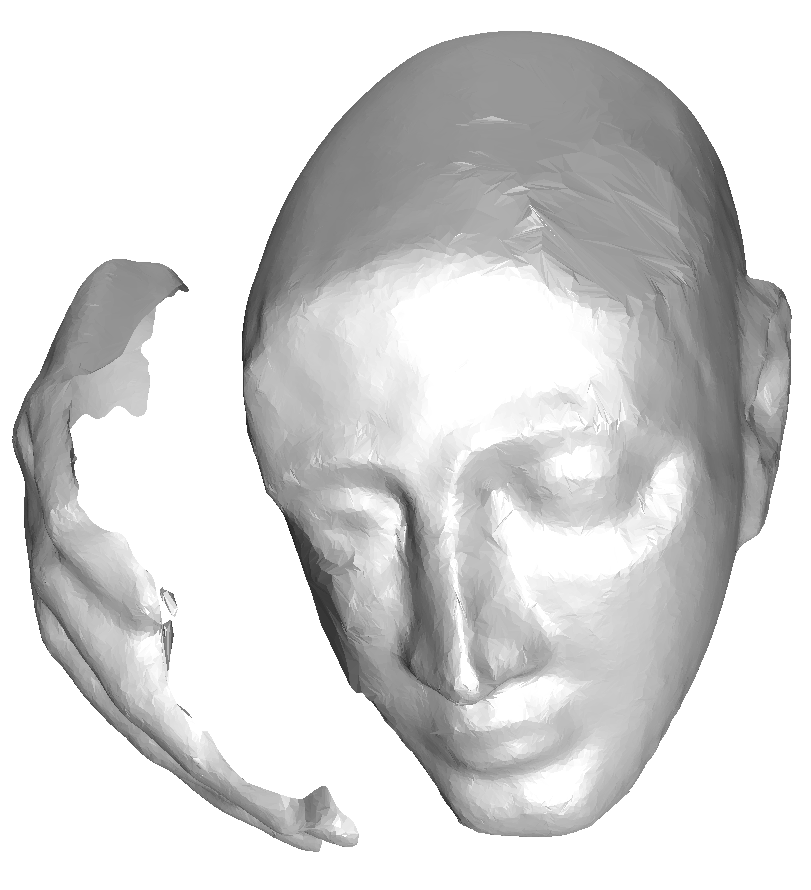
\includegraphics[width=0.45\textwidth]{images/Head-crust-faired-snap3.png}
\caption[Modelo de superficie tridimensional]%
{Modelo de superficie tridimensional obtenido a partir del proceso de refinamiento y fusi\'{o}n de los mapas de profundidad obtenidos a partir de las nubes de puntos. Imagen tomada de \url{http://cmp.felk.cvut.cz/projects/is3d/} \copyright.}
\label{fig:3DModel}
\end{figure}


\section{Trabajo relacionado}
Pan Q. et al. \cite{pan2009ProFORMA} proponen una t\'{e}cnica de reconstrucci\'{o}n basada en la utilizaci\'{o}n de descriptores para determinar la apariencia tridimensional del objeto. El problema de su t\'{e}cnica es que limita la reconstrucci\'{o}n a objetos con geometr\'{i}as muy simples (como cilindros y cubos), genera una cantidad excesiva de pol\'{i}gonos incluso en objetos simples y su reconstrucci\'{o}n es totalmente dispersa (pocos puntos). La t\'{e}cnica propuesta en este documento va m\'{a}s all\'{a} que reconstruir cilindros o cubos y pretende realizar una reconstrucci\'{o}n densa aprovechando todas las caracter\'{i}sticas f\'{i}sicas del objeto (forma, textura, color).

Kyle McDonald et al. \cite{wiki:Janus_machine} presentan un sistema activo que utiliza proyectores digitales, esc\'{a}neres y la t\'{e}cnica de luz estructurada para reconstruir tridimensionalmente la cabeza de la persona que se coloque frente al esc\'{a}ner. La utilizaci\'{o}n de equipo caro especializado como los proyectores y esc\'{a}neres es indeseable as\'{i} como el tiempo que tarda la construcci\'{o}n del modelo 3D.

Faugeras et al. \cite{Faugeras_1992} describen el tipo de informaci\'{o}n tridimensional que puede obtenerse al utilizar un aparejo binocular est\'{e}reo sin calibraci\'{o}n. Su t\'{e}cnica no toma en cuenta el tiempo de reconstrucci\'{o}n y se enfoca m\'{a}s en su resultado final.

Hassner et al. \cite{Hassner_Basri_2006} describen una t\'{e}cnica de reconstrucci\'{o}n utilizando una sola imagen bidimensional m\'{a}s una base de datos de objetos tridimensionales. La utilizaci\'{o}n de cualquier tipo de informaci\'{o}n \textit{a priori} para guiar la reconstrucci\'{o}n va en contra de lo propuesto en esta tesis.

Rocchini et al. \cite{Rocchini_Cignoni_Montani_Pingi_Scopigno_2001} proponen la creación de un esc\'{a}ner tridimensional de bajo costo basado en luz estructurada. La utilizaci\'{o}n de t\'{e}cnicas activas de reconstrucci\'{o}n, como es el caso de luz estructurada, necesita equipo especializado y costoso.


\section{Organizaci\'{o}n del documento}
El cap\'{i}tulo \ref{chap:descripcion} brinda una descripci\'{o}n general de la investigaci\'{o}n realizada. Se detalla la hip\'{o}tesis de la tesis en conjunto con el experimento utilizado para comprobar su validez. Luego se enumeran los objetivos de la tesis y finalmente, se brinda una secci\'{o}n de aportes, alcances y limitaciones de la t\'{e}cnica de reconstrucci\'{o}n r\'{a}pida propuesta.

En el cap\'{i}tulo \ref{chap:calibracion} se detalla todo el proceso de calibraci\'{o}n del experimento. Este cap\'{i}tulo es la base para lograr una buena reconstrucci\'{o}n tridimensional.

En el cap\'{i}tulo \ref{chap:profundidad} se describe el proceso de estimaci\'{o}n de la profundidad de los puntos tridimensionales del objeto a reconstruir el cual se basa en el algoritmo de triangulaci\'{o}n iterativo de m\'{i}nimos cuadrados.

En el cap\'{i}tulo \ref{chap:reconstruccion} se describe c\'{o}mo utilizar las matrices de la c\'{a}mara en conjunto con el algoritmo de triangulaci\'{o}n para reconstruir tridimensionalmente el objeto. Primero se brinda una descripci\'{o}n de c\'{o}mo realizar el proceso utilizando un par de vistas estereosc\'{o}picas y posteriormente, se muestra c\'{o}mo extenderlo a m\'{a}s de dos vistas.

En el cap\'{i}tulo \ref{chap:algoritmo} se describe el pseudoc\'{o}digo del algoritmo de reconstrucci\'{o}n propuesto en esta tesis y posteriormente, las principales diferencias con t\'{e}cnicas similares de reconstrucci\'{o}n.

%En el cap\'{i}tulo \ref{chap:algoritmo} se describe el pseudoc\'{o}digo del algoritmo de reconstrucci\'{o}n propuesto en esta tesis. Adicionalmente, se brinda su an\'{a}lisis de complejidad y finalmente, las principales diferencias con t\'{e}cnicas similares de reconstrucci\'{o}n.

En el cap\'{i}tulo \ref{chap:resultados} se muestran los resultados obtenidos durante las diferentes pruebas a las que fue sometida la t\'{e}cnica propuesta utilizando dos tipos distintos de c\'{a}maras.

En el cap\'{i}tulo \ref{chap:analisis} se detalla el an\'{a}lisis de los datos obtenidos durante la ejecuci\'{o}n de las diferentes pruebas del experimento.

Finalmente, en el cap\'{i}tulo \ref{chap:conclusiones} se presentan las conclusiones de la investigaci\'{o}n y el trabajo realizado. Luego, se detalla una secci\'{o}n relacionada con posibles mejoras y trabajo futuro.

%@TODO mejorar la descripcion de cada capitulo
%@TODO necesita conclusion del chapter???

\chapter{Descripci\'{o}n general de la investigaci\'{o}n}
\label{chap:descripcion}
\epigraph{Simplicity is prerequisite for reliability.}{Edsger W. Dijkstra}

En este cap\'{i}tulo se describe la investigaci\'{o}n realizada. Primero se brinda la hip\'{o}tesis, la cual propone que es posible reconstruir r\'{a}pidamente un objeto tridimensional del mundo real a partir de informaci\'{o}n contenida en im\'{a}genes capturadas con equipo barato, como es el caso de c\'{a}maras \textit{webcam}. Seguidamente, se detalla el experimento realizado para comprobar dicha hip\'{o}tesis. El experimento consta de una c\'{a}mara barata, una base giratoria de madera y la t\'{e}cnica de reconstrucci\'{o}n r\'{a}pida propuesta en esta tesis. Finalmente, se brinda una secci\'{o}n de aportes, alcances y limitaciones de dicha t\'{e}cnica.


\section{Hip\'{o}tesis}
La hip\'{o}tesis que defiende esta tesis dice que \textbf{es posible reconstruir r\'{a}pidamente un objeto tridimensional a partir de, \'{u}nicamente, la informaci\'{o}n contenida en una secuencia de im\'{a}genes que provienen de una c\'{a}mara convencional de bajo costo y utilizando una serie de t\'{e}cnicas del campo de la visi\'{o}n artificial.}


\section{Descripci\'{o}n general de la t\'{e}cnica}
La t\'{e}cnica presentada en esta tesis se basa en el mecanismo de estructura a partir del movimiento (del ingl\'{e}s \textit{structure from motion}), proceso que involucra estimar simult\'{a}neamente la geometr\'{i}a 3D (estructura) y la posici\'{o}n de la c\'{a}mara (movimiento) \cite{Ullman_1979,Szeliski_2010,Hartley_Zisserman_2003}. La t\'{e}cnica permite convertir r\'{a}pidamente pares de im\'{a}genes estereosc\'{o}picas bidimensionales de un objeto del mundo real en una representaci\'{o}n tridimensional de \'{e}ste, conocida como nube densa de puntos 3D.

La conversi\'{o}n de im\'{a}genes bidimensionales en una representaci\'{o}n tridimensional se inicia con una fase de calibraci\'{o}n de la c\'{a}mara, para determinar sus par\'{a}metros intr\'{i}nsecos y extr\'{i}nsecos. Posteriormente, se procede a aplicar una t\'{e}cnica pir\'{a}mide a las im\'{a}genes para reducir su procesamiento. Seguidamente, se realiza un rastreo denso y un pareo de pixeles entre cada par de im\'{a}genes estereosc\'{o}picas con tal de determinar su desplazamiento. Para lograr esto, se cre\'{o} un algoritmo de pareo denso basado en la detecci\'{o}n del flujo \'{o}ptico en lugar del tradicional pareo de caracter\'{i}sticas sobresalientes. Finalmente, se procede a determinar la profundidad calculando el movimiento entre c\'{a}maras (vistas) y luego triangulando los puntos del objeto utilizando el algoritmo iterativo de m\'{i}nimos cuadrados presentado en \cite{hartley1997triangulation}. En la figura ~\ref{fig:SystemOverview} se muestra el esquema general de la t\'{e}cnica r\'{a}pida de reconstrucci\'{o}n tridimensional.


\begin{figure}[H]
\centering
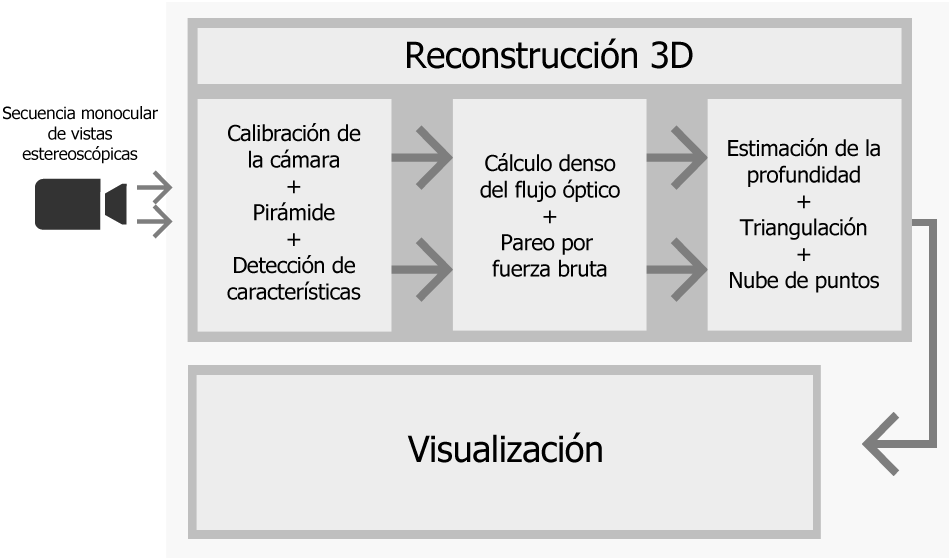
\includegraphics[width=1.0\textwidth]{images/systemoverview.png}
\caption[Esquema general de la t\'{e}cnica r\'{a}pida de reconstrucci\'{o}n tridimensional]%
{Esquema general de la t\'{e}cnica r\'{a}pida de reconstrucci\'{o}n tridimensional. Imagen creada por el autor de este documento.}
\label{fig:SystemOverview}
\end{figure}


Las fases de refinamiento, registro, \textit{meshing} y reconstrucci\'{o}n de la superficie no se contemplan en esta tesis pero pueden ser explorados en trabajo futuro.

\section{Descripci\'{o}n general del experimento}
Para el experimento se utilizaron dos c\'{a}maras tipo \textit{webcam} de bajo costo. La primera es una c\'{a}mara estereosc\'{o}pica con un sensor de baja definici\'{o}n conocida como \textit{Minoru 3D Webcam}. Creada en el 2009 por la compa\~n\'{i}a \textit{Promotion and Display Technology of Salford, Greater Manchester}, esta c\'{a}mara posee 2 sensores VGA de 640x480 y es capaz de capturar im\'{a}genes con resoluciones que van desde 320x240 hasta un m\'{a}ximo de 800x600. El monto invertido en la compra de la c\'{a}mara fue de \$21.42 en el a\~no 2011. En la figura ~\ref{fig:Camera1} se muestra esta c\'{a}mara.


\begin{figure}[H]
\centering
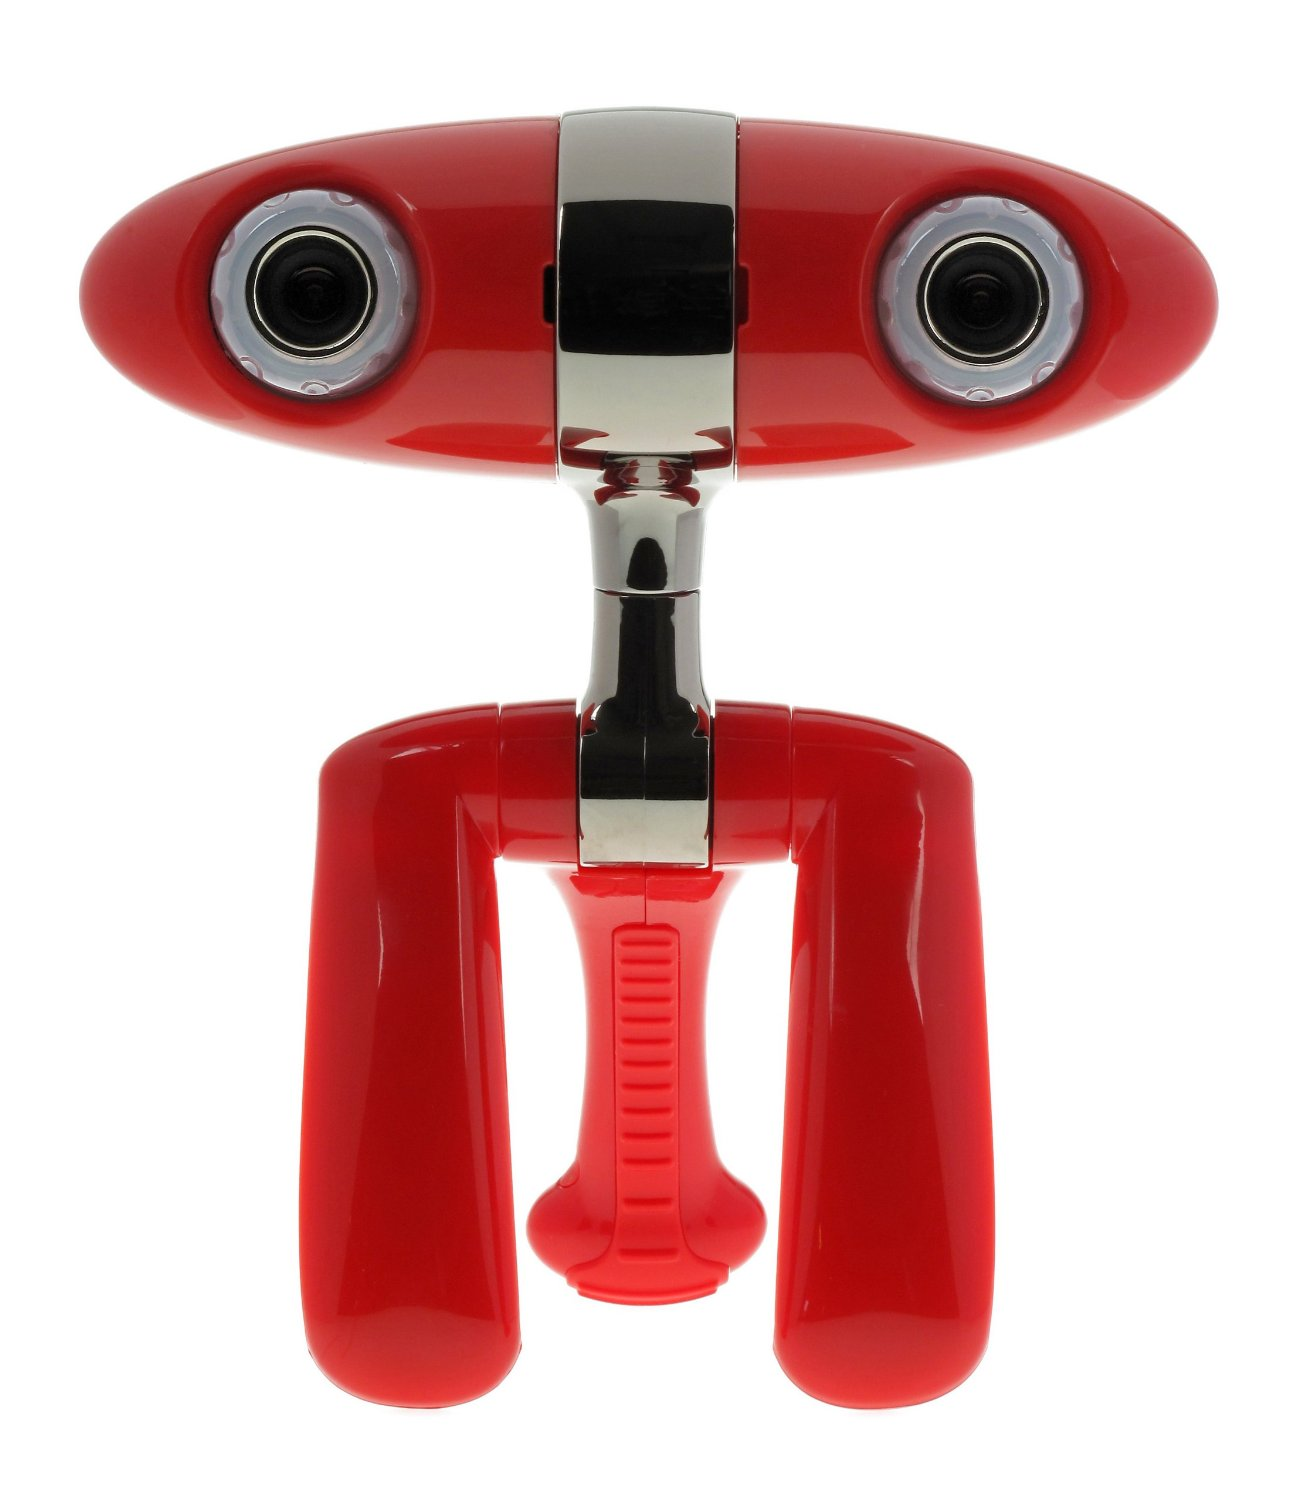
\includegraphics[width=0.7\textwidth]{images/camara1.jpg}
\caption[Minoru 3D Webcam]%
{La \textit{Minoru 3D Webcam} es una c\'{a}mara estereosc\'{o}pica de muy bajo costo que permite capturar im\'{a}genes 2D y 3D. M\'{a}s informaci\'{o}n en \url{http://www.minoru3d.com}.}
\label{fig:Camera1}
\end{figure}


La segunda es una c\'{a}mara con un lente de alta definici\'{o}n conocida como \textit{Logitech Webcam Pro C910}. Creada en el 2012 por la compa\~n\'{i}a \textit{Logitech}, esta c\'{a}mara posee un sensor de alta definici\'{o}n y un lente tipo \textit{Carl Zeiss\footnote{Carl Zeiss fue un alem\'{a}n que vivi\'{o} del a\~no 1816 al 1888, el cual fund\'{o} la compa\~n\'{i}a \textit{Carl Zeiss Jena} (ahora \textit{Carl Zeiss AG}). Para m\'{a}s informaci\'{o}n visitar \url{http://www.zeiss.com}} Tessar}\copyright el cual est\'{a} considerado como uno de los lentes de mayor calidad que existe en el mercado. Es capaz de capturar im\'{a}genes con resoluciones que van desde 160x120 hasta un m\'{a}ximo de 2592x1944. El monto invertido en la compra de la c\'{a}mara fue de \$70.62 en el a\~no 2011. En la figura ~\ref{fig:Camera2} se muestra esta c\'{a}mara.


\begin{figure}[H]
\centering
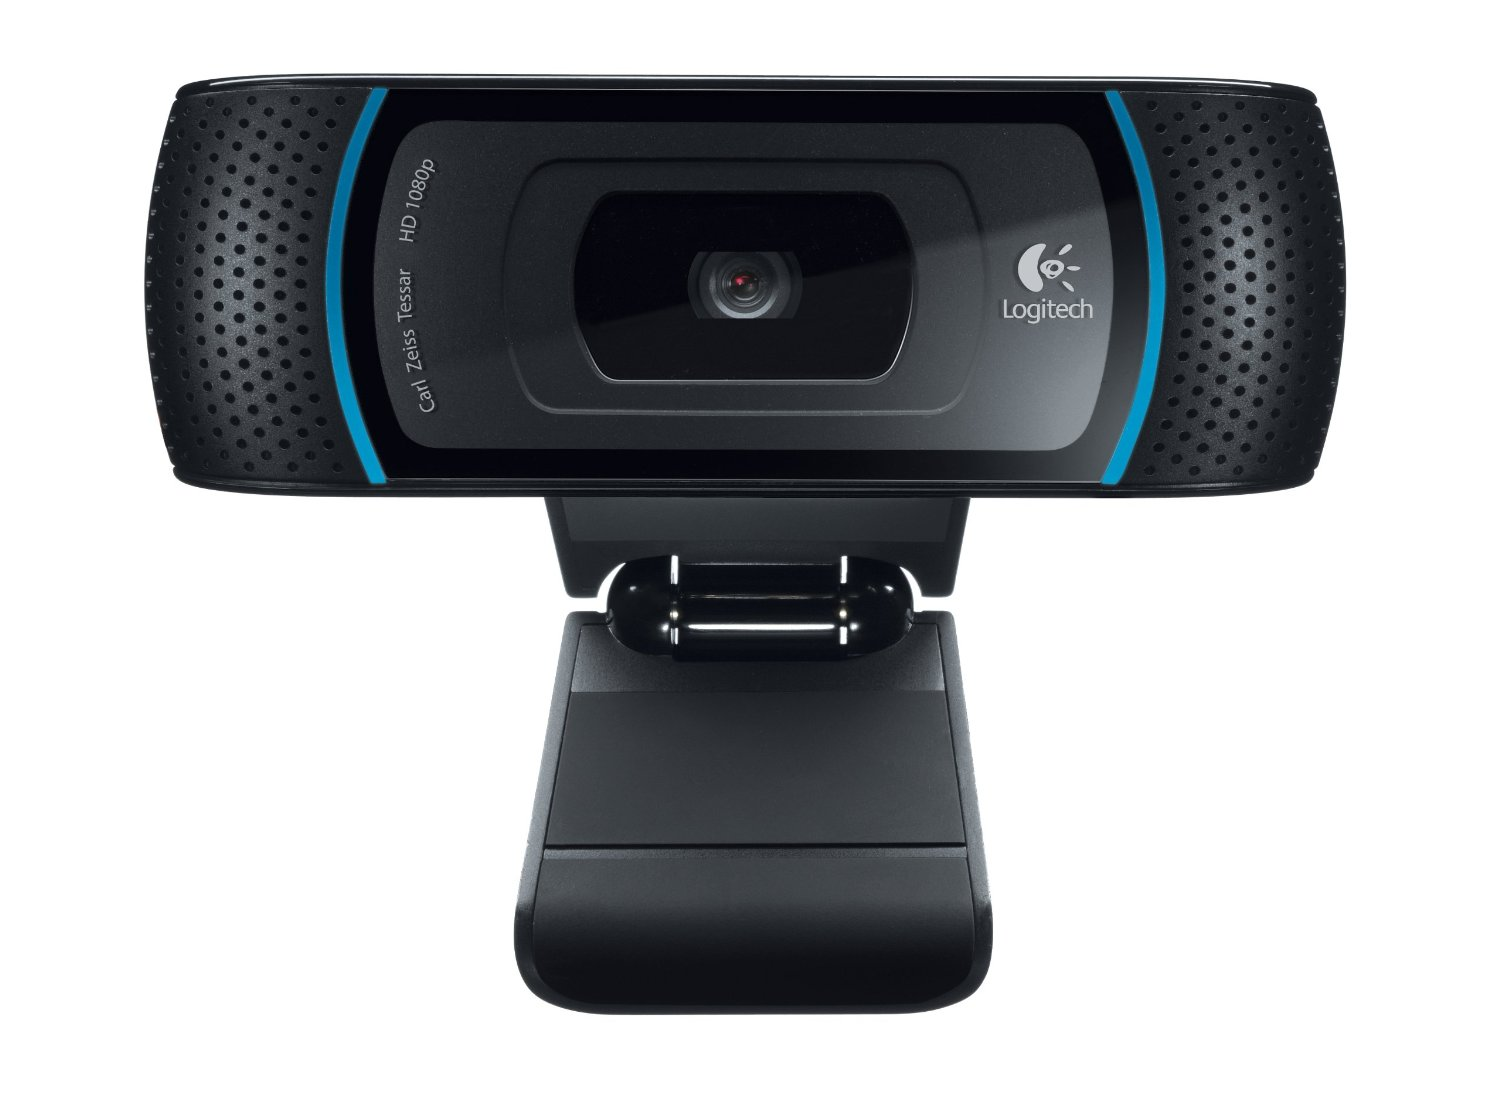
\includegraphics[width=1.0\textwidth]{images/camara2.jpg}
\caption[Logitech Webcam Pro C910]%
{La \textit{Logitech Webcam Pro C910} tiene un lente \textit{Carl Zeiss Tessar}\copyright y un sensor de alta definici\'{o}n. Más información en \url{http://www.logitech.com}.}
\label{fig:Camera2}
\end{figure}


Para realizar la reconstrucci\'{o}n, se posiciona una de las c\'{a}maras de forma fija a una distancia que permita observar gran parte o la totalidad del objeto a reconstruir. El objeto se posiciona sobre una base giratoria similar a la que se muestra en la figura ~\ref{fig:Base} y finalmente, se ejecuta el experimento utilizando una computadora personal. La luz afecta considerablemente la calidad de la reconstrucci\'{o}n, por lo que se recomienda que la base giratoria y el objeto se posicionen en un lugar con suficiente iluminaci\'{o}n.


\begin{figure}[H]
\centering
\includegraphics[width=1.0\textwidth]{images/base1.png}
\caption[Base giratoria]%
{Base giratoria hecha de una tapa de un envase de cocina, un rol de patineta, un portavasos de madera y un tornillo con tuerca. Monto total invertido en la construcci\'{o}n de la base: \$6.}
\label{fig:Base}
\end{figure}


No se hace ning\'{u}n tipo de suposici\'{o}n acerca de la geometr\'{i}a del objeto y no se conoce ning\'{u}n tipo de informaci\'{o}n del objeto \textit{a priori}. El \'{u}nico requerimiento particular de la t\'{e}cnica es la necesidad de que el objeto sea r\'{i}gido\footnote{Enti\'{e}ndase r\'{i}gido como un objeto cuya estructura geom\'{e}trica no var\'{i}a de una imagen a otra.} y que su textura no sea muy uniforme.


\begin{figure}[H]
\centering
\includegraphics[width=1.0\textwidth]{images/so.png}
\caption[Sistema completo utilizado para el experimento de la t\'{e}cnica r\'{a}pida de reconstrucci\'{o}n tridimensional]%
{Sistema completo utilizado para el experimento de la t\'{e}cnica r\'{a}pida de reconstrucci\'{o}n tridimensional. El sistema est\'{a} compuesto por una c\'{a}mara tipo \textit{webcam}, una base giratoria, el objeto a reconstruir y una computadora personal donde ejecutar los algoritmos.}
\label{fig:SO}
\end{figure}


Como se muestra en la figura ~\ref{fig:SO}, conforme el objeto va rotando frente a la c\'{a}mara, se toma una serie de vistas clave (del ingl\'{e}s \textit{keyframes}) para realizar la auto calibraci\'{o}n del sistema. Posteriormente, se procede con la fase r\'{a}pida de estimaci\'{o}n del movimiento en la cual se determinan los valores necesarios para reconstruir la posici\'{o}n y orientaci\'{o}n de la c\'{a}mara. Finalmente, se procede con la fase de recuperaci\'{o}n de la profundidad v\'{i}a el algoritmo iterativo de triangulaci\'{o}n. El resultado final es la representaci\'{o}n tridimensional del objeto en forma de una nube coloreada de puntos 3D. Todo el proceso toma unos cuantos segundos.




\section{Objetivo general}
\begin{itemize}
\item Desarrollar una t\'{e}cnica pasiva que permita la reconstrucci\'{o}n r\'{a}pida de un objeto tridimensional r\'{i}gido, utilizando una c\'{a}mara convencional de bajo costo m\'{a}s una serie de t\'{e}cnicas del campo de la visi\'{o}n artificial.
\end{itemize}

\section{Objetivos espec\'{i}ficos}
\begin{itemize*}
\item Desarrollar algoritmos para reconstruir el objeto 3D conforme la informaci\'{o}n de \'{e}ste es capturada.
\item Establecer la relaci\'{o}n matem\'{a}tica entre:
\subitem Resoluci\'{o}n de im\'{a}genes y tiempo de reconstrucci\'{o}n 3D.
\subitem Caracter\'{i}sticas f\'{i}sicas (tamaño, forma, color, textura) del objeto y tiempo de reconstrucci\'{o}n 3D.
\subitem Calibraci\'{o}n y calidad de la reconstrucci\'{o}n 3D.
\item Analizar y valorar t\'{e}cnicas actuales de reconstrucci\'{o}n 3D.
\item Mantener considerablemente bajo el costo global del sistema.
\end{itemize*}

\section{Aportes}
Este trabajo provee informaci\'{o}n, herramientas y metodolog\'{i}as relacionadas con la evaluaci\'{o}n de t\'{e}cnicas r\'{a}pidas de reconstrucci\'{o}n de objetos tridimensionales, las cuales pueden servir como base para trabajo futuro.

Tambi\'{e}n provee investigaci\'{o}n de calidad en el \'{a}rea de la visi\'{o}n artificial, con la esperanza de motivar futura investigaci\'{o}n en \'{e}sta. La visi\'{o}n artificial se ha vuelto relevante en Costa Rica en \'{a}reas como la seguridad vial e industrial.

Otro de los aportes de este trabajo es la correcci\'{o}n de problemas encontrados en algoritmos de la popular biblioteca de visi\'{o}n artificial \textit{OpenCV}\footnote{OpenCV es una biblioteca libre de visi\'{o}n artificial originalmente desarrollada por Intel. Desde que apareci\'{o} su primera versi\'{o}n alfa en el mes de enero de 1999, se ha utilizado en infinidad de aplicaciones. Para m\'{a}s informaci\'{o}n visitar \url{http://opencv.org}}. Durante el desarrollo de esta tesis se encontr\'{o} un problema con uno de los algoritmos de extracci\'{o}n de descriptores en el paquete \textit{Features2D} de los \textit{wrappers} de Java, el cual retornaba informaci\'{o}n incorrecta. Otro de los problemas encontrados fue en uno de los algoritmos de pareo por fuerza bruta del mismo paquete, el cual fallaba bajo ciertas condiciones. Para ambos problemas se realiz\'{o} el reporte correspondiente (\textit{bug report}) el cual fue aceptado por la comunidad y corregido posteriormente en la siguiente versi\'{o}n de la biblioteca.

\section{Alcances y limitaciones}
Se propuso la creaci\'{o}n de un prototipo funcional pr\'{a}ctico para realizar una reconstrucci\'{o}n r\'{a}pida de un objeto tridimensional r\'{i}gido. El prototipo completo debe estar compuesto \'{u}nicamente por una c\'{a}mara tipo \textit{webcam}, un computador de escritorio y los algoritmos necesarios para la reconstrucci\'{o}n.

Este trabajo no contempla los siguientes aspectos que podr\'{a}n ser explorados en trabajo futuro:
\begin{itemize*}
\item Reconstrucci\'{o}n de objetos con estructuras no r\'{i}gidas.
\item Reconstrucci\'{o}n de objetos con un ancho, alto y profundidad mayor a 30cm.
\item Reconstrucci\'{o}n de objetos con texturas muy uniformes.
\item Reconstrucci\'{o}n de objetos con estructuras muy irregulares.
\item Etapas posteriores a la triangulaci\'{o}n (refinamiento, registro, \textit{meshing}, reconstrucci\'{o}n de la superficie).
\item Utilizaci\'{o}n de equipo especializado (c\'{a}maras infrarrojas, de profundidad, proyectores, entre otros) o computadores de alto rendimiento.
\end{itemize*}



%@TODO describir el experimento completo, poner fotos del aparato, camaras y demas

%@TODO resumen del capitulo
\chapter{Calibraci\'{o}n}
\label{chap:calibracion}
\epigraph{On two occasions I have been asked, ‘If you put into the machine wrong figures, will the right answers come out?’  I am not able rightly to apprehend the kind of confusion of ideas that could provoke such a question.}{Charles Babbage}

En este cap\'{i}tulo se brinda una descripci\'{o}n del proceso utilizado para la calibraci\'{o}n del experimento. Primero se describe el modelo de c\'{a}mara utilizado en la t\'{e}cnica propuesta. Seguidamente, se detalla el algoritmo utilizado para obtener los par\'{a}metros intr\'{i}nsecos y extr\'{i}nsecos de la c\'{a}mara. Posteriormente, se detalla el algoritmo utilizado para calcular los elementos de rotaci\'{o}n y traslaci\'{o}n entre c\'{a}maras. Finalmente se describe el proceso para estimar la matriz fundamental y la matriz esencial de la c\'{a}mara. Cabe destacar que lograr una buena calibraci\'{o}n es de suma importancia dado que afecta considerablemente el resultado final de la reconstrucci\'{o}n.


\section{Modelo de c\'{a}mara}
Una c\'{a}mara es un mapeo entre el mundo 3D (espacio del objeto) y una imagen 2D. El modelo m\'{a}s b\'{a}sico de este mapeo es la c\'{a}mara \textit{\textbf{pinhole}} la cual no posee lente y puede ser construida utilizando una caja con una peque\~na abertura en uno de sus lados, como se muestra en la figura ~\ref{fig:Pinhole1}. La luz que rebota sobre la escena pasa \'{u}nicamente a trav\'{e}s de la abertura y proyecta una imagen invertida en la parte opuesta de la caja (plano proyectivo). 


\begin{figure}[H]
\centering
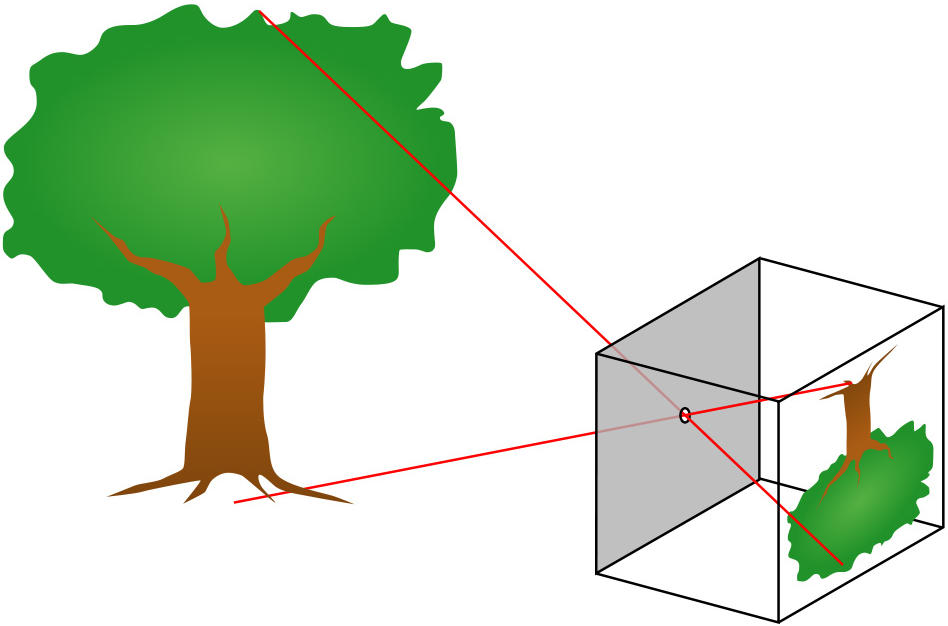
\includegraphics[width=0.8\textwidth]{images/pinhole1.png}
\caption[Modelo b\'{a}sico de c\'{a}mara \textit{pinhole}]%
{Los rayos de luz que rebotan sobre un objeto pasan a trav\'{e}s de un peque\~no agujero para formar una imagen invertida en el plano proyectivo. Imagen tomada del sitio \url{http://mediainfotain.blogspot.com/2010/08/types-of-camera.html} \copyright}
\label{fig:Pinhole1}
\end{figure}


De acuerdo con \cite{Hartley_Zisserman_2003,Faugeras_Luong_2001}, la geometr\'{i}a de esta c\'{a}mara asume que las coordenadas de la imagen son coordenadas Euclidianas con escalas iguales en ambas direcciones (\textit{x}, \textit{y}) como se muestra en la figura ~\ref{fig:Pinhole2}. Para el caso de c\'{a}maras \ac{CCD}, existe la posibilidad de tener pixeles no cuadrados. Si las coordenadas de la imagen se miden en pixeles, existe el efecto extra de introducir factores de escala desiguales en cada direcci\'{o}n. Afortunadamente, existe una variaci\'{o}n del modelo b\'{a}sico que permite determinar la transformaci\'{o}n entre coordenadas del mundo real a coordenadas de pixeles de la imagen.


\begin{figure}[H]
\centering
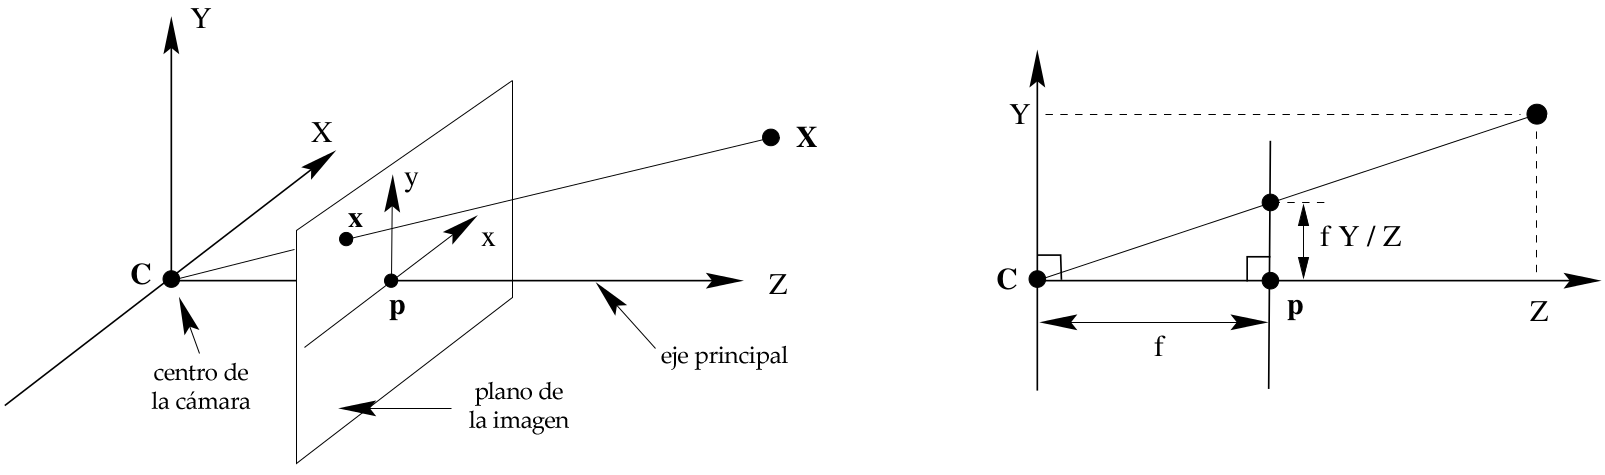
\includegraphics[width=1.0\textwidth]{images/pinhole.png}
\caption[Geometr\'{i}a de la c\'{a}mara \textit{pinhole}]%
{\textbf{C} es el centro de la c\'{a}mara y \textbf{p} el punto principal. El centro de la c\'{a}mara se posiciona justo en el origen de las coordenadas. N\'{o}tese que el plano de la imagen se posiciona frente al centro de la c\'{a}mara. Imagen tomada del libro \textit{Multiple View Geometry} de Richard Hartley y Andrew Zisserman \copyright \cite{Hartley_Zisserman_2003}.}
\label{fig:Pinhole2}
\end{figure}


Seg\'{u}n \cite{Szeliski_2010,Shah_1983}, la calibraci\'{o}n es el proceso de encontrar los valores \textit{verdaderos} de una c\'{a}mara que produce determinada fotograf\'{i}a o video. Usualmente, los par\'{a}metros de la c\'{a}mara son representados en la \textit{matriz de la c\'{a}mara} y los valores de distorsi\'{o}n son representados en la \textit{matriz de coeficientes de distorsi\'{o}n}. El algoritmo de calibraci\'{o}n del sistema de captura utilizado para la t\'{e}cnica de reconstrucci\'{o}n se basa en el modelo b\'{a}sico de c\'{a}mara \textit{pinhole} con proyecci\'{o}n perspectiva, como se indica en \cite{Hartley_Zisserman_2003}, en el cual la matriz de proyecci\'{o}n \textit{P} de la c\'{a}mara tiene la forma:

\begin{center}
\vspace{5 mm}
$
\textbf{\textit{P}} = \textbf{\textit{K}}[\textbf{\textit{R}}|\textbf{\textit{-Rt}}] con \textbf{\textit{K}} = 
\left[ {
\begin{array}{*{20}c}
   c_x & h_s & h_x  \\
   0   & c_y & h_y  \\
   0   & 0   & 1    \\
\end{array} 
} \right]
$
\vspace{5 mm}
\end{center}

donde \textit{\textbf{R}} indica la rotaci\'{o}n de la c\'{a}mara, \textit{\textbf{t}} es la posici\'{o}n del centro proyectivo en coordenadas del mundo real, \textit{\textbf{K}} contiene los par\'{a}metros internos de la c\'{a}mara: \textit{$c_x$} y \textit{$c_y$} son la longitud horizontal y vertical del foco (en pixeles), \textit{\textbf{h}} = $[h_x,h_y]^T$ es el punto principal de la imagen y \textit{$h_s$} es la medida de la inclinaci\'{o}n de la imagen (\textit{skew}). Afortunadamente, la matriz \textbf{\textit{K}} puede ser f\'{a}cilmente calculada utilizando la t\'{e}cnica de calibraci\'{o}n con tablero.

\section{Estimaci\'{o}n de K usando calibraci\'{o}n con tablero}
Por muchos a\~nos, la estimaci\'{o}n de los par\'{a}metros intr\'{i}nsecos y extr\'{i}nsecos de la c\'{a}mara ha sido un tema de gran inter\'{e}s para los investigadores del \'{a}rea de la visi\'{o}n artificial debido a que usualmente precede al proceso de reconstrucci\'{o}n de la profundidad \cite{Cyganek_Siebert_2009,Maybank_Faugeras_1992,Tsai_R_Y_1987}.

Una gran parte del inter\'{e}s ha sido dedicado al desarrollo de t\'{e}cnicas de calibraci\'{o}n r\'{a}pidas para c\'{a}maras simples, como es el caso de \cite{Zhang_camcal_2004} el cual propone un m\'{e}todo de calibraci\'{o}n de c\'{a}maras utilizando patrones gr\'{a}ficos.

La calibraci\'{o}n con tablero es una de las t\'{e}cnicas m\'{a}s populares en el \'{a}rea de la visi\'{o}n artificial por su relativa facilidad de implementaci\'{o}n y por su precisi\'{o}n en cuanto a los resultados \cite{Szeliski_2010, Tsai_R_Y_1987}. Para realizar la calibraci\'{o}n, se procede a presentar ante la c\'{a}mara un patr\'{o}n similar al de un tablero de ajedrez, con el cual es posible estimar con gran precisi\'{o}n la orientaci\'{o}n relativa y los par\'{a}metros intr\'{i}nsecos de la c\'{a}mara. El proceso calcula una m\'{e}trica Euclidiana con escala absoluta en el sistema de coordenadas de referencia de la calibraci\'{o}n \cite{Jahne_Haubecker_Ray_2002}, a partir de la cual es posible obtener la matriz de la c\'{a}mara \textbf{\textit{K}} y la matriz de coeficientes de distorsi\'{o}n. En la figura ~\ref{fig:ACalibration1} se muestra la ejecuci\'{o}n del algoritmo de calibraci\'{o}n con tablero utilizado durante el experimento.


\begin{figure}[H]
\centering
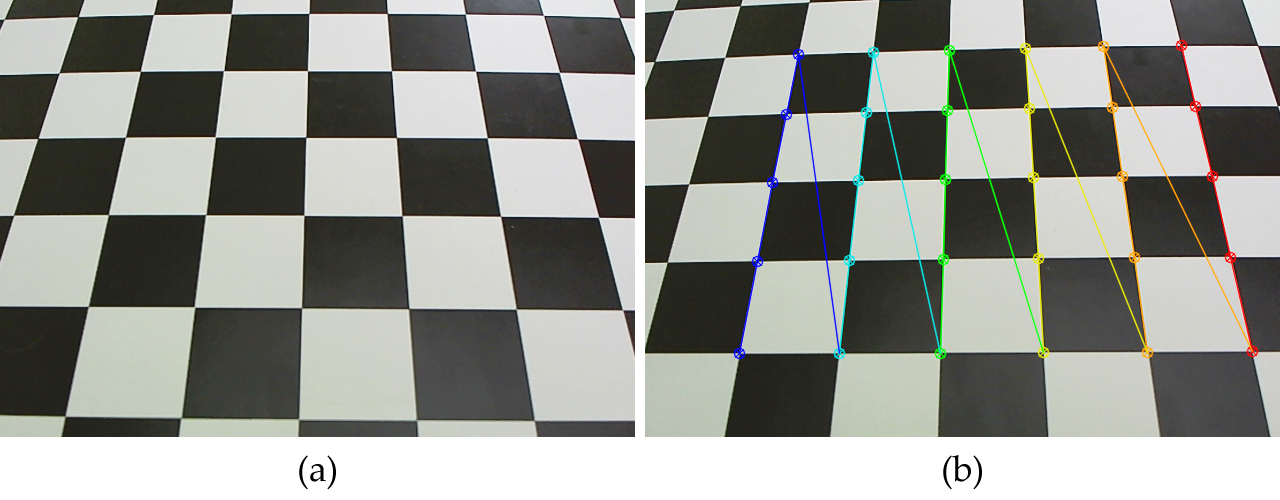
\includegraphics[width=1.0\textwidth]{images/acalibration0.png}
\caption[Calibraci\'{o}n usando tablero]%
{\textbf{(a)} Se presenta un patr\'{o}n de un tablero con un n\'{u}mero predeterminado de filas y columnas al algoritmo de calibraci\'{o}n. \textbf{(b)} El algoritmo calcula con gran precisi\'{o}n, a partir de los cuadros encontrados, la orientaci\'{o}n relativa as\'{i} como los valores intr\'{i}nsecos de la c\'{a}mara los cuales son necesarios para las siguientes etapas de la reconstrucci\'{o}n. Im\'{a}genes generadas por el autor de este documento.}
\label{fig:ACalibration1}
\end{figure}


\section{Estimaci\'{o}n del movimiento entre c\'{a}maras}
Una vez obtenida la matriz \textbf{\textit{K}} se procede a estimar el movimiento de la c\'{a}mara a partir de un par de im\'{a}genes estereosc\'{o}picas. Una c\'{a}mara\footnote{Con tal de simplificar la descripci\'{o}n de la t\'{e}cnica propuesta, se refiere a c\'{a}mara como la representaci\'{o}n de una vista (imagen) y no al aparato en s\'{i}.} tiene una posici\'{o}n en el espacio tridimensional y una direcci\'{o}n de la vista. Entre dos c\'{a}maras, existe un elemento de traslaci\'{o}n (matriz \textit{\textbf{t}}) y uno de rotaci\'{o}n (matriz \textit{\textbf{R}}) de la direcci\'{o}n de la vista, los cuales son necesarios para el proceso de la reconstrucci\'{o}n \cite{Faugeras_Luong_2001,Hartley_Zisserman_2003,Faugeras_1993}. En la figura ~\ref{fig:CameraMotion1} se muestra el movimiento de la c\'{a}mara entre pares de im\'{a}genes estereosc\'{o}picas.


\begin{figure}[H]
\centering
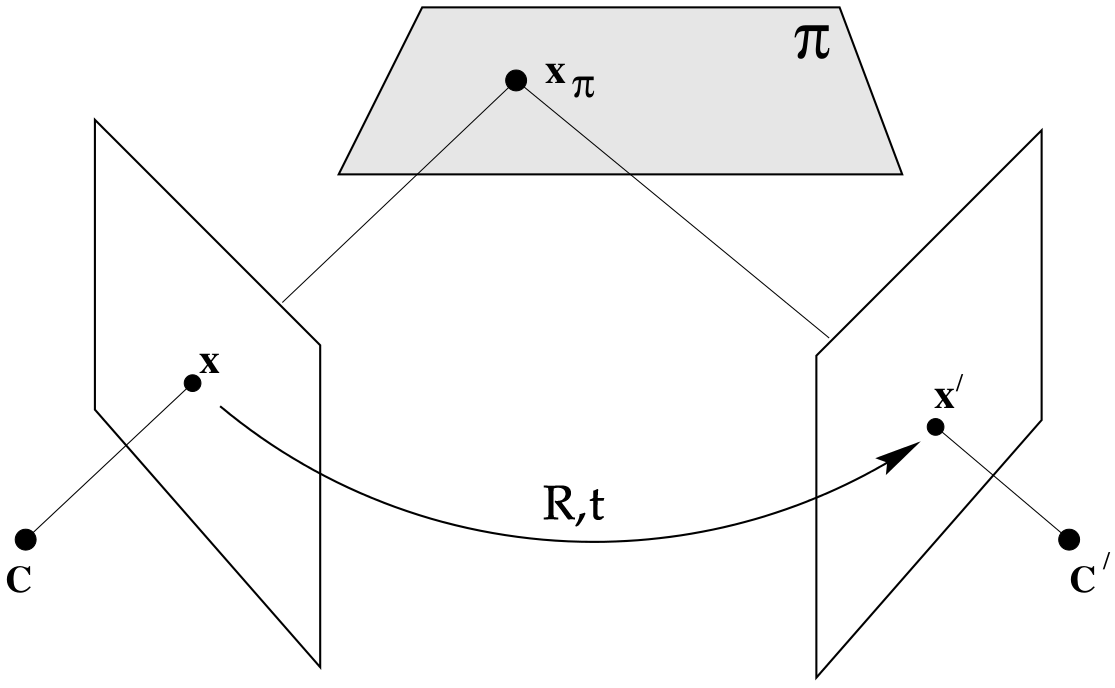
\includegraphics[width=1.0\textwidth]{images/camera-rt1.png}
\caption[Movimiento de c\'{a}mara entre pares de im\'{a}genes estereosc\'{o}picas]%
{La c\'{a}mara es indicada por su centro \textbf{C} en la primera posici\'{o}n en el espacio tridimensional y \textbf{C'} en la siguiente posici\'{o}n. Existe un elemento de rotaci\'{o}n \textbf{\textit{R}} y traslaci\'{o}n \textbf{\textit{t}} entre \textbf{C} y \textbf{C'} en pares de im\'{a}genes estereosc\'{o}picas. Imagen tomada del libro \textit{Multiple View Geometry} de Richard Hartley y Andrew Zisserman \copyright \cite{Hartley_Zisserman_2003}.}
\label{fig:CameraMotion1}
\end{figure}


En un aparejo est\'{e}reo (del ingl\'{e}s \textit{stereo rig}), el movimiento de traslaci\'{o}n y rotaci\'{o}n entre las c\'{a}maras se asume conocido \cite{Faugeras_Toscani_1986,Hartley_Zisserman_2003}. Tal es el caso de la c\'{a}mara estereosc\'{o}pica Minoru. La distancia entre sus dos c\'{a}maras puede ser calculada con precisi\'{o}n y as\'{i} evitar recalcularla para cada par de im\'{a}genes estereosc\'{o}picas tomadas con esta c\'{a}mara. Sin embargo, utilizar aparejos est\'{e}reo para realizar reconstrucci\'{o}n tridimensional tiene sus limitaciones pr\'{a}cticas y est\'{a} fuera del alcance de este trabajo. La t\'{e}cnica propuesta se basa en reconstrucci\'{o}n monocular (una c\'{a}mara). Es por esto que durante el experimento s\'{o}lo se utiliz\'{o} una de las dos c\'{a}maras de Minoru para la captura de las im\'{a}genes.

Dos im\'{a}genes (sean \textit{\textbf{I}} y \textit{\textbf{D}}) de un mismo objeto desde posiciones no muy diferentes en el espacio tridimensional (posiciones \textit{\textbf{a}} y \textit{\textbf{b}}) tomadas por una misma c\'{a}mara, son geom\'{e}tricamente equivalentes a tomar la imagen \textit{\textbf{I}} desde la posici\'{o}n \textit{\textbf{a}} con una c\'{a}mara y luego tomar la imagen \textit{\textbf{D}} desde la posici\'{o}n \textit{\textbf{b}} con una segunda c\'{a}mara. Esto significa que si se detecta una serie de puntos clave (del ingl\'{e}s \textit{keypoints}) en la imagen \textit{\textbf{I}} y luego se encuentran esos mismos puntos clave en la imagen \textit{\textbf{D}}, es posible determinar la traslaci\'{o}n \textit{t} y rotaci\'{o}n \textit{R} de las c\'{a}maras. Se puede determinar cu\'{a}nto y c\'{o}mo se ha movido un pixel entre una imagen y otra por medio de la estimaci\'{o}n de un mapa de movimiento (del ingl\'{e}s \textit{motion map}).

Cabe destacar que para la t\'{e}cnica propuesta es indiferente si procesa pares de im\'{a}genes provenientes de un aparejo est\'{e}reo o si procesa secuencias de im\'{a}genes provenientes de un sistema monocular como el utilizado.


\section{Mapa de movimiento}
Existen diferentes formas de obtener un mapa de movimiento. Algunas t\'{e}cnicas se basan en la detecci\'{o}n de l\'{i}neas \cite{Ding_Goshtasby_2001}, detecci\'{o}n de esquinas \cite{Harris_Stephens_1988}, detecci\'{o}n de \textit{blobs\footnote{En la visi\'{o}n artificial, la detecci\'{o}n de \textit{blobs} se refiere a los m\'{e}todos matem\'{a}ticos cuyo objetivo es detectar regiones en im\'{a}genes digitales que difieren en propiedades, tales como color o brillo, en comparaci\'{o}n con las \'{a}reas que se encuentran alderedor de esas regiones.}} \cite{Ming_Huadong_2007}, entre otras. 

Una de las t\'{e}cnicas m\'{a}s utilizadas en el campo de la visi\'{o}n artificial es el pareo entre caracter\'{i}sticas sobresalientes\footnote{Puntos clave y las caracter\'{i}sticas sobresalientes se refieren al mismo concepto.} (del ingl\'{e}s \textit{rich feature matching}). Lo que se hace es detectar en cada par de im\'{a}genes estereosc\'{o}picas un grupo de caracter\'{i}sticas sobresalientes con las cuales calcular descriptores invariantes para posteriormente realizar un pareo entre los grupos de cada imagen \cite{Shapiro_Stockman_2001,Szeliski_2010,Cyganek_Siebert_2009}.

Existe una cantidad considerable de algoritmos para la detecci\'{o}n de caracter\'{i}sticas sobresalientes, SIFT (del ingl\'{e}s \textit{scale-invariant feature transform}) \cite{Lowe_1999}, SURF (del ingl\'{e}s \textit{speeded up robust features}) \cite{Bay_Ess_Tuytelaars_Vangool_2008}, BRISK (del ingl\'{e}s \textit{binary robust invariant scalable keypoints}) \cite{Leutenegger_Chli_Siegwart_2011}, FAST (del ingl\'{e}s \textit{features from accelerated segment test}) \cite{Rosten_Drummond_2006}, HARRIS (por su autor Chris Harris) \cite{Harris_Stephens_1988} y muchos m\'{a}s. En la figura ~\ref{fig:PointDetection1} se muestran pruebas realizadas a cuatro de los algoritmos de detecci\'{o}n de caracter\'{i}sticas sobresalientes: \textit{BRISK}, \textit{DENSE}, \textit{SURF} y \textit{FAST} con pir\'{a}mide.


\begin{figure}[H]
\centering
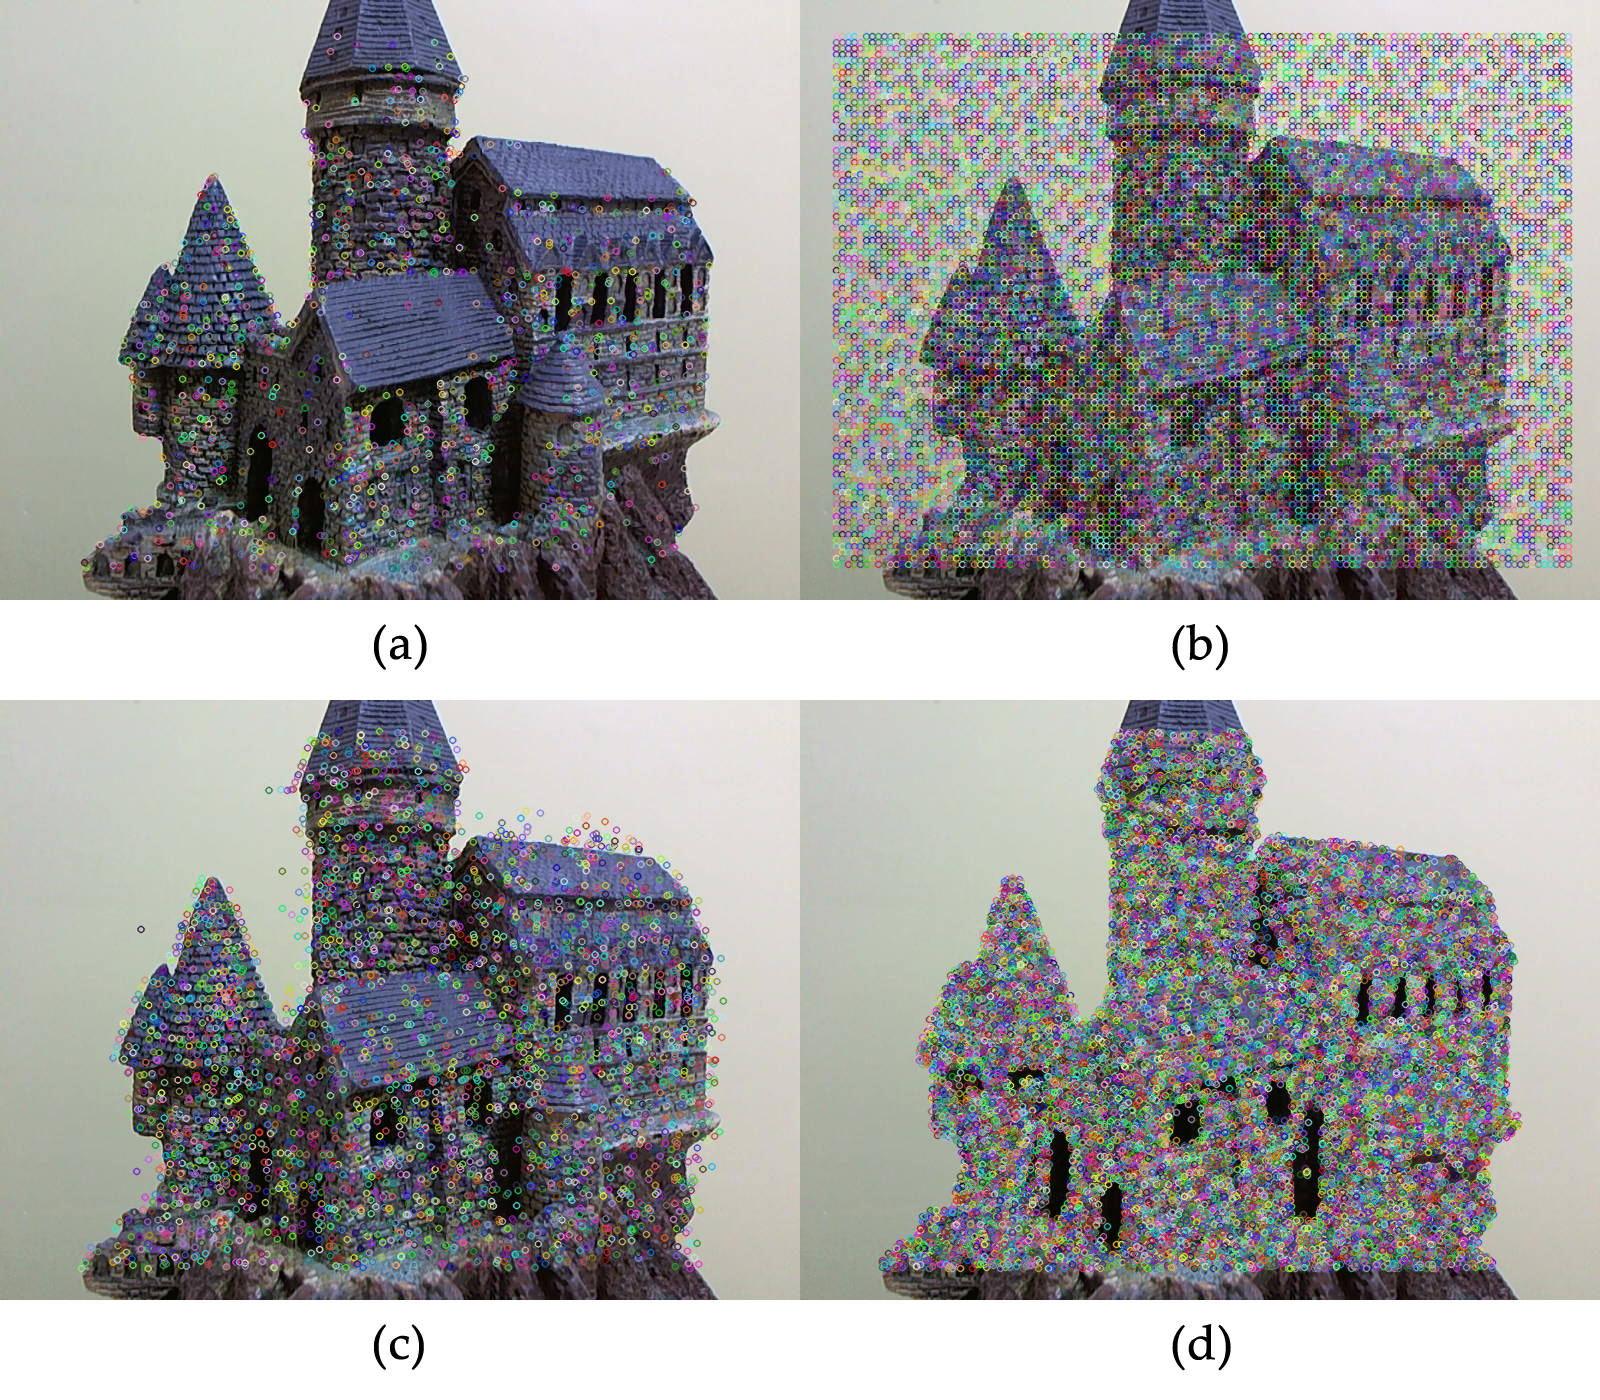
\includegraphics[width=1.0\textwidth]{images/pointdetection1.png}
\caption[Detecci\'{o}n de caracter\'{i}sticas sobresalientes usando BRISK, DENSE, SURF y FAST con pir\'{a}mide]%
{\textbf{(a)} \textit{BRISK} encontr\'{o} un total de 1176 puntos en la imagen. \textbf{(b)} \textit{DENSE} encontr\'{o} un total de 13400 puntos en la imagen. \textbf{(c)} \textit{SURF} encontr\'{o} un total de 3671 puntos en la imagen. \textbf{(d)} \textit{FAST} con pir\'{a}mide encontr\'{o} un total de 17296 puntos en la imagen. N\'{o}tese como \textit{SURF} y \textit{DENSE} detectaron puntos en \'{a}reas de la imagen en las cuales no existe nada sobresaliente mientras que \textit{FAST} con pir\'{a}mide no. La resoluci\'{o}n de la imagen es de 800x600 pixeles. Im\'{a}genes generadas por el autor de este documento.}
\label{fig:PointDetection1}
\end{figure}


De acuerdo con KITTI\footnote{KITTI es un proyecto del \textit{Karlsruhe Institute of Technology} y de \textit{Toyota Technological Institute at Chicago} el cual desarrolla evaluaciones para problemas del mundo real en el \'{a}rea de la visi\'{o}n artificial. Sitio web: \url{http://www.cvlibs.net/datasets/kitti}}, Middleburry\footnote{Middleburry College es una universidad privada ubicada en Middleburry, Vermont - USA. El sitio web \url{http://vision.middlebury.edu} se cre\'{o} como repositorio de evaluaciones y conjuntos de datos relacionados con la visi\'{o}n artificial.} y Computer Vision Talks \footnote{\textit{Computer Vision Talks} es un sitio dedicado a investigaciones en el \'{a}rea de la visi\'{o}n artificial. Sitio web: \url{http://computer-vision-talks.com/2011/01/comparison-of-the-opencvs-feature-detection-algorithms-2}}, \textit{FAST} con pir\'{a}mide, \textit{FAST} y \textit{SURF} son los algoritmos m\'{a}s r\'{a}pidos pero \textit{FAST} con pir\'{a}mide detecta una mayor cantidad de caracter\'{i}sticas, lo cual lo hace candidato adecuado para la t\'{e}cnica propuesta. En \cite{Tuytelaars_Mikolajczyk_2007} se detalla m\'{a}s a fondo c\'{o}mo funciona cada uno de los diferentes algoritmos.

Para la extracci\'{o}n de los descriptores se utiliz\'{o} ORB \cite{Rublee_Rabaud_Konolige_Bradski_2011} por su conocida eficiencia y rapidez en comparaci\'{o}n con algoritmos tradicionales como SIFT o SURF. Finalmente, se utiliz\'{o} un algoritmo de fuerza bruta \textit{BruteForce}, dado que es una de las formas m\'{a}s sencillas de comparar y hacer pareo entre caracter\'{i}sticas. B\'{a}sicamente, compara cada una de las caracter\'{i}sticas de un grupo contra las caracter\'{i}sticas del otro grupo y luego obtiene el mejor pareo entre ambos.

Sin embargo, despu\'{e}s de las diferentes pruebas realizadas se determin\'{o} que a pesar de que todo el proceso de detecci\'{o}n, extracci\'{o}n y pareo de caracter\'{i}sticas es relativamente r\'{a}pido, el mapa de movimiento resultante del pareo es muy disperso (pocos puntos) en la mayor\'{i}a de los casos. Esto provocar\'{i}a que el resultado final de la reconstrucci\'{o}n tridimensional tambi\'{e}n sea disperso. En la figura ~\ref{fig:FeatureMatching1} se muestran pruebas realizadas a tres de los algoritmos de pareo de caracter\'{i}sticas sobresalientes.


\begin{figure}[H]
\centering
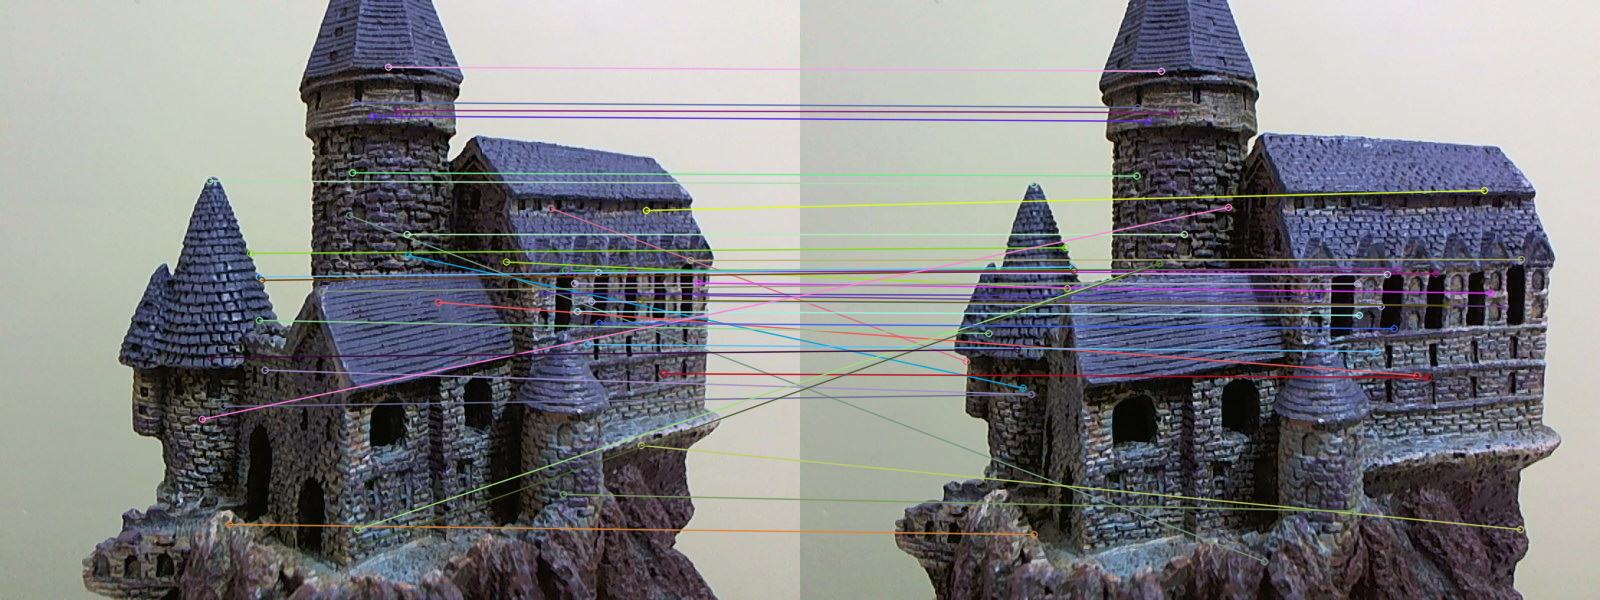
\includegraphics[width=1.0\textwidth]{images/briskmatches1.png}
(a)
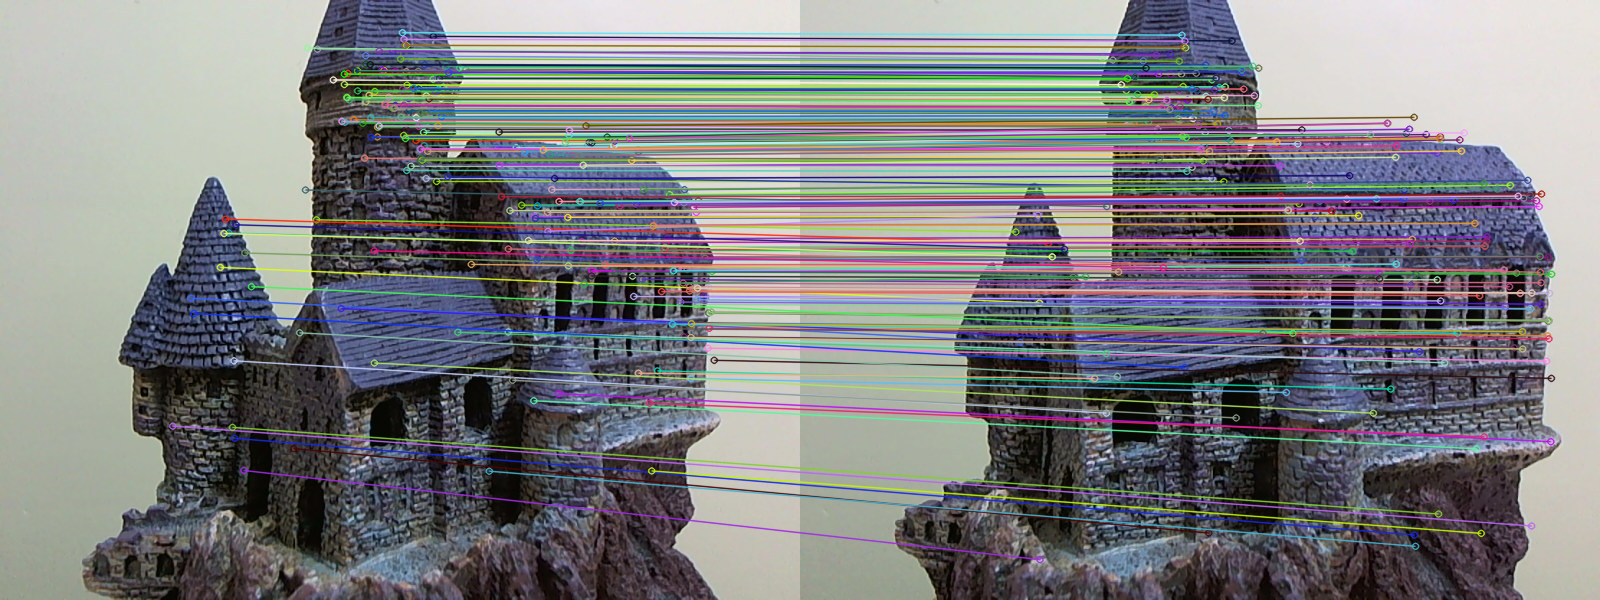
\includegraphics[width=1.0\textwidth]{images/surfmatches1.png}
(b)
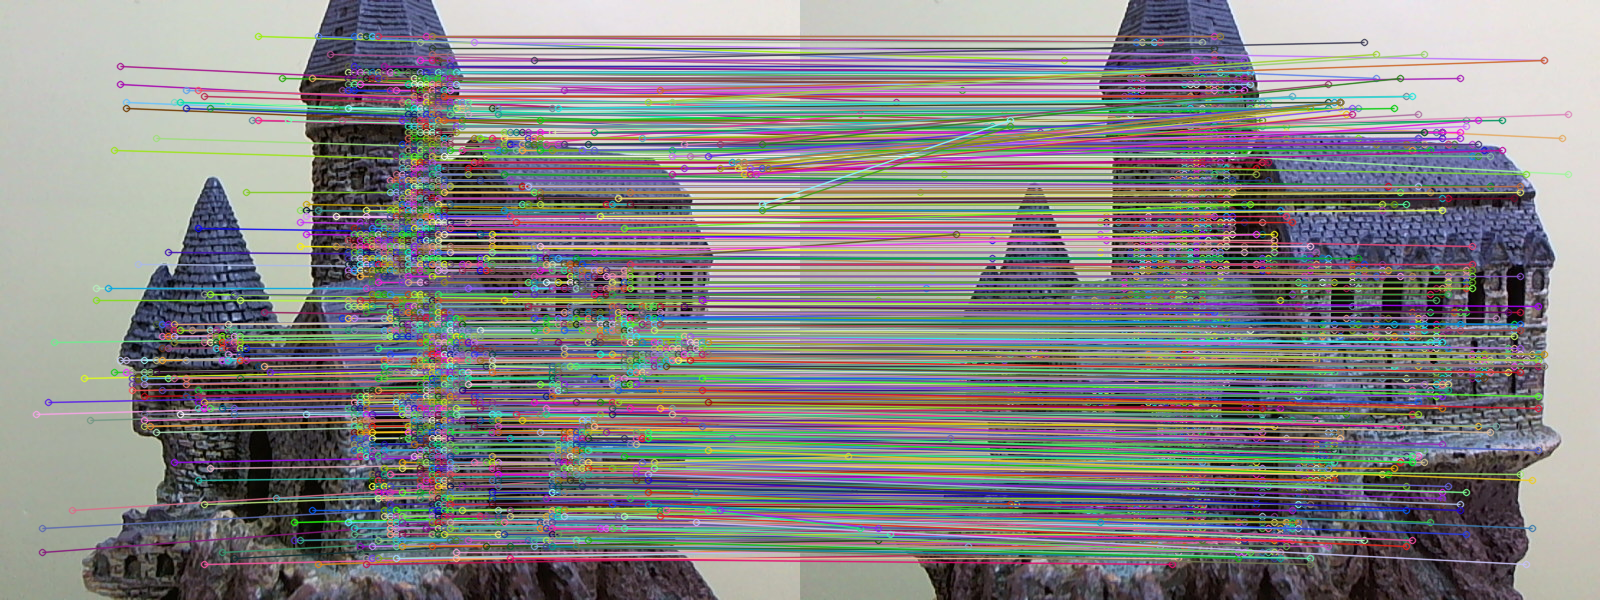
\includegraphics[width=1.0\textwidth]{images/densematches1.png}
(c)
\caption[Pareo de caracter\'{i}sticas y descriptores invariantes usando BRISK, SURF y DENSE]%
{\textbf{(a)} Pareo de caracter\'{i}sticas sobresalientes usando el algoritmo de BRISK. \textbf{(b)} Pareo de caracter\'{i}sticas sobresalientes usando el algoritmo de SURF. \textbf{(c)} Pareo de caracter\'{i}sticas sobresalientes usando el algoritmo de DENSE. N\'{o}tese, como el pareo entre el par de im\'{a}genes estereosc\'{o}picas es bastante disperso y en algunos casos incorrecto. Im\'{a}genes generadas por el autor de este documento.}
\label{fig:FeatureMatching1}
\end{figure}


Como se busca obtener una reconstrucci\'{o}n densa y no una dispersa, se opt\'{o} por desarrollar un algoritmo basado en la detecci\'{o}n del flujo \'{o}ptico (del ingl\'{e}s \textit{optical flow}) \cite{Szeliski_2010,Cyganek_Siebert_2009} en conjunto con una t\'{e}cnica pir\'{a}mide para el preprocesamiento de las im\'{a}genes. Generalmente, la detecci\'{o}n del flujo \'{o}ptico es costosa en tiempo y no apta para ser utilizada en reconstrucci\'{o}n tridimensional r\'{a}pida, dado que hay que rastrear todos y cada uno de los pixeles, pero el m\'{e}todo propuesto se basa en una reciente t\'{e}cnica lineal que es suficientemente r\'{a}pida para la reconstrucci\'{o}n y adicionalmente, permite generar mapas de movimiento densos.

\subsection{Preprocesamiento de im\'{a}genes usando pir\'{a}mide}
El concepto de im\'{a}genes pir\'{a}mide se define como una secuencia de copias de una imagen original en la cual la muestra de densidad y la resoluci\'{o}n han sido disminuidas a pasos regulares, usualmente por un factor de 2 en cada coordenada \cite{Adelson_Anderson_Bergen_Burt_Ogden_1984}. Se busca reducir la cantidad de informaci\'{o}n contenida en la imagen sin que se degrade su calidad durante el procesamiento.

Dos de las t\'{e}cnicas m\'{a}s utilizadas de im\'{a}genes pir\'{a}mide son pir\'{a}mide \textit{Gaussian} y pir\'{a}mide \textit{Laplacian}. La t\'{e}cnica de pir\'{a}mide Gaussian se utiliza para reducir la informaci\'{o}n contenida en las im\'{a}genes mientras que la t\'{e}cnica pir\'{a}mide Laplacian se utiliza para reconstruir una imagen interpolada a partir de una imagen inferior de la pir\'{a}mide (con menor resoluci\'{o}n) \cite{Burt198120,burt_adelson_1095851}.


\begin{figure}[H]
\centering
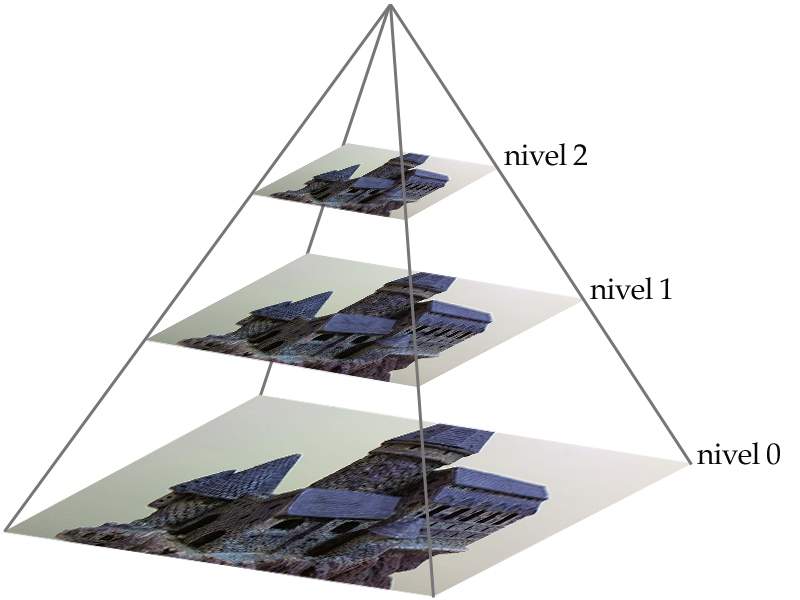
\includegraphics[width=0.75\textwidth]{images/pyramid.png}
\caption[Preprocesamiento de im\'{a}genes usando pir\'{a}mide]%
{En el nivel 0 se encuentra la imagen original con una resoluci\'{o}n de 800x600 lo cual equivale a una cantidad de 480000 pixeles. El nivel 1 muestra la misma imagen reducida a 640x480 con una cantidad de 307200 pixeles y finalmente, la imagen en el nivel 2 con una resoluci\'{o}n de 512x384 equivalente a una cantidad de 196608 pixeles. La reducci\'{o}n en la cantidad de pixeles entre la imagen original y la imagen en el nivel 2 es de un 40.96\%. Imagen generada por el autor de este documento.}
\label{fig:Pyramid}
\end{figure}


Para la t\'{e}cnica propuesta, cada imagen es preprocesada utilizando pir\'{a}mide Gaussian con un factor 2 para reducir la cantidad de informaci\'{o}n que se procesar\'{a} durante la fase de detecci\'{o}n del flujo \'{o}ptico\footnote{La escogencia del factor se realiz\'{o} de forma emp\'{i}rica basada en las diferentes investigaciones y pruebas realizadas pero la t\'{e}cnica no se encuentra limitada por este factor.}. Esto permite mantener bajo el tiempo global de la reconstrucci\'{o}n cuando se utilicen im\'{a}genes de gran resoluci\'{o}n sin afectar considerablemente su calidad. En la figura ~\ref{fig:Pyramid} se muestran un ejemplo de la t\'{e}cnica pir\'{a}mide Gaussian aplicada a una de las im\'{a}genes capturadas durante el experimento.


\subsection{R\'{a}pida detecci\'{o}n del flujo \'{o}ptico}
El primero en introducir este concepto fue el psic\'{o}logo James J. Gibson en 1940 y lo describe como \textit{el est\'{i}mulo visual dotado a los animales que se mueven a trav\'{e}s de la Tierra} \cite{Gibson_1950}. En el \'{a}rea de la visi\'{o}n artificial, el flujo \'{o}ptico trabaja rastreando todos y cada uno de los pixeles de la primera imagen en la segunda imagen, asumiendo que ambas im\'{a}genes son parte de una secuencia y que se encuentran relativamente cerca una de la otra, con el supuesto de que cada pixel puede moverse solamente dentro de cierta \textit{ventana} en la cual se realizar\'{a} la b\'{u}squeda \cite{Gibson_1950,Shapiro_Stockman_2001,Szeliski_2010,Cyganek_Siebert_2009}.

Entre los algoritmos m\'{a}s populares para la detecci\'{o}n densa\footnote{En este contexto, densa significa que se busca el movimiento de todos y cada uno de los pixeles de la imagen.} del flujo \'{o}ptico se encuentran el de \textit{Lucas-Kanade} \cite{Lucas_Kanade_1981} y m\'{a}s recientemente el de \textit{Gunnar Farnebäck} \cite{Farneback_2003}. Usualmente, la detecci\'{o}n densa es costosa en tiempo pero afortunadamente ambos algoritmos son lo suficientemente r\'{a}pidos para ser utilizados en la reconstrucci\'{o}n tridimensional y han sido implementados en una gran variedad de bibliotecas. De acuerdo con KITTI y Middleburry, el algoritmo de Farnebäck es m\'{a}s r\'{a}pido y posee una menor tasa de error\footnote{V\'{e}ase \url{http://www.cvlibs.net/datasets/kitti/eval_stereo_flow.php}}. En la figura ~\ref{fig:OpticalFlow1} se muestra el resultado de una de las pruebas de detecci\'{o}n del flujo \'{o}ptico utilizando el algoritmo de Lucas-Kanade y el de Farnebäck.


\begin{figure}[H]
\centering
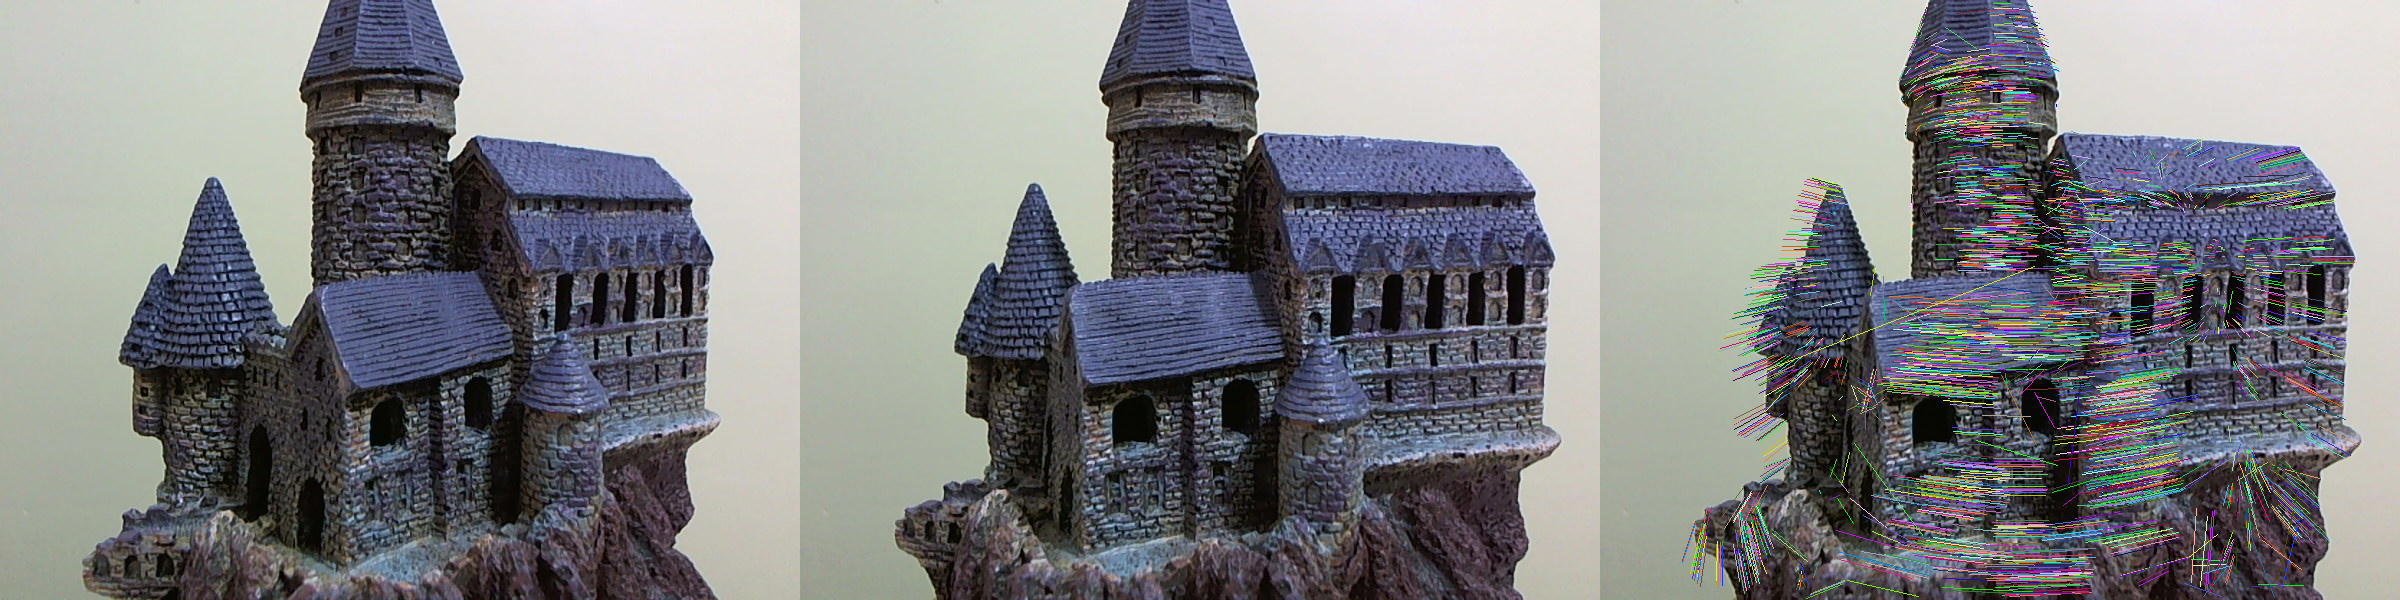
\includegraphics[width=1.0\textwidth]{images/oflucaskanade1.png}
(a)
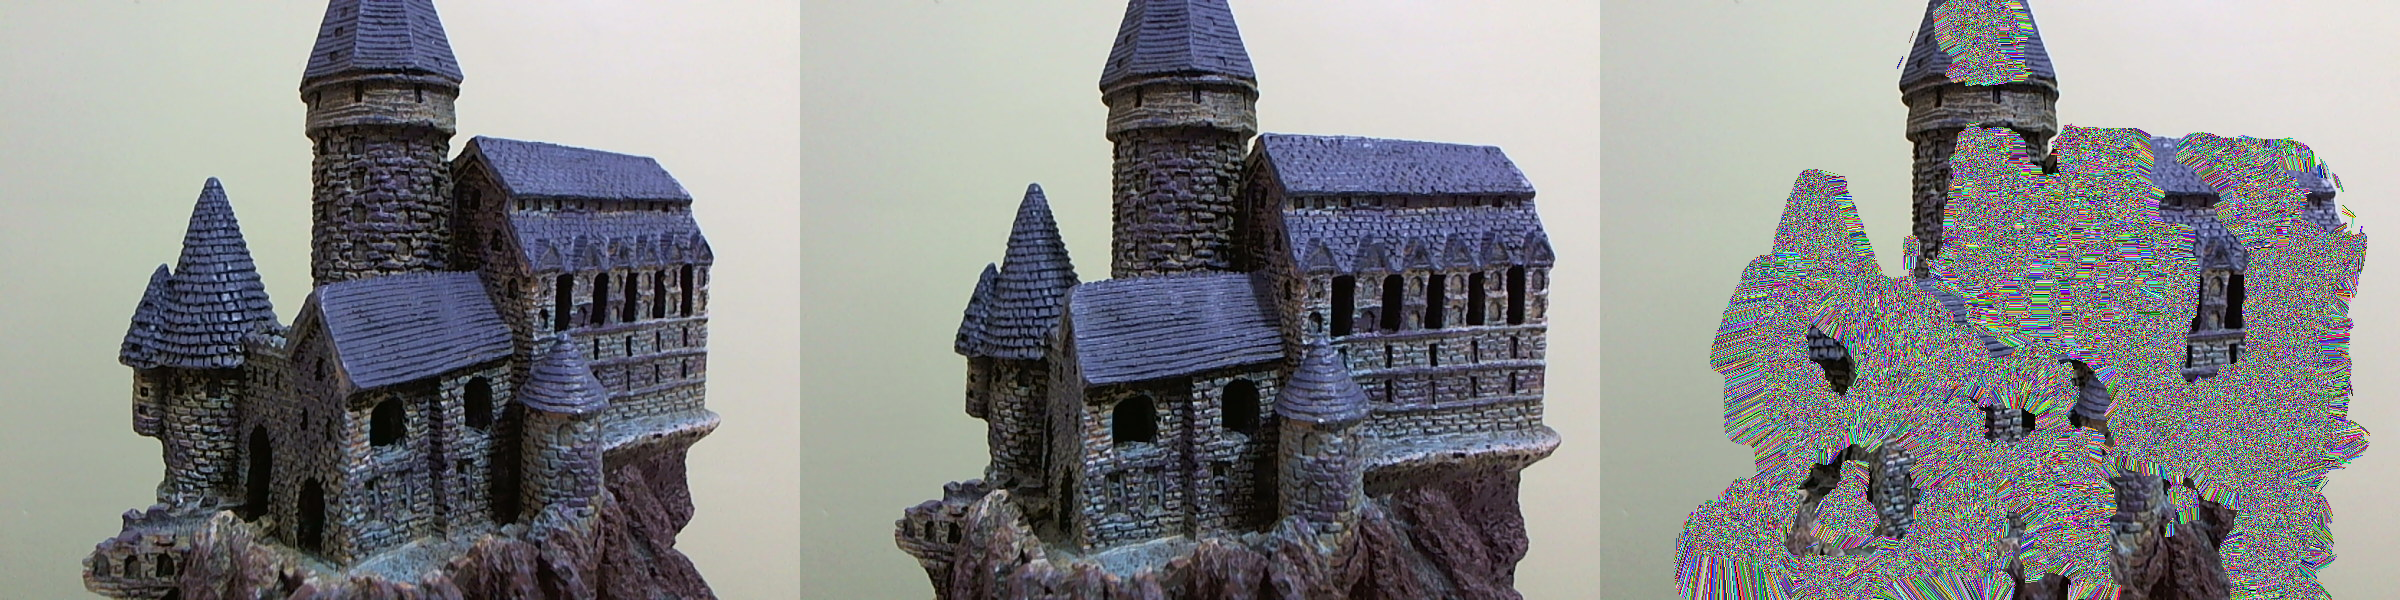
\includegraphics[width=1.0\textwidth]{images/offarneback1.png}
(b)
\caption[Detecci\'{o}n del flujo \'{o}ptico]%
{\textbf{(a)} Detecci\'{o}n densa del flujo \'{o}ptico utilizando el algoritmo de Lucas-Kanade. \textbf{(b)} Detecci\'{o}n densa del flujo \'{o}ptico utilizando el algoritmo de Gunnar Farnebäck. N\'{o}tese la considerable diferencia entre el flujo detectado por Lucas-Kanade vs. Farnebäck. Ambas t\'{e}cnicas est\'{a}n entre las m\'{a}s populares y ha sido implementadas en una gran variedad de bibliotecas de visi\'{o}n artificial. Im\'{a}genes generadas por el autor de este documento.}
\label{fig:OpticalFlow1}
\end{figure}


Farnebäck permite generar el mapa denso de movimiento requerido para la calibraci\'{o}n. Sin embargo, pruebas realizadas tanto al algoritmo de Lucas-Kanade como el de Farnebäck determinaron que cuando el movimiento entre una y otra imagen es grande, no se generan mapas correctos debido a que el movimiento del pixel supera su ventana de b\'{u}squeda. Para lidiar con este problema se debe garantizar que la distancia entre cada par de \textit{keyframes} continuos no sea muy grande ni tampoco muy peque\~na, debido a que pares de im\'{a}genes estereosc\'{o}picas con poca diferencia espacial entre ellas no aportan suficiente informaci\'{o}n para el c\'{a}lculo tridimensional de los puntos \cite{pan2009ProFORMA}.

La ventaja de utilizar flujo \'{o}ptico sobre caracter\'{i}sticas sobresalientes es que permite encontrar una cantidad considerablemente mayor de puntos, lo cual permitir\'{a} una reconstrucci\'{o}n tridimensional mucho m\'{a}s densa. El siguiente paso de la t\'{e}cnica de reconstrucci\'{o}n propuesta es estimar la relaci\'{o}n matem\'{a}tica que determina el elemento de traslaci\'{o}n y rotaci\'{o}n entre un punto de una imagen y su correspondiente pareo en la otra imagen. A esto se le conoce como b\'{u}squeda de las matrices de la c\'{a}mara.


\section{Estimaci\'{o}n de las matrices de la c\'{a}mara}
El t\'{e}rmino matriz fundamental fue utilizado por primera vez por Q. T. Luong en su tesis de doctorado \textit{Matrice fondamentale et auto-calibration en vision par ordinateur} en 1992. De acuerdo con \cite{Hartley_Zisserman_2003}, dado un par de im\'{a}genes estereosc\'{o}picas, se determina que para cada punto \textit{x} en una imagen existe una l\'{i}nea epipolar correspondiente \textit{l'} en la otra imagen, como se muestra en la figura ~\ref{fig:PointCorrespondenceFGeometry}. Cualquier punto \textit{x'} en la segunda imagen que haga pareo con el punto \textit{x} debe existir en la l\'{i}nea epipolar \textit{l'}. La l\'{i}nea epipolar es la proyecci\'{o}n en la segunda imagen del rayo que va desde el punto \textit{x} y a trav\'{e}s del centro de la c\'{a}mara \textit{C} de la primera c\'{a}mara. Por lo tanto existe el mapeo

\vspace{5 mm}
\begin{center}
$\mathbf{x \mapsto l'}$
\end{center}
\vspace{5 mm}

desde un punto en una imagen a su l\'{i}nea epipolar correspondiente en la otra imagen. \'{E}sta es una de las restricciones m\'{a}s poderosas utilizadas en el campo de la visi\'{o}n artificial dado que permite reducir considerablemente el \'{a}rea de b\'{u}squeda del punto de una imagen con su correspondiente pareo en la otra imagen. En la figura ~\ref{fig:SearchRegion1} se explica este principio.

\begin{figure}[H]
\centering
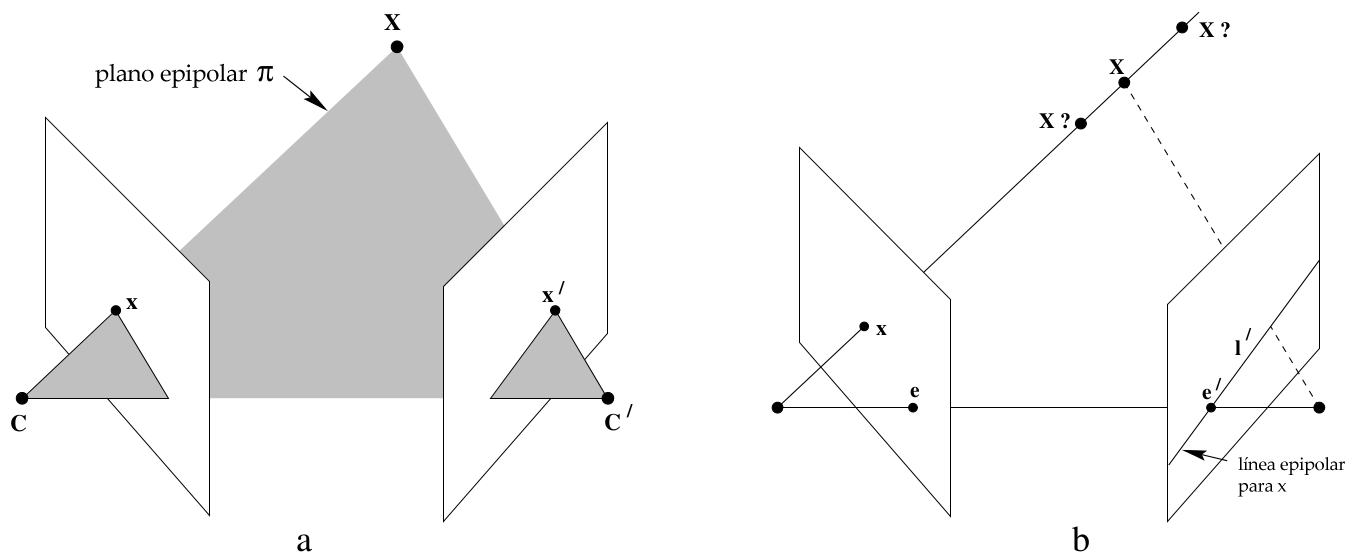
\includegraphics[width=1.0\textwidth]{images/pointcorrespgeom.png}
\caption[Geometr\'{i}a de correspondencia de puntos]%
{\textbf{(a)} Las dos c\'{a}maras son indicadas por sus centros \textbf{C} y \textbf{C'} y los planos de las im\'{a}genes. Los centros de las c\'{a}maras, el punto tridimensional \textbf{X} y sus im\'{a}genes \textbf{x} y \textbf{x'} se encuentran todos en un plano com\'{u}n \textbf{$\pi$}. \textbf{(b)} Un punto \textbf{x} de una imagen se retroproyecta hacia un rayo en un espacio tridimensional definido por el primer centro de la c\'{a}mara \textbf{C} y por \textbf{x}. Este rayo se representa como la l\'{i}nea \textbf{l'} en la segunda vista. El punto tridimensional \textbf{X}, el cual se proyecta hacia \textbf{x}, \underline{debe} encontrarse en este rayo, de manera que la imagen de \textbf{X} en la segunda vista debe encontrarse en \textbf{l'}. Imagen tomada del libro \textit{Multiple View Geometry} de Richard Hartley y Andrew Zisserman \copyright \cite{Hartley_Zisserman_2003}.}
\label{fig:PointCorrespondenceFGeometry}
\end{figure}


\begin{figure}[H]
\centering
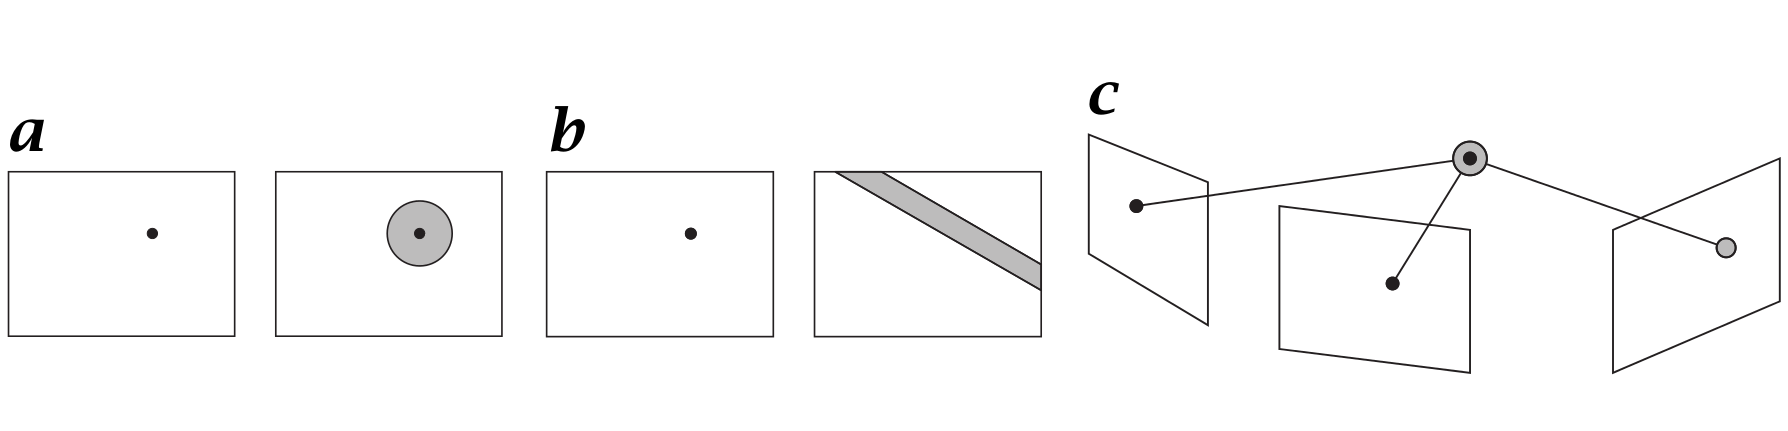
\includegraphics[width=1.0\textwidth]{images/searchregion1.png}
\caption[Restricci\'{o}n del \'{a}rea de b\'{u}squeda de puntos]%
{\textbf{(a)} Imagen con una regi\'{o}n de b\'{u}squeda estimada \textit{a priori}. \textbf{(b)} Regi\'{o}n de b\'{u}squeda estimada utilizando geometr\'{i}a epipolar. \textbf{(c)} Predicci\'{o}n de una regi\'{o}n de b\'{u}squeda despu\'{e}s de una reconstrucci\'{o}n proyectiva del punto (utilizada para refinamiento). Imagen tomada del libro \textit{Handbook of Computer Vision and Applications} de Jahne B. \copyright \cite{Jahne_Haussecker_Geibler_1999}.}
\label{fig:SearchRegion1}
\end{figure}


La matriz fundamental (ll\'{a}mese \textit{\textbf{F}}) encapsula la geometr\'{i}a epipolar la cual es necesaria para la reconstrucci\'{o}n. Se define como una matriz de 3x3 de rango 2 la cual determina la relaci\'{o}n que existe entre puntos clave en pares de im\'{a}genes estereosc\'{o}picas. Si un punto en el espacio tridimensional \textit{X} es proyectado como \textit{x} en la primera vista, y como \textit{x'} en la segunda vista, entonces los puntos de la imagen satisfacen la relaci\'{o}n $x'^TFx = 0$ \cite{Faugeras_1993,Shah_1983,Hartley_Zisserman_2003,Faugeras_Luong_2001}. Esto significa que utilizando geometr\'{i}a epipolar, es posible determinar la matriz fundamental a partir de correspondencia de puntos en pares de im\'{a}genes estereosc\'{o}picas. En \cite{Hartley_Zisserman_2003} se muestran diferentes t\'{e}cnicas para recuperar la matriz fundamental \textit{F} utilizando correspondencia de puntos y a su vez, se prueba que tanto la matriz de rotaci\'{o}n \textit{R} y como la de traslaci\'{o}n \textit{t} pueden ser inferidas a partir de \textit{F}.

Una de las t\'{e}cnicas m\'{a}s sugeridas para encontrar \textit{F} es el algoritmo de correspondencia de 7 puntos descrito en \cite{Faugeras_1993,Hartley_Zisserman_2003}. Pero dado que el mapa de movimiento estimado en la fase anterior permite determinar una cantidad mucho mayor de puntos clave, se opt\'{o} por utilizar la implementaci\'{o}n\footnote{Se utiliz\'{o} la implementaci\'{o}n que viene en la biblioteca de visi\'{o}n artificial conocida como OpenCV.} de un algoritmo m\'{a}s robusto basado en \textit{RANSAC} (del ingl\'{e}s \textit{RANdom SAmple Consensus}).

Publicado por Fischler y Bolles en 1981, se define como un algoritmo iterativo que permite estimar los par\'{a}metros de un modelo matem\'{a}tico a partir de un conjunto de datos observados en los cuales existen valores at\'{i}picos (del ingl\'{e}s \textit{outliers}) \cite{Fischler_Bolles_1981,Chum_2005}. RANSAC es utilizado a menudo en el \'{a}rea de la visi\'{o}n artificial para resolver simult\'{a}neamente el problema de correspondencia de puntos y el de estimaci\'{o}n de la matriz fundamental a partir de un par de im\'{a}genes estereosc\'{o}picas \cite{Forsyth_Ponce_2002,Hartley_Zisserman_2003,Torr_Murray_1997,Chum_2005}.


\begin{figure}[H]
\centering
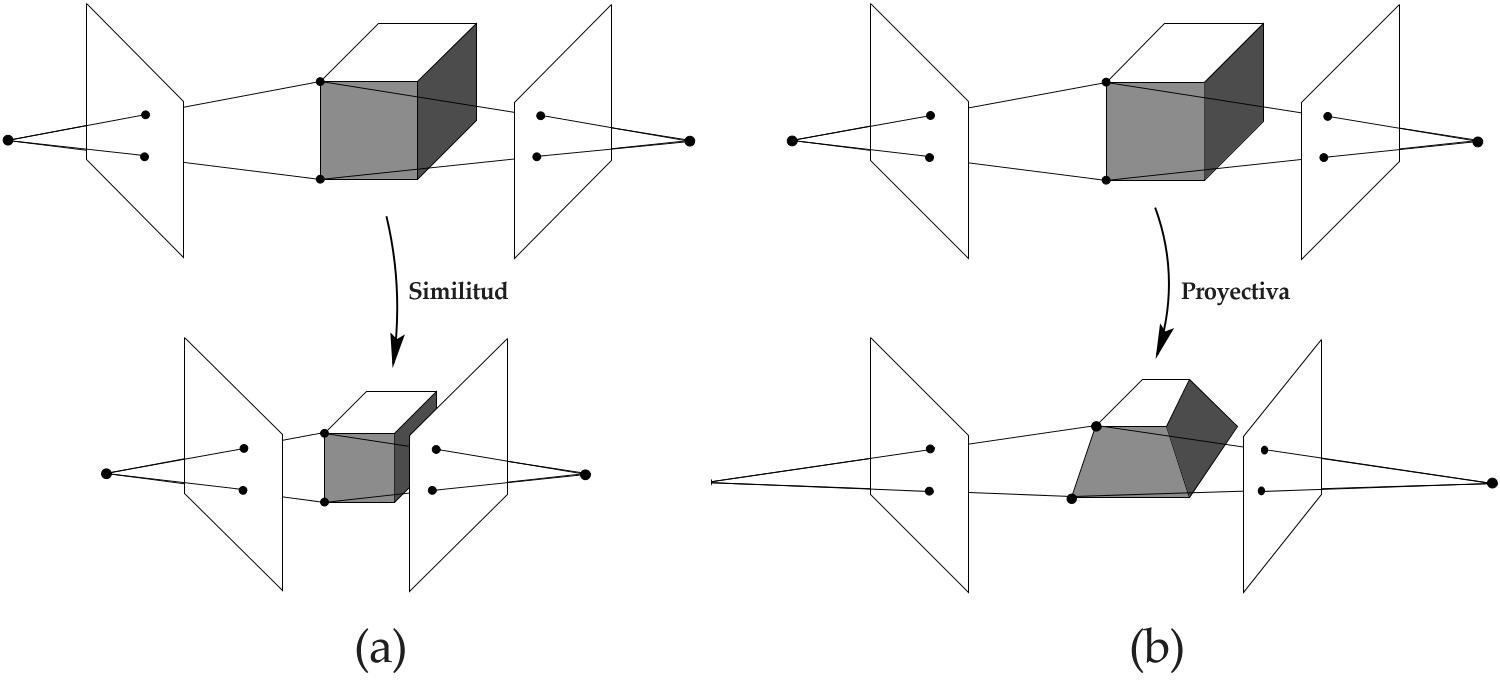
\includegraphics[width=1.0\textwidth]{images/projectiveambiguity1.png}
\caption[Problema de ambigüedad proyectiva]%
{\textbf{(a)} Si las c\'{a}maras est\'{a}n calibradas, cualquier reconstrucci\'{o}n debe respetar el \'{a}ngulo entre los rayos medidos en la imagen. Una transformaci\'{o}n de similitud de la estructura
y posiciones de c\'{a}mara no altera el \'{a}ngulo medido. El \'{a}ngulo entre los rayos y la l\'{i}nea base (epipolos) tampoco son alterados. \textbf{(b)} Si las c\'{a}maras no est\'{a}n calibradas, las reconstrucciones s\'{o}lo deben respetar los puntos de la imagen (la intersecci\'{o}n de los rayos con el plano de la imagen). Una transformaci\'{o}n proyectiva de la estructura y de las posiciones de la c\'{a}mara no altera los puntos medidos, aunque el \'{a}ngulo entre los rayos
s\'{i} es alterado. Los epipolos tampoco son alterados (intersecci\'{o}n con la l\'{i}nea de base). Imagen tomada del libro \textit{Multiple View Geometry} de Richard Hartley y Andrew Zisserman \copyright.}
\label{fig:ReconstructionAmbiguity}
\end{figure}


A pesar de que RANSAC permite encontrar la matriz fundamental, existe el problema de ambigüedad proyectiva que se muestra en la figura ~\ref{fig:ReconstructionAmbiguity}. Esto significa que la matriz obtenida podr\'{i}a no ser la real dado que es posible que haya sido afectada por una transformaci\'{o}n tridimensional proyectiva \cite{Hartley_Zisserman_2003}. Para lidiar con este problema, se necesita encontrar otra matriz conocida como la matriz esencial \textit{\textbf{E}} \cite{Longuet_Higgins_1981}, la cual es una matriz con caracter\'{i}sticas muy similares a la matriz fundamental con la excepci\'{o}n de que s\'{o}lo se utiliza en c\'{a}maras calibradas. Esto permite remover la ambigüedad proyectiva y a su vez, permite realizar una reconstrucci\'{o}n m\'{e}trica, lo cual significa que los puntos tridimensionales est\'{a}n sujetos a una escala verdadera y no a una de transformaci\'{o}n proyectiva \cite{Cyganek_Siebert_2009,Hartley_Zisserman_2003,Szeliski_2010}.

Similar a la matriz fundamental, la matriz esencial \textit{\textbf{E}} tiene una dimensi\'{o}n de 3x3 e impone restricciones entre un punto de una imagen y un punto en la otra imagen de manera que $x'Ex = 0$, donde \textit{x} es un punto en una imagen y \textit{x'} es el punto correspondiente en la otra imagen. Para el c\'{a}lculo de la matriz esencial \textit{E} se utiliz\'{o} la siguiente ecuaci\'{o}n descrita en \cite{Szeliski_2010,Hartley_Zisserman_2003}:


\vspace{5 mm}
\begin{center}
$\mathbf{E = K'^TFK}$
\end{center}
\vspace{5 mm}


Utilizando la ecuaci\'{o}n anterior, es posible determinar la matriz esencial \textit{\textbf{E}} a partir de la matriz de la calibraci\'{o}n de la c\'{a}mara \textit{\textbf{K}} y la matriz fundamental \textit{\textbf{F}}. Una vez obtenida \textit{\textbf{E}}, se necesita extraer el elemento de rotaci\'{o}n \textit{\textbf{R}} y el de traslaci\'{o}n \textit{\textbf{t}} que se encuentran contenidos en ella.

Cabe destacar que la matriz \textit{E} s\'{o}lo brinda una de las dos c\'{a}maras\footnote{Por simplicidad, el t\'{e}rmino c\'{a}mara o matrices de la c\'{a}mara se utiliza indistintamente.} necesarias para la reconstrucci\'{o}n. Para obtener la otra c\'{a}mara se procede a fijar (no rotaci\'{o}n ni traslaci\'{o}n) una de las c\'{a}maras (ll\'{a}mese \textit{\textbf{P}}) y luego se calcula el elemento de rotaci\'{o}n \textit{R} y traslaci\'{o}n \textit{t} de la otra c\'{a}mara (ll\'{a}mese \textit{\textbf{P'}}) con respecto a \'{e}sta. Esto significa que cualquier punto tridimensional que se obtenga a partir de este par de c\'{a}maras tendr\'{a} su primera c\'{a}mara ubicada en la coordenada origen (0,0,0) y su segunda c\'{a}mara estar\'{a} ubicada en \textit{t} \cite{hartley1997triangulation,Hartley_Zisserman_2003}.

Se utiliz\'{o} la t\'{e}cnica de decomposici\'{o}n en valores singulares (del ingl\'{e}s \textit{singular value decomposition}) \cite{Wang_Tsui_2000} en conjunto con el c\'{a}lculo de las cuatro soluciones para reconstrucci\'{o}n calibrada detallado en \cite{Hartley_Zisserman_2003} para extraer los elementos de rotaci\'{o}n y traslaci\'{o}n de la segunda c\'{a}mara.


\begin{figure}[H]
\centering
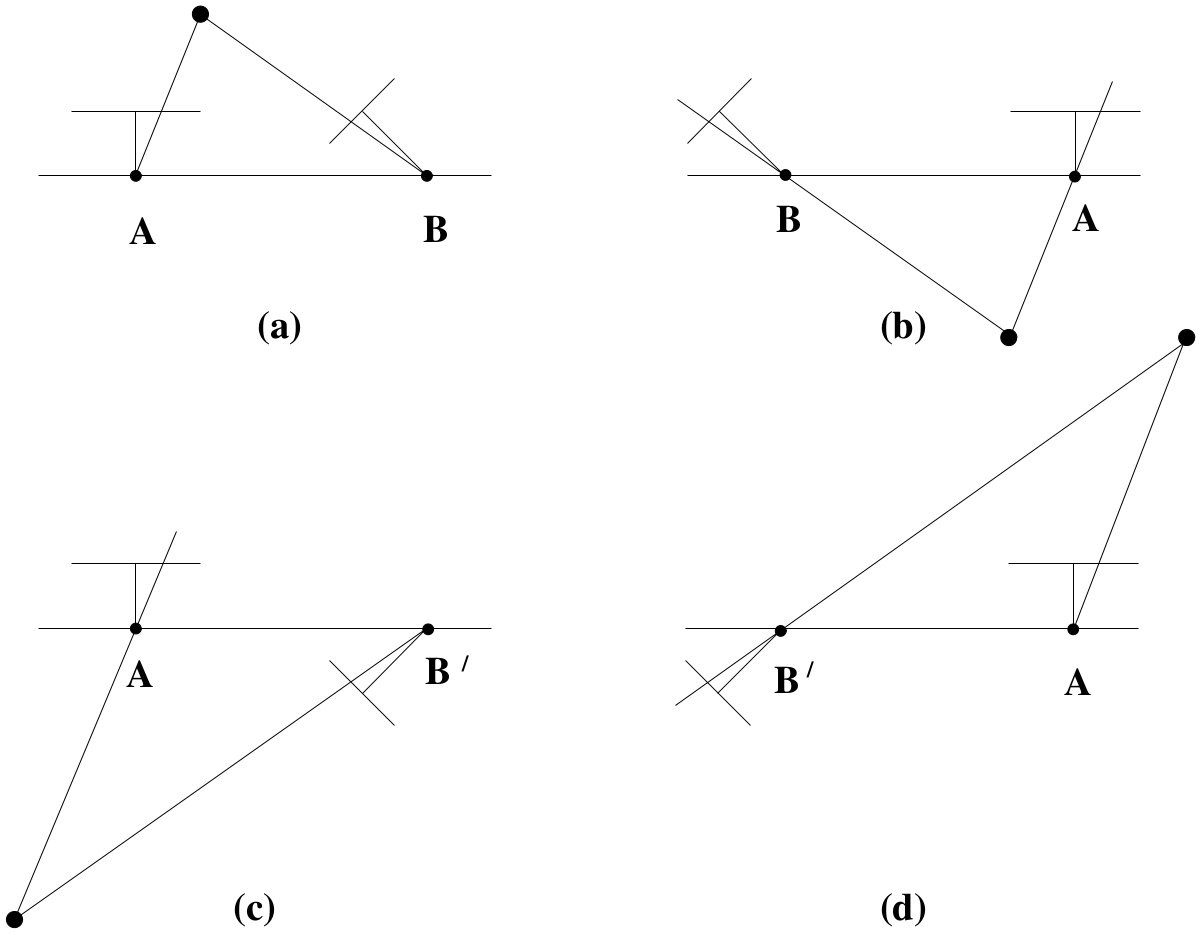
\includegraphics[width=1.0\textwidth]{images/foursolution1.png}
\caption[Cuatro posibles soluciones para reconstrucci\'{o}n calibrada usando \textit{E}]%
{Entre los lados izquierdo y derecho existe una inversi\'{o}n de la l\'{i}nea base. Entre las filas de arriba y abajo la c\'{a}mara \textit{B} rota $180^\circ$ sobre la l\'{i}nea base. N\'{o}tese que s\'{o}lo \textbf{(a)} es la reconstrucci\'{o}n del punto cuando \'{e}ste se encuentra frente a ambas c\'{a}maras. Imagen tomada del libro \textit{Multiple View Geometry} de Richard Hartley y Andrew Zisserman \copyright.}
\label{fig:FourSolutions1}
\end{figure}

Las cuatro posibles soluciones se ilustran en la figura ~\ref{fig:FourSolutions1}, donde se muestra que un punto reconstruido \textit{X} estar\'{a} frente a ambas c\'{a}maras solamente en una de cuatro las soluciones. De \'{e}sta forma basta probar con un solo punto para determinar si est\'{a} frente a ambas c\'{a}maras y as\'{i} decidir entre las cuatro diferentes soluciones para la matriz de la c\'{a}mara \textit{P'} \cite{Hartley_Zisserman_2003}.

El siguiente paso en la t\'{e}cnica es utilizar las matrices estimadas ($P$ y $P'$) de la c\'{a}mara para calcular la distancia de los puntos del objeto a reconstruir. A esta fase se le conoce como estimaci\'{o}n de la profundidad.

%@TODO resumen del capitulo
\chapter{Estimaci\'{o}n de la profundidad}
\label{chap:profundidad}
\epigraph{The most powerful source of human depth perception is stereopsis, the response created in our visual systems by comparing the views we get from our two eyes.}{Barry Hochfelder}

En este cap\'{i}tulo se describe el proceso utilizado para la recuperaci\'{o}n de la profundidad de los puntos del objeto. El m\'{e}todo utilizado popularmente es triangulaci\'{o}n. Para la t\'{e}cnica se utiliz\'{o} uno de los algoritmos propuestos por \cite{hartley1997triangulation}. Cabe destacar la importancia en la selecci\'{o}n del algoritmo de triangulaci\'{o}n dado su papel en la calidad de la representaci\'{o}n tridimensional que se obtenga.

\section{Triangulaci\'{o}n}
Recobrar la dimensi\'{o}n perdida (profundidad) de un punto que aparece en un par de im\'{a}genes bidimensionales estereosc\'{o}picas es uno de los problemas m\'{a}s desafiantes en el \'{a}rea de la visi\'{o}n artificial. Para estimar la estructura tridimensional del objeto se deben utilizar las matrices de la c\'{a}mara \textit{P} y \textit{P'} en conjunto con un algoritmo robusto de triangulaci\'{o}n. %Se asume que solamente existen errores en la medici\'{o}n de las coordenadas de la imagen y no en las matrices \textit{P}, \textit{P'}.

De acuerdo con \cite{hartley1997triangulation}, triangulaci\'{o}n se define como el problema de encontrar la posici\'{o}n de un punto en el espacio tridimensional dada su posici\'{o}n en dos im\'{a}genes tomadas con c\'{a}maras de las cuales son conocidos sus valores de calibraci\'{o}n y su posici\'{o}n. Este proceso, requiere la intersecci\'{o}n de dos rayos conocidos en el espacio. En la figura ~\ref{fig:IdealTriangulation} se muestra el caso ideal del proceso de triangulaci\'{o}n.

\begin{figure}[H]
\centering
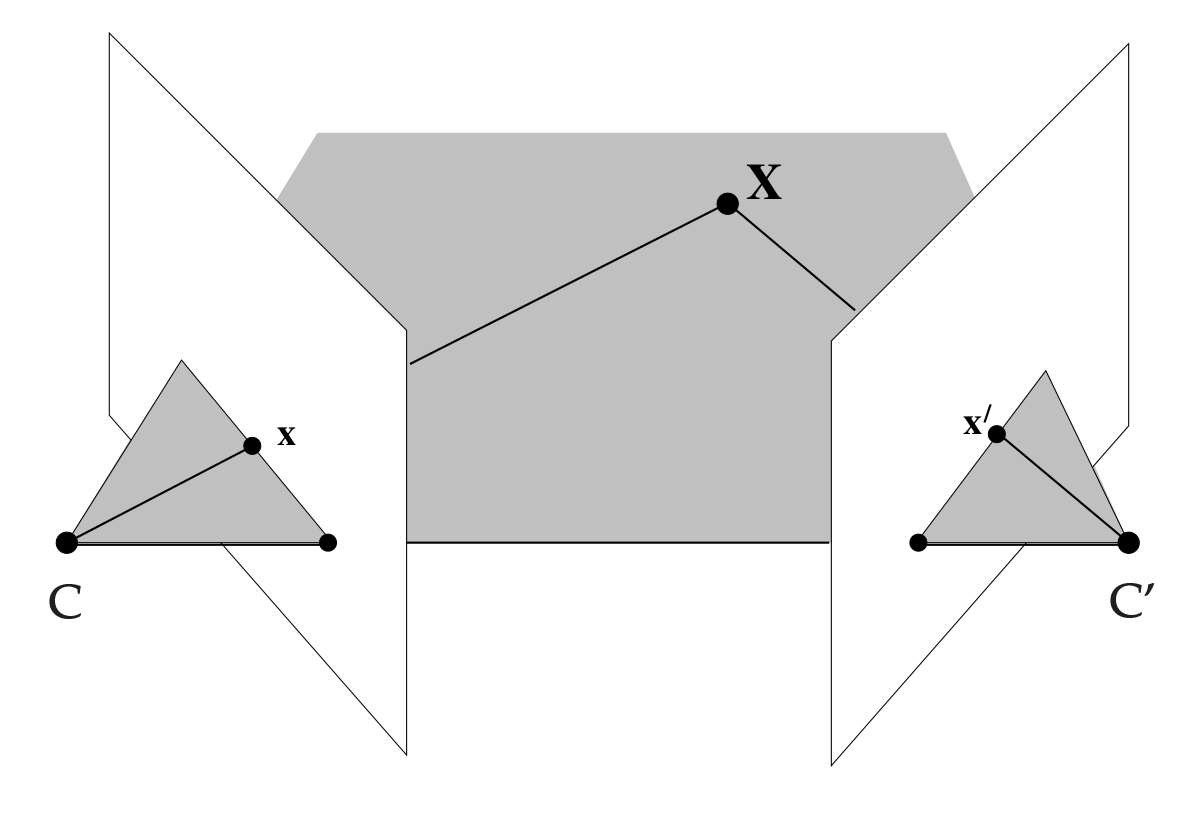
\includegraphics[width=0.8\textwidth]{images/idealtriangulation.png}
\caption[Caso ideal del proceso de triangulaci\'{o}n]%
{Caso ideal de geometr\'{i}a epipolar. Un punto tridimensional \textit{\textbf{X}} es proyectado en dos c\'{a}maras por medio de las l\'{i}neas las cuales se intersecan con el punto focal de cada c\'{a}mara \textbf{\textit{$C$}} y \textbf{\textit{$C'$}}. Los puntos de la imagen resultante son \textbf{\textit{$x$}} y \textbf{\textit{$x'$}}. Las l\'{i}neas se intersecan en \textit{\textbf{X}}. Imagen tomada del libro \textit{Multiple View Geometry} de Richard Hartley y Andrew Zisserman \copyright.}
\label{fig:IdealTriangulation}
\end{figure}

En ausencia de ruido, el problema es trivial. Dado que cada punto en una imagen corresponde a una l\'{i}nea en el espacio tridimensional, todos los puntos de la l\'{i}nea son proyectados en el punto de la imagen. Si es posible encontrar un par de puntos que corresponden en dos o m\'{a}s im\'{a}genes, debe ser el caso en el cual son la proyecci\'{o}n de un punto tridimensional com\'{u}n \textbf{\textit{x}}. El grupo de l\'{i}neas generadas por los puntos de la imagen deben intersecar en \textit{x} y la f\'{o}rmula algebraica para determinar las coordenadas de \textit{x} puede ser calculada utilizando alguno de los muchos m\'{e}todos existentes \cite{hartley1997triangulation,Hartley_Zisserman_2003,Faugeras_1993}.

En la pr\'{a}ctica nada de esto funciona debido la enorme cantidad de ruido (ruido geom\'{e}trico, distorsi\'{o}n del lente, error en los pareos, entre otros) que existe. Esto causa que los dos rayos generalmente no se intersecten por lo que es necesario encontrar el \textit{mejor} punto de la intersecci\'{o}n. En la figura ~\ref{fig:RealTriangulation} se muestra el caso real del proceso de triangulaci\'{o}n.


\begin{figure}[H]
\centering
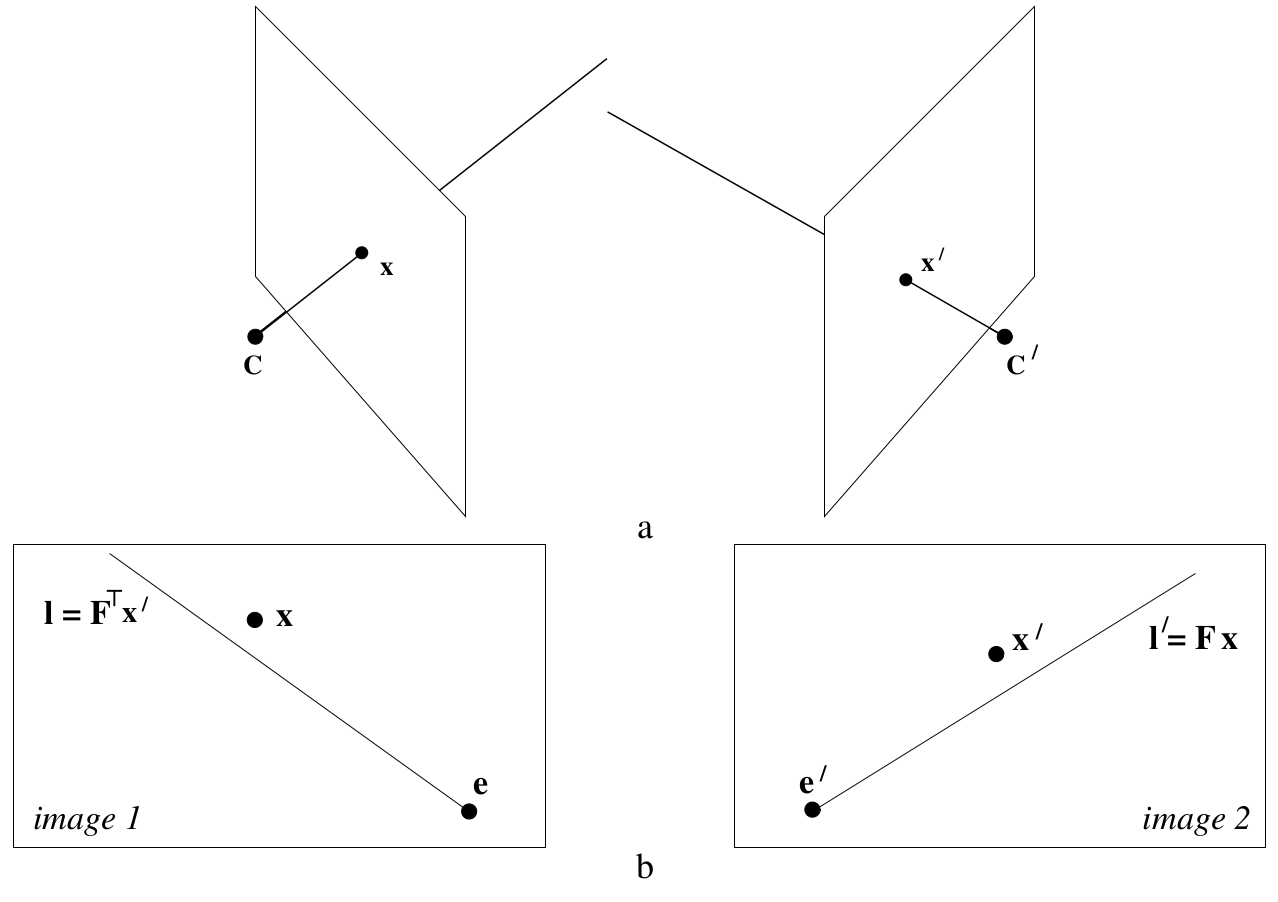
\includegraphics[width=1.0\textwidth]{images/realtriangulation.png}
\caption[Caso real del proceso de triangulaci\'{o}n]%
{En la pr\'{a}ctica, los puntos \textbf{\textit{$x$}} y \textbf{\textit{$x'$}} de la imagen no pueden ser calculados con precisi\'{o}n arbitraria. \textbf{(a)} Los rayos retroproyectados a partir de medidas imperfectas en los puntos \textit{x} y \textit{x'} son generalmente oblicuos en el espacio tridimensional. \textit{(b)} La geometr\'{i}a epipolar para \textbf{\textit{$x$}} y \textbf{\textit{$x'$}}. Los puntos medidos no satisfacen la restricci\'{o}n epipolar. La l\'{i}nea epipolar $l' = Fx$ es la imagen del rayo a trav\'{e}s de \textit{x} y $l = F^Tx'$ es la imagen del rayo a trav\'{e}s de \textit{x'}. Dado que los rayos no se intersecan, \textit{x'} no se encuentra en \textit{l'} y \textit{x} no se encuentra en \textit{l}. Imagen tomada del libro \textit{Multiple View Geometry} de Richard Hartley y Andrew Zisserman \copyright.}
\label{fig:RealTriangulation}
\end{figure}


La importancia en la selecci\'{o}n de un buen algoritmo de triangulaci\'{o}n se muestra claramente en \cite{Beardsley_Zisserman_Murray_1997,beardsley_etal_eccv1994}. En \cite{hartley1997triangulation} se presenta una detallada comparaci\'{o}n entre diferentes algoritmos de triangulaci\'{o}n. En su apartado de resultados se muestra la duraci\'{o}n relativa en tiempo de cada algoritmo as\'{i} como las condiciones bajo las cuales es recomendable utilizar uno en favor del otro. 

Para la t\'{e}cnica de reconstrucci\'{o}n propuesta, se opt\'{o} por utilizar el algoritmo iterativo de m\'{i}nimos cuadrados (del ingl\'{e}s \textit{iterative linear least squares}) descrito en \cite{hartley1997triangulation,Hartley_Zisserman_2003}, dado que seg\'{u}n los resultados de rendimiento mostrados en el art\'{i}culo, es uno de los m\'{a}s r\'{a}pidos (3 veces m\'{a}s que el algoritmo polinomial recomendado por los autores del art\'{i}culo) y desempe\~na bien en reconstrucci\'{o}n tridimensional.

El siguiente paso en la t\'{e}cnica es utilizar las matrices de la c\'{a}mara, el algoritmo de triangulaci\'{o}n y los pareos de puntos clave de la primera fase, para determinar la posici\'{o}n en el espacio tridimensional de cada uno de ellos y as\'{i} reconstruir el objeto en cuesti\'{o}n.

%@TODO resumen del capitulo

%Su \'{u}nico problema es que en ciertos casos no converge y por lo tanto se debe contar con un algoritmo de respaldo.

%@TODO poner screenshots de ejemplos de triangulaci\'{o}n ???
%@TODO es necesario explicar el algoritmo de minimos cuadrados o no???

%\section{Algoritmo iterativo de m\'{i}nimos cuadrados}

%Once we have two camera matrices, P and P', we can recover the 3D structure of the scene. This can be seen simply if we think about it using ray intersection. We have two points in space of the camera centers (one in 0,0,0 and one in t), and we have the location in space of a point both on the image plane of image 1 and on the image plane of image 2. If we simply shoot a ray from from one camera center through the respective point and another ray from the other camera - the intersection of the two rays must be the real location of the object in space.
%In real life, none of that works. The rays usually will not intersect (so H&Z refer to the mid-point algorithm, which they dismiss as a bad choice), and ray intersection in general is inferior to other triangulation methods.
%H&Z go on to describe their "optimal" triangulation method, which optimizes the solution based on the error from reprojection of the points back to the image plane.
%I have implemented the linear triangulation methods they present, and wrote a post about it not long ago: Here.
%I also added the Iterative Least Squares method that Hartley presented in his article "Triangulation", which is said to perform very good and very fast.


\chapter{Reconstrucci\'{o}n tridimensional}
\label{chap:reconstruccion}
\epigraph{Going from the written, flat word to the three-dimensional object, that was one of the more enriching things that I've done.}{James Sanborn}

%@TODO que no se hizo/alcances/hipotesis
En este cap\'{i}tulo se describe c\'{o}mo utilizar la informaci\'{o}n obtenida hasta el momento para reconstruir tridimensionalmente el objeto. Las matrices de la c\'{a}mara (fundamental y esencial) permiten, en conjunto con el algoritmo de triangulaci\'{o}n, estimar la profundidad en el espacio tridimensional de cada uno de los pareos de puntos clave obtenidos a partir del par de im\'{a}genes estereosc\'{o}picas.

\section{Reconstrucci\'{o}n base con dos vistas}
De acuerdo con \cite{Hartley_Zisserman_2003}, si se tiene un conjunto de correspondencias de puntos $x_i \leftrightarrow 
 x'_i$ provenientes de un grupo de puntos tridimensionales $X_i$ no conocidos, de igual forma, la posici\'{o}n, orientaci\'{o}n y los valores de calibraci\'{o}n de la c\'{a}mara tampoco son conocidos, la tarea de reconstrucci\'{o}n es encontrar las matrices \textit{$P$} y \textit{$P'$} as\'{i} como los puntos tridimensionales \textit{$X_i$} de manera que:

\vspace{5 mm}
\begin{center}
\textbf{\textit{$x_i$}} = \textbf{\textit{$PX_i$}} 
\textbf{\textit{$x'_i$}} = \textbf{\textit{$P'X_i$}}
para todo \textit{$i$}
\end{center}
\vspace{5 mm}

Con una cantidad suficiente de correspondencias de puntos clave es posible calcular la matriz fundamental y a partir de ah\'{i}, realizar una reconstrucci\'{o}n proyectiva ambigua \cite{hartley1997triangulation,Hartley_Zisserman_2003,Faugeras_1993}. En la figura ~\ref{fig:ProjectiveReconstruction} se muestra un ejemplo de reconstrucci\'{o}n proyectiva.


\begin{figure}[H]
\centering
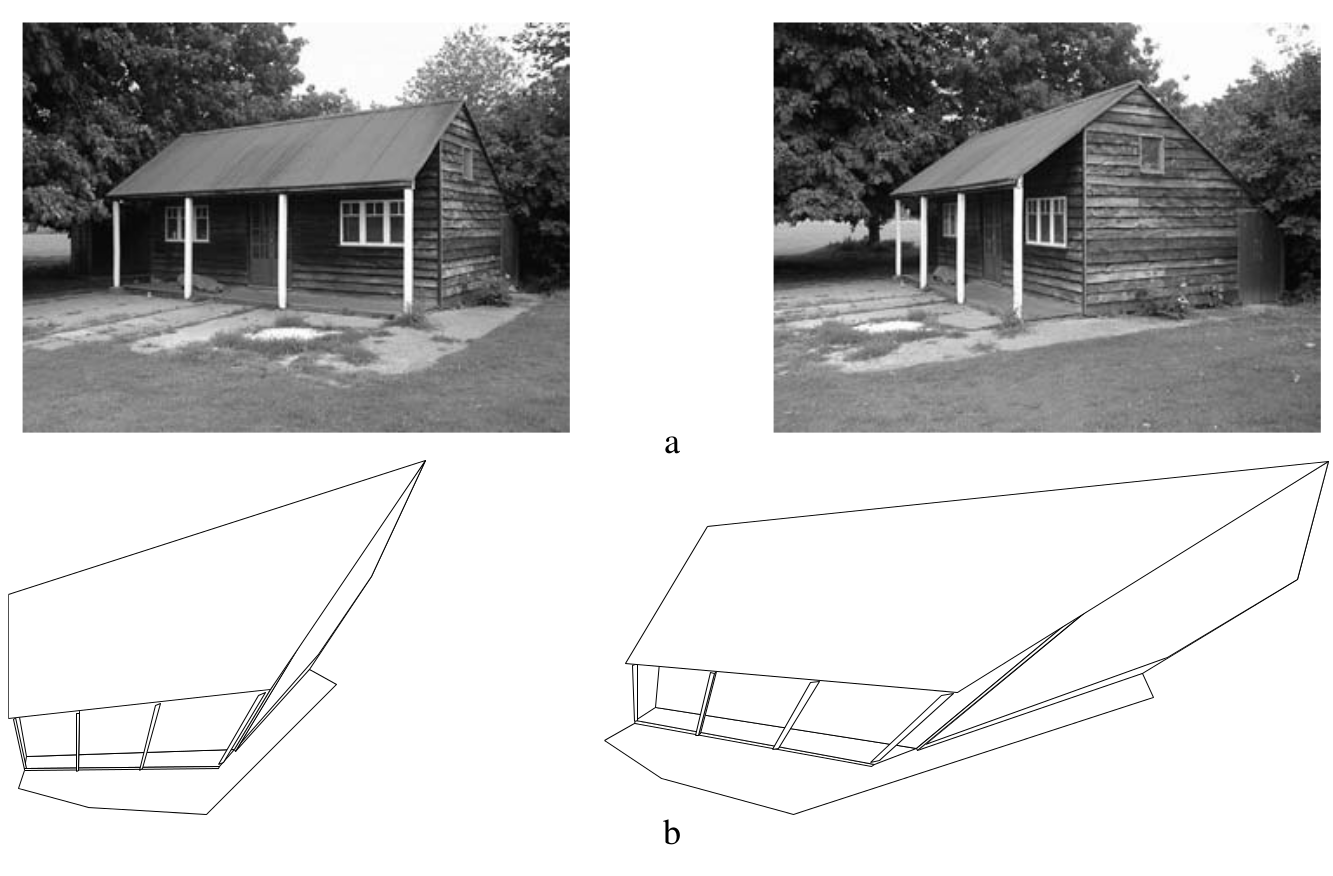
\includegraphics[width=1.0\textwidth]{images/projectivereconstruction.png}
\caption[Reconstrucci\'{o}n proyectiva]%
{\textbf{(a)} Par de im\'{a}genes originales. \textbf{(b)} Dos vistas de una reconstrucci\'{o}n proyectiva de la escena. La reconstrucci\'{o}n no requiere informaci\'{o}n acerca de las matrices de la c\'{a}mara o de la geometr\'{i}a de la escena. La matriz fundamental \textit{F} se calcula a partir de correspondencia de puntos entre el par de im\'{a}genes. Las matrices de la c\'{a}mara se obtienen a partir de \textit{F} y finalmente, los puntos tridimensionales son calculados por medio de triangulaci\'{o}n a partir de las correspondencias. Imagen tomada del libro \textit{Multiple View Geometry} de Richard Hartley y Andrew Zisserman \copyright.}
\label{fig:ProjectiveReconstruction}
\end{figure}


Sin embargo, para la t\'{e}cnica propuesta se busca una reconstrucci\'{o}n m\'{e}trica por lo que para el proceso de estimaci\'{o}n de la profundidad es necesario utilizar la matriz esencial \textit{E} en lugar de la matriz fundamental \textit{F}. En la figura ~\ref{fig:MetricReconstruction} se muestra un ejemplo de reconstrucci\'{o}n m\'{e}trica.


\begin{figure}[H]
\centering
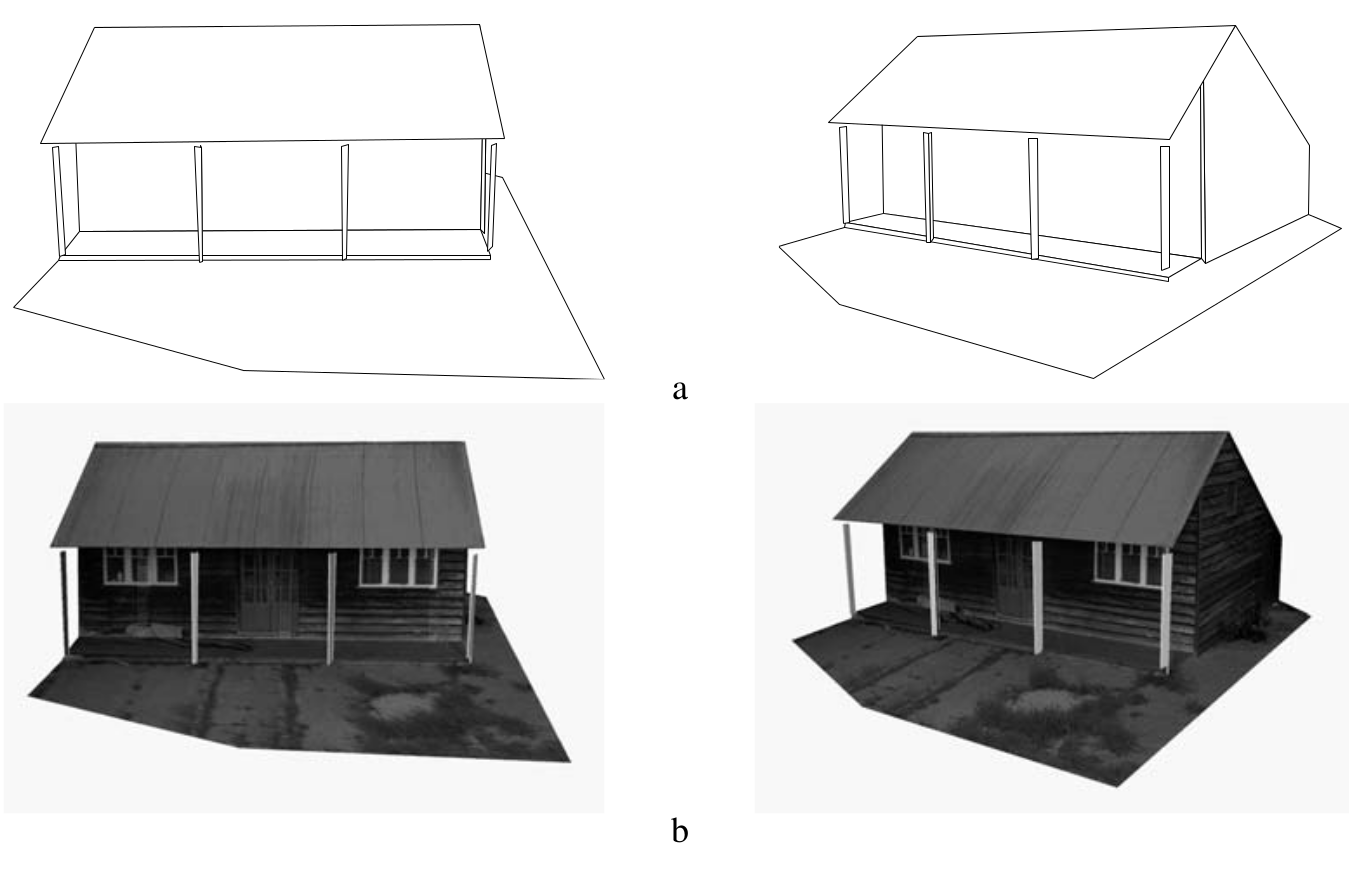
\includegraphics[width=1.0\textwidth]{images/metricreconstruction.png}
\caption[Reconstrucci\'{o}n m\'{e}trica]%
{\textbf{(a)} Dos vistas de la reconstrucci\'{o}n m\'{e}trica. L\'{i}neas que son perpendiculares en la escena son perpendiculares en la reconstrucci\'{o}n y tambi\'{e}n la relaci\'{o}n de aspecto de los lados de la casa es ver\'{i}dico. \textbf{(b)} Dos vistas del modelo reconstruido con textura. Imagen tomada del libro \textit{Multiple View Geometry} de Richard Hartley y Andrew Zisserman \copyright.}
\label{fig:MetricReconstruction}
\end{figure}


Para encontrar la posición de un punto bidimensional en el espacio tridimensional, hay que determinar la posici\'{o}n/orientaci\'{o}n de la c\'{a}mara cuando tom\'{o} la primera imagen (c\'{a}mara P) que contiene a ese punto, luego determinar la posici\'{o}n/orientaci\'{o}n de la c\'{a}mara cuando tom\'{o} la segunda imagen (c\'{a}mara P') de ese mismo punto y finalmente, utilizar el m\'{e}todo lineal de triangulaci\'{o}n seleccionado en la fase anterior. Esto se logra por medio de las ecuaciones $x = PX$ y $x' = P'X$, donde \textit{x} y \textit{x'} son el pareo de puntos bidimensionales y \textit{X} es la posici\'{o}n tridimensional real del punto presentado en ambas c\'{a}maras.

Es posible reescribir las ecuaciones como un sistema lineal que puede resolverse para determinar \textit{X}, lo cual es el objetivo buscado. Ambas ecuaciones se combinan de la forma $AX = 0$, la cual es una ecuaci\'{o}n lineal en \textit{X}. El siguiente planteamiento del sistema de ecuaciones lineales utilizado para la t\'{e}cnica de reconstrucci\'{o}n fue tomado directamente de \cite{Hartley_Zisserman_2003}. Primero, el factor de escala homog\'{e}neo es eliminado con un producto cruzado para obtener tres ecuaciones por cada punto de la imagen, de los cuales dos son linealmente independientes. Por ejemplo, para la primera imagen, $x \times (PX) = 0$ lo cual da:


\vspace{5 mm}
\begin{center}
$x(p^{3T}X) - (p^{1T}X) = 0$ \\
$y(p^{3T}X) - (p^{2T}X) = 0$ \\
$x(p^{2T}X) - y(p^{1T}X) = 0$
\end{center}
\vspace{5 mm}


donde $p^{iT}$ son las filas de la matriz $P$. Estas ecuaciones son lineales en los componentes de \textbf{X}. Una ecuaci\'{o}n de la forma $AX = 0$ puede ser entonces creada con:

\vspace{5 mm}
\begin{center}
$\textbf{\textit{A}} =
\left[ {
\begin{array}{*{20}c}
   xp^{3T} - p^{1T} \\
   yp^{3T} - p^{2T} \\
   x'p'^{3T} - p'^{1T} \\
   y'p'^{3T} - p'^{2T} \\
\end{array} 
} \right]$
\end{center}
\vspace{5 mm}

donde dos ecuaciones han sido incluidas para cada imagen, dando un total de cuatro ecuaciones con cuatro inc\'{o}gnitas homog\'{e}neas. \'{E}ste es un conjunto de ecuaciones redundantes, dado que la soluci\'{o}n es determinada a escala. La descripci\'{o}n completa de la soluci\'{o}n puede encontrarse en \cite{Hartley_Zisserman_2003}. Con la soluci\'{o}n del sistema de ecuaciones anterior es posible obtener una aproximaci\'{o}n de los puntos tridimensionales a partir de dos puntos bidimensionales. 

El proceso final para completar la estructura tridimensional del objeto es iterar sobre cada par de puntos obtenidos, realizar la triangulaci\'{o}n y almacenar el punto tridimensional en una lista para su posterior visualizaci\'{o}n. A continuaci\'{o}n, se muestran diferentes resultados obtenidos con la t\'{e}cnica r\'{a}pida de reconstrucci\'{o}n propuesta.


\begin{figure}[H]
\centering
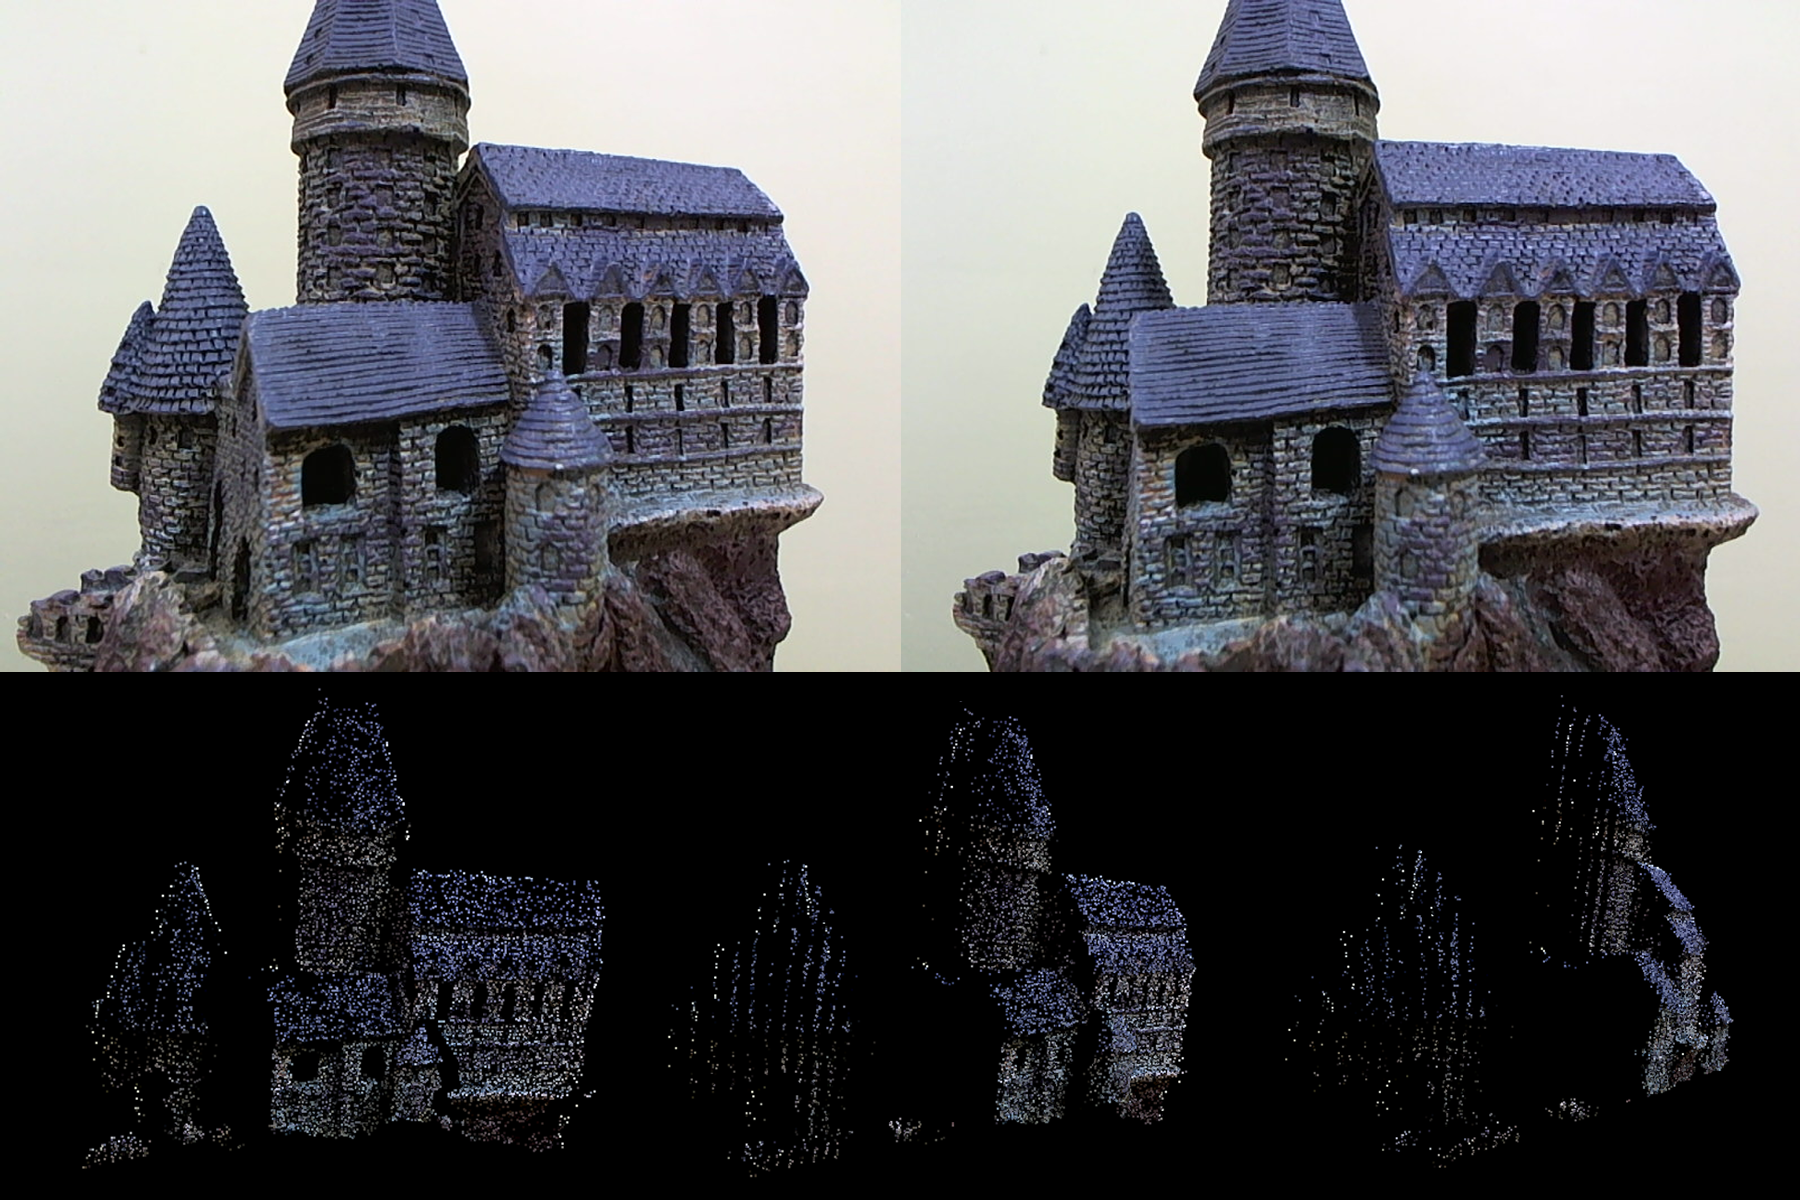
\includegraphics[width=1.0\textwidth]{images/reconstruction1.png}
\caption[Reconstrucci\'{o}n de un costado del castillo]%
{Reconstrucci\'{o}n tridimensional de un costado del casillo utilizando un par de im\'{a}genes estereosc\'{o}picas. N\'{o}tese la densidad de la reconstrucci\'{o}n as\'{i} como la precisi\'{o}n entre las diferentes profundidades del techo y de las torres. Im\'{a}genes generadas con la t\'{e}cnica de reconstrucción propuesta.}
\label{fig:Reconstruction1}
\end{figure}

En la figura ~\ref{fig:Reconstruction1} se muestra la reconstrucci\'{o}n de un costado del castillo a partir de un par de im\'{a}genes estereosc\'{o}picas utilizando la t\'{e}cnica propuesta. N\'{o}tese la densidad de la reconstrucci\'{o}n as\'{i} como la precisi\'{o}n entre las diferentes profundidades del techo y de las torres.


\begin{figure}[H]
\centering
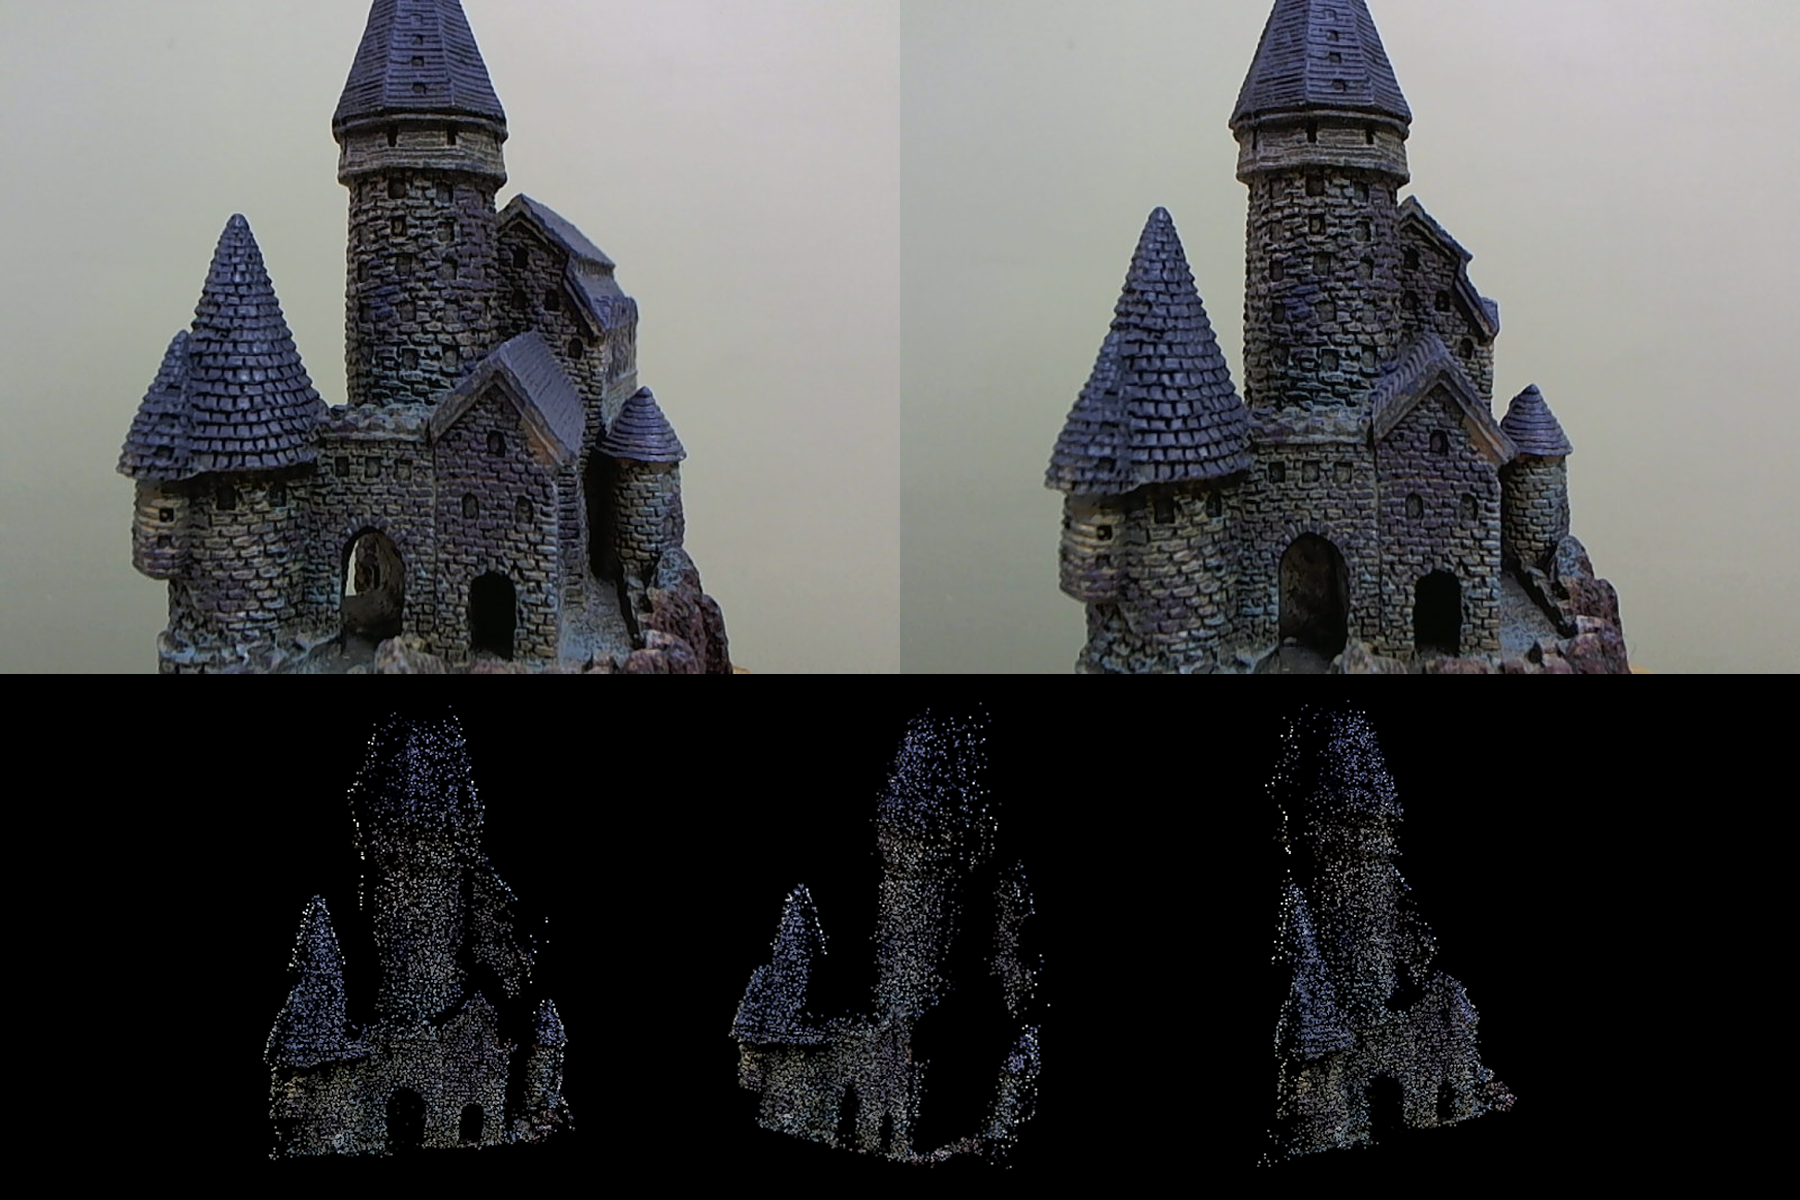
\includegraphics[width=1.0\textwidth]{images/reconstruction2.png}
\caption[Reconstrucci\'{o}n de la fachada del castillo]%
{Reconstrucci\'{o}n tridimensional de la fachada del casillo utilizando un par de im\'{a}genes estereosc\'{o}picas. Nuevamente, n\'{o}tese la precisi\'{o}n de la profundidad entre una torre y la otra. Im\'{a}genes generadas con la t\'{e}cnica de reconstrucción propuesta.}
\label{fig:Reconstruction2}
\end{figure}


En la figura ~\ref{fig:Reconstruction2} se muestra la reconstrucci\'{o}n de la fachada del castillo a partir de un par de im\'{a}genes estereosc\'{o}picas. Nuevamente, n\'{o}tese la precisi\'{o}n de la profundidad reconstruida entre una torre y la otra.


\begin{figure}[H]
\centering
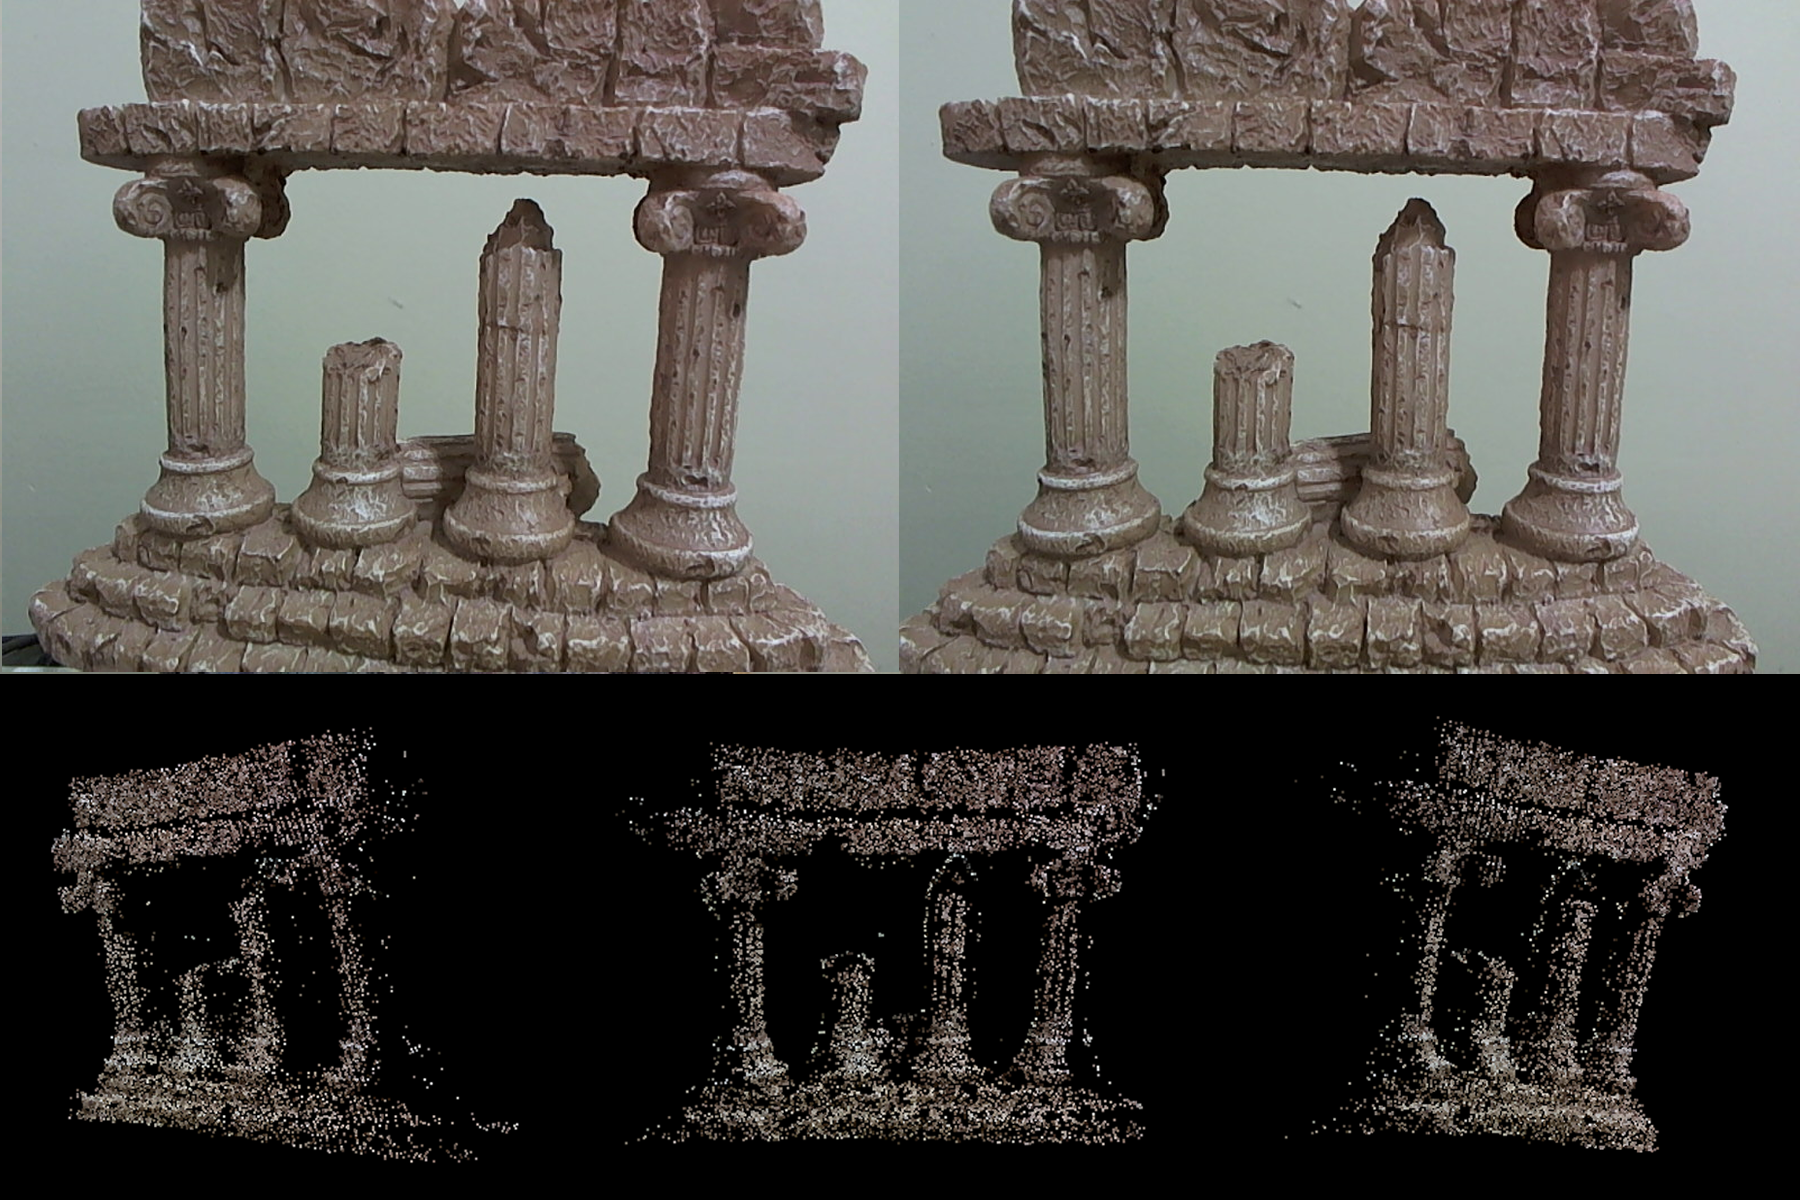
\includegraphics[width=0.9\textwidth]{images/reconstruction3.png}
\caption[Reconstrucci\'{o}n de las columnas Griegas]%
{Reconstrucci\'{o}n tridimensional de las columnas Griegas utilizando un par de im\'{a}genes estereosc\'{o}picas. Por su particular forma, la reconstrucci\'{o}n de este objeto es m\'{a}s compleja que el castillo pero de igual manera se logr\'{o} obtener resultados satisfactorios. Im\'{a}genes generadas con la t\'{e}cnica de reconstrucción propuesta.}
\label{fig:Reconstruction3}
\end{figure}


Finalmente, en la figura ~\ref{fig:Reconstruction3} se muestra la reconstrucci\'{o}n de unas columnas Griegas. A pesar de su particular forma y de la diferencia estructural con respecto al castillo, se logr\'{o} obtener resultados satisfactorios. Cabe destacar que en todos los casos presentados el proceso completo de reconstrucci\'{o}n tom\'{o} no m\'{a}s que unos cuantos segundos.


\section{Reconstrucci\'{o}n con m\'{a}s de dos vistas}
Es posible obtener una reconstrucci\'{o}n a\'{u}n m\'{a}s densa utilizando vistas adicionales del objeto. Para lograr esto se implement\'{o} un m\'{e}todo simple basado en una variante lineal del problema de \textit{Perspective-n-Point} o \textit{PnP} que permite la recuperaci\'{o}n de informaci\'{o}n tridimensional adicional a partir de nuevas vistas del objeto. A la variante se le conoce como \textit{Efficient Perspective-n-Point} o \textit{EPnP}\cite{F_Moreno_V_Lepetit}.

El algoritmo de \textit{PnP} pretende resolver el problema de c\'{o}mo determinar la posici\'{o}n y orientaci\'{o}n de la c\'{a}mara dados sus par\'{a}metros intr\'{i}nsecos m\'{a}s un conjunto de \textit{n} correspondencias entre puntos tridimensionales y sus proyecciones bidimensionales \cite{F_Moreno_V_Lepetit}. Esto significa que con \textit{PnP} es posible estimar la posici\'{o}n de subsecuentes c\'{a}maras (vistas) del objeto a reconstruir utilizando la informaci\'{o}n obtenida (matrices y pareos) en las fases anteriores.

Para incorporar nuevas vistas a la reconstrucci\'{o}n, es necesario encontrar la posici\'{o}n de cada nueva c\'{a}mara utilizando como base la estructura inicial obtenida en la triangulaci\'{o}n de la fase anterior. Para esto se procede a buscar mapeos entre los puntos bidimensionales encontrados en la nueva vista y los puntos tridimensionales ya obtenidos. El objetivo del mapeo es obtener una lista de puntos bidimensionales y otra de puntos tridimensionales en la cual el punto bidimensional \textit{i} corresponde al punto tridimensional \textit{i} dado que es un requisito del algoritmo \textit{EPnP}. Finalmente, se utiliza la matriz \textit{K} en conjunto con los mapeos como entrada del algoritmo de \textit{EPnP} para obtener la posici\'{o}n de la c\'{a}mara (\textit{P1}) de esa nueva vista.

Obtenida la matriz \textit{P1} de la nueva c\'{a}mara, se procede a triangular los puntos de la nueva vista como se realiz\'{o} en la etapa anterior. Finalmente, se almacenan los puntos tridimensionales resultantes en la lista global de puntos 3D y se procede a repetir el proceso para las vistas restantes.

En la figura ~\ref{fig:Castle234} se muestra un ejemplo de reconstrucci\'{o}n con 2, 3 y 4 vistas para el castillo. Cuando la reconstrucci\'{o}n se limita a 2 o 3 vistas la t\'{e}cnica propuesta genera resultados muy satisfactorios como se puede observar en la figura.


\begin{figure}[H]
\centering
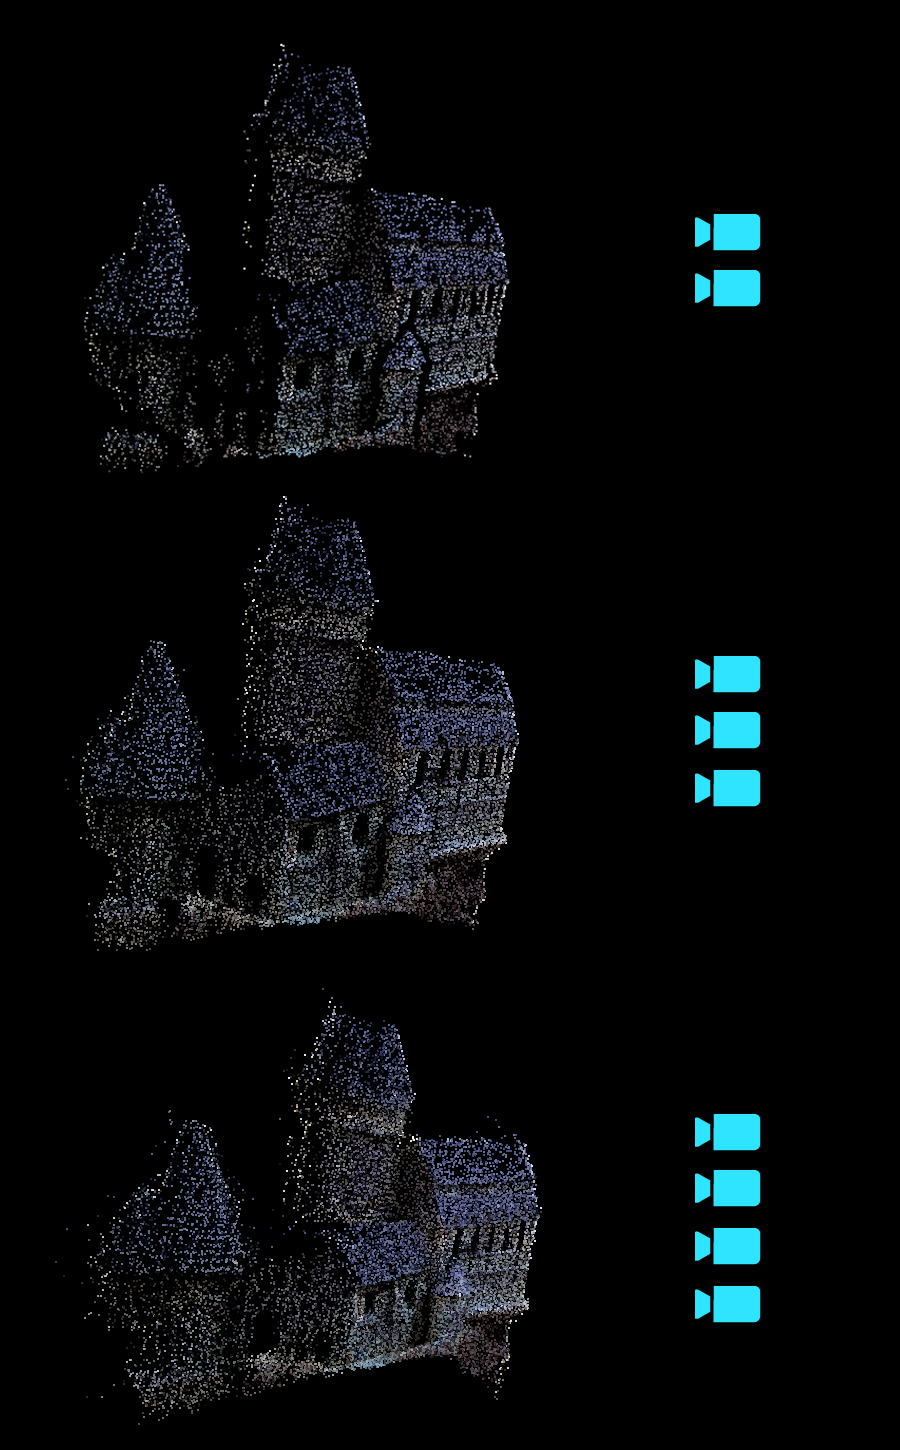
\includegraphics[width=0.8\textwidth]{images/castle234.png}
\caption[Reconstrucci\'{o}n del casillo con 2, 3 y 4 vistas]%
{Reconstrucci\'{o}n tridimensional del castillo con 2, 3 y 4 vistas. La necesidad de una etapa de refinamiento se nota m\'{a}s claramente en la reconstrucci\'{o}n con cuatro vistas. Im\'{a}genes generadas con la t\'{e}cnica de reconstrucción propuesta.}
\label{fig:Castle234}
\end{figure}


Sin embargo, cuando se incrementa a 4 o m\'{a}s vistas los nuevos puntos triangulados no se encuentran completamente alineados con los triangulados previamente. Esto se debe a que cada reconstrucci\'{o}n obtenida a partir del par de im\'{a}genes estereosc\'{o}picas posee su propia escala la cual es totalmente independiente de las escalas de las siguientes reconstrucciones. Una forma de atacar este problema es introducir una etapa de refinamiento y registro al final de cada reconstrucci\'{o}n pero dichas etapas no forman parte de esta tesis.

\begin{figure}[H]
\centering
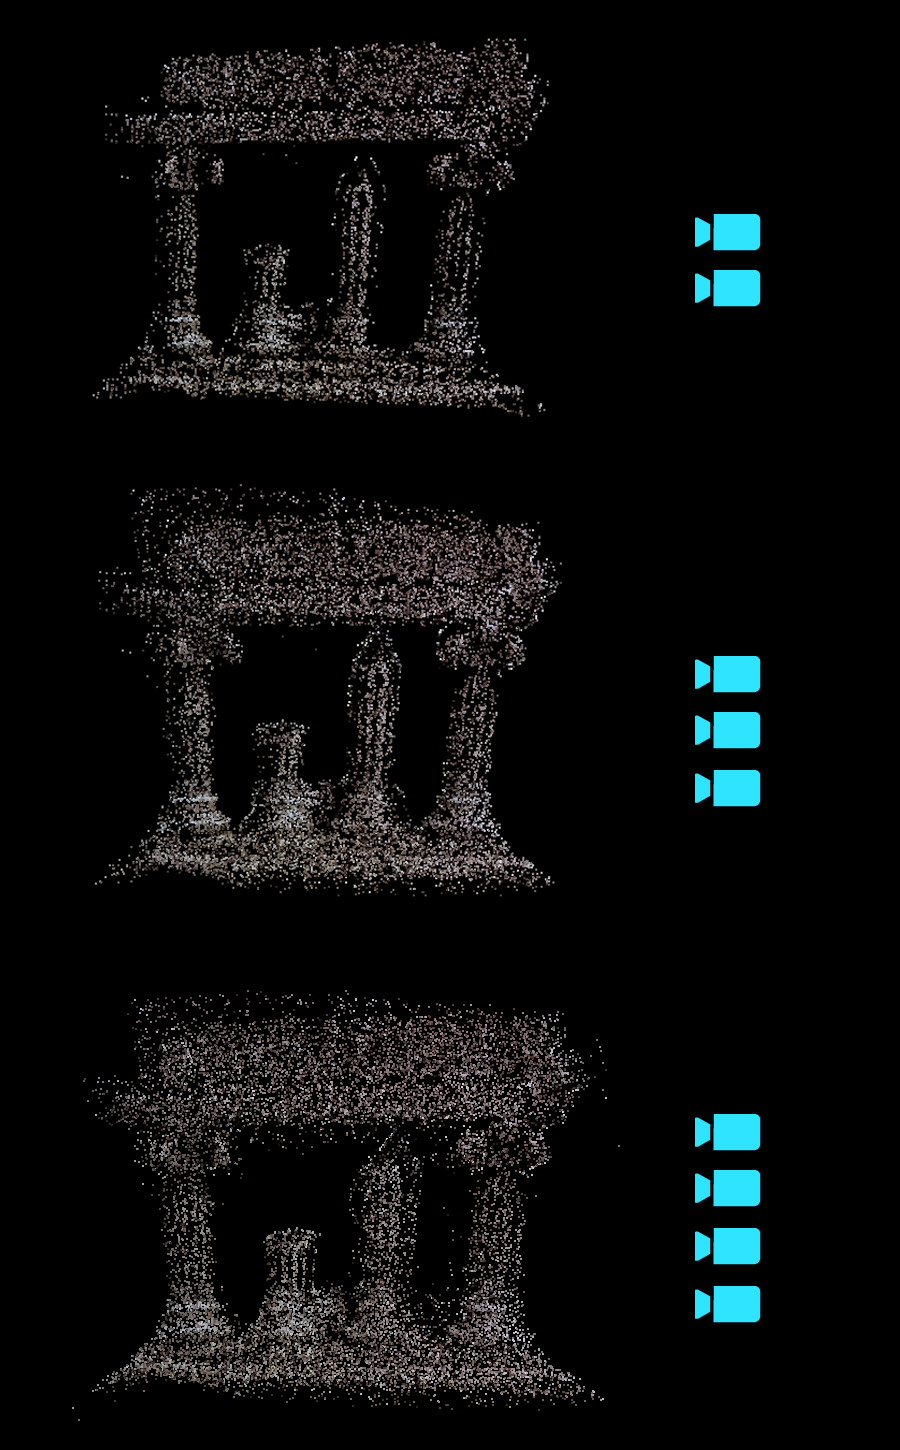
\includegraphics[width=0.8\textwidth]{images/greek234.png}
\caption[Reconstrucci\'{o}n de las columnas Griegas con 2, 3 y 4 vistas]%
{Reconstrucci\'{o}n tridimensional las columnas Griegas con 2, 3 y 4 vistas. Nuevamente, se nota la necesidad de una etapa de refinamiento en este caso a partir de la reconstrucci\'{o}n con tres vistas. Im\'{a}genes generadas con la t\'{e}cnica de reconstrucción propuesta.}
\label{fig:Greek234}
\end{figure}


En la figura ~\ref{fig:Greek234} se muestra otro ejemplo de reconstrucci\'{o}n con 2, 3 y 4 vistas para las columnas Griegas. Nuevamente se puede observar que con 2 vistas la reconstrucci\'{o}n es bastante satisfactoria pero en este caso a partir de la vista 3, la reconstrucci\'{o}n se ve afectada por la falta de las etapas de refinamiento y registro.

Cabe destacar que para lograr la reconstrucci\'{o}n completa de un objeto es necesaria la incorporaci\'{o}n de etapas de refinamiento y registro, sin embargo ambas etapas est\'{a}n fuera de los alcances de esta tesis y se dejar\'{a}n para trabajo futuro.


%@TODO hablar de reconstrucción utilizando multiples vistas, del error de retroproyección y de que bundle adjusment refinaria aun mas la reconstruccion. Hablar de que no se hizo registracion por lo que no hay reconstruccion completa.

%@TODO resumen del capitulo

\chapter{Algoritmo}
\label{chap:algoritmo}
\epigraph{An algorithm must be seen to be believed.}{Donald Knuth}

%En este cap\'{i}tulo se describe el pseudoc\'{o}digo del algoritmo de reconstrucci\'{o}n r\'{a}pida propuesto en esta tesis. Adicionalmente, se brinda su an\'{a}lisis de complejidad y finalmente, las principales diferencias con t\'{e}cnicas similares de reconstrucci\'{o}n.

En este cap\'{i}tulo se describe el pseudoc\'{o}digo del algoritmo de reconstrucci\'{o}n r\'{a}pida propuesto en esta tesis y posteriormente, las principales diferencias con t\'{e}cnicas similares de reconstrucci\'{o}n.

\section{Pseudoc\'{o}digo}
A continuaci\'{o}n se presenta un extracto del m\'{e}todo principal del algoritmo propuesto para la t\'{e}cnica r\'{a}pida de reconstrucci\'{o}n tridimensional. El pseudoc\'{o}digo completo se encuentra en el apartado de ap\'{e}ndices bajo la secci\'{o}n ~\ref{chap:apendice}. Cabe destacar que el experimento fue implementado con C++, Java y OpenCV.
\newpage
\begin{alltt}
\textbf{reconstructor_3d}
  ...
  \textbf{ejecutar}()
    calibrar_camara();
    capturar_vistas();
    pareo_de_puntos();
    eliminar_pareos_erroneos();
    encontrar_triangulacion_base();
    \textbf{para} cada nueva vista \textbf{hacer}
      recuperar_nueva_vista();
    \textbf{fin}
  \textbf{fin}
\textbf{fin}
\end{alltt}

%\section{An\'{a}lisis de complejidad}
%@TODO no se prometió hacerlo, Torres??

\section{Novedad}
Tradicionalmente, se utilizan t\'{e}cnicas de pareo de caracter\'{i}sticas sobresalientes en lugar de t\'{e}cnicas de rastreo denso para reconstrucci\'{o}n tridimensional. Esto se debe a que son consideradas m\'{a}s r\'{a}pidas, m\'{a}s estables y desempe\~nan mejor en im\'{a}genes que poseen una separaci\'{o}n espacial grande \cite{Liu_Cheng_2008,Peng_Chen_Zhou_Liu_2009,Wang_Quan_2008,Ying_Hong-e_Ben-zhi_2010}. Sin embargo, es conocido que el resultado de realizar una reconstrucci\'{o}n basada en pareo de caracter\'{i}sticas sobresalientes generalmente tiende a ser disperso (pocos puntos).

La novedad de la t\'{e}cnica se encuentra en la utilizaci\'{o}n de algoritmos de rastreo denso de pixeles (\textit{Farnebäck}) en conjunto con una t\'{e}cnica pir\'{a}mide (\textit{FAST con pir\'{a}mide}) para el r\'{a}pido procesamiento de las im\'{a}genes y una r\'{a}pida triangulaci\'{o}n (\textit{iterative linear least squares}) para la generaci\'{o}n de la informaci\'{o}n tridimensional. Generalmente, el rastreo denso no es apto para ser utilizado en reconstrucci\'{o}n r\'{a}pida debido a la cantidad considerable de datos que hay que procesar, sin embargo como qued\'{o} demostrado en \'{e}ste documento la t\'{e}cnica propuesta permite obtener resultados de gran calidad en cuesti\'{o}n de unos cuantos segundos y sin la utilizaci\'{o}n de equipo especializado.

%@TODO resumen del capitulo


\chapter{Resultados}
\label{chap:resultados}
\epigraph{There is no such thing as failure. There are only results.}{Tony Robbins}

En este cap\'{i}tulo se detallan los resultados obtenidos durante el experimento. Para las diferentes pruebas se utiliz\'{o} la c\'{a}mara \textit{Logitech} y la c\'{a}mara \textit{Minoru}. Se realiz\'{o} un total de 180 reconstrucciones utilizando la c\'{a}mara Logitech y un total de 120 reconstrucciones utilizando la c\'{a}mara Minoru. La diferencia en la cantidad se debe a que la c\'{a}mara Minoru s\'{o}lo soporta un m\'{a}ximo de 800x600 pixeles de resoluci\'{o}n por lo cual no pudo ser utilizada en reconstrucciones de 1024x768.

\section{Objetos del experimento}
Para el experimento se utilizaron dos objetos de forma, tama\~no y color diferentes. El primero es una r\'{e}plica de un castillo antiguo. En la figura ~\ref{fig:ResultsCastle} se muestran diferentes vistas de este objeto. Tiene un tama\~no aproximado de 17cm de alto, 9cm de ancho y 14cm de largo. Se encuentra construido de un tipo de resina y est\'{a} pintado con diferentes tonos de azules, verdes, rojos, amarillos y grises.


\begin{figure}[H]
\centering
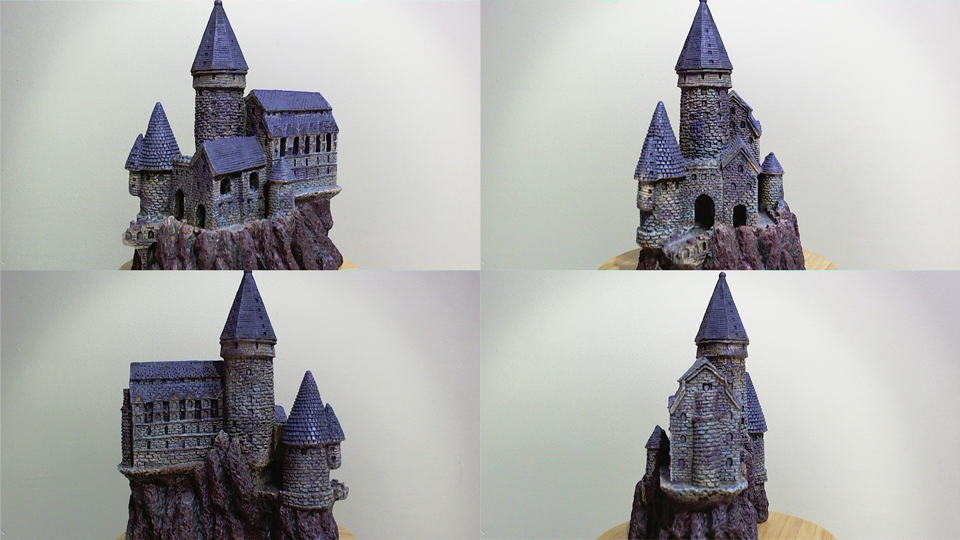
\includegraphics[width=1.0\textwidth]{images/castle.png}
\caption[R\'{e}plica miniatura de un castillo antiguo.]%
{R\'{e}plica miniatura de un castillo antiguo.}
\label{fig:ResultsCastle}
\end{figure}


El segundo objeto utilizado es una r\'{e}plica de unas columnas Griegas antiguas. En la figura ~\ref{fig:ResultsColumns} se muestran diferentes vistas de este objeto. Tiene un tama\~no aproximado de 17cm de alto, 21cm de ancho y 6cm de largo. Tambi\'{e}n se encuentra construido de un tipo de resina y est\'{a} pintado con diferentes tonos de caf\'{e} claro.


\begin{figure}[H]
\centering
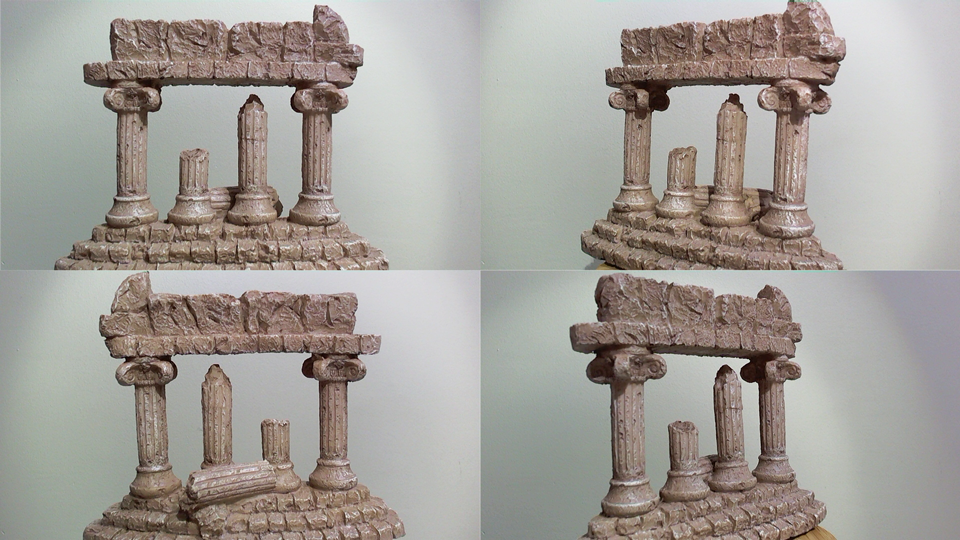
\includegraphics[width=1.0\textwidth]{images/greekcolumns.png}
\caption[R\'{e}plica miniatura de unas columnas Griegas]%
{R\'{e}plica miniatura de unas columnas Griegas.}
\label{fig:ResultsColumns}
\end{figure}

Se opt\'{o} por utilizar objetos cuya forma y color fueran considerablemente diferentes entre ellos con tal de observar el comportamiento del la t\'{e}cnica propuesta. A continuaci\'{o}n se muestran los resultados obtenidos a partir de un total de 300 reconstrucciones realizadas.


\section{Resoluci\'{o}n de im\'{a}genes vs. tiempo de reconstrucci\'{o}n}
Para la prueba se realiz\'{o} un total de 180 reconstrucciones (90 con el castillo y 90 con las columnas Griegas) utilizando la c\'{a}mara Logitech y un total de 120 reconstrucciones (60 con el castillo y 60 con las columnas Griegas) utilizando la c\'{a}mara Minoru. Se utilizaron tres diferentes resoluciones para la c\'{a}mara Logitech y dos para la c\'{a}mara Minoru. Por cada resoluci\'{o}n seleccionada se realizaron 30 reconstrucciones con ambas c\'{a}maras. Las resoluciones utilizadas fueron 640x480, 800x600 y 1024x768 para la c\'{a}mara Logitech mientras que para la c\'{a}mara Minoru se utiliz\'{o} \'{u}nicamente 640x480 y 800x600 debido a que no soporta 1024x768.

\begin{figure}[H]
\centering
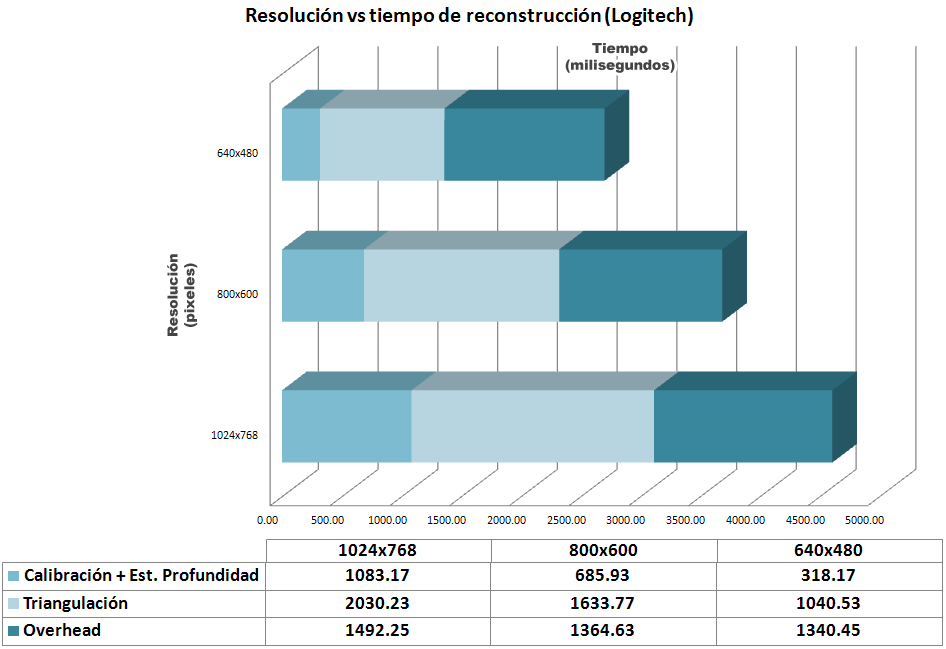
\includegraphics[width=1.0\textwidth]{images/chart-cl1.png}
\caption[Resoluci\'{o}n vs. tiempo de reconstrucci\'{o}n del castillo con la c\'{a}mara Logitech]%
{Resoluci\'{o}n vs. tiempo de reconstrucci\'{o}n del castillo con la c\'{a}mara Logitech. Los valores de tiempo est\'{a}n dados en milisegundos.}
\label{fig:ChartCL1}
\end{figure}


En la figura ~\ref{fig:ChartCL1} se muestran los resultados obtenidos a partir de 90 reconstrucciones realizadas al castillo desde todos los \'{a}ngulos posibles con la c\'{a}mara Logitech. La t\'{e}cnica se ejecut\'{o} 30 veces con capturas de 640x480 pixeles, 30 veces con capturas de 800x600 pixeles y finalmente, 30 veces con capturas de 1024x768 pixeles. La gr\'{a}fica muestra el promedio del tiempo total invertido (en milisegundos) en cada fase de la reconstrucci\'{o}n as\'{i} como el \textit{overhead} del experimento completo.


\begin{figure}[H]
\centering
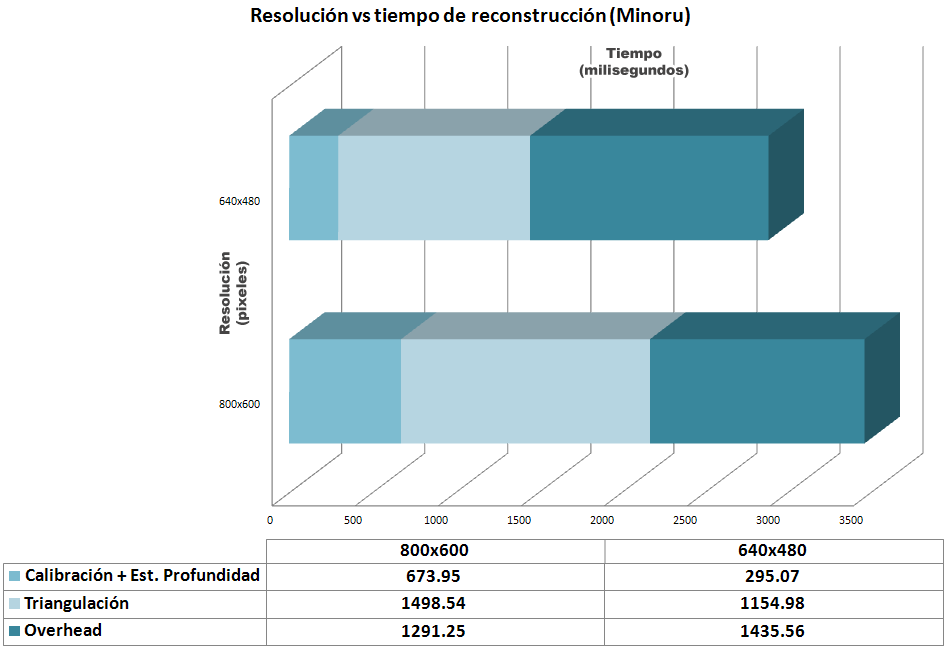
\includegraphics[width=1.0\textwidth]{images/chart-cm1.png}
\caption[Resoluci\'{o}n vs. tiempo de reconstrucci\'{o}n del castillo con la c\'{a}mara Minoru]%
{Resoluci\'{o}n vs. tiempo de reconstrucci\'{o}n del castillo con la c\'{a}mara Minoru. Los valores de tiempo est\'{a}n dados en milisegundos.}
\label{fig:ChartCM1}
\end{figure}


En la figura ~\ref{fig:ChartCM1} se muestran los resultados obtenidos a partir de 60 reconstrucciones realizadas al castillo desde todos los \'{a}ngulos posibles pero esta vez utilizando la c\'{a}mara Minoru. De igual forma, la t\'{e}cnica se ejecut\'{o} 30 veces con capturas de 640x480 pixeles y 30 veces con capturas de 800x600 pixeles. No fue posible ejecutarla con capturas de 1024x768 pixeles dado que la c\'{a}mara no soporta esa resoluci\'{o}n. La gr\'{a}fica muestra el promedio del tiempo total invertido (en milisegundos) en cada fase de la reconstrucci\'{o}n as\'{i} como el \textit{overhead} del experimento completo.


\begin{figure}[H]
\centering
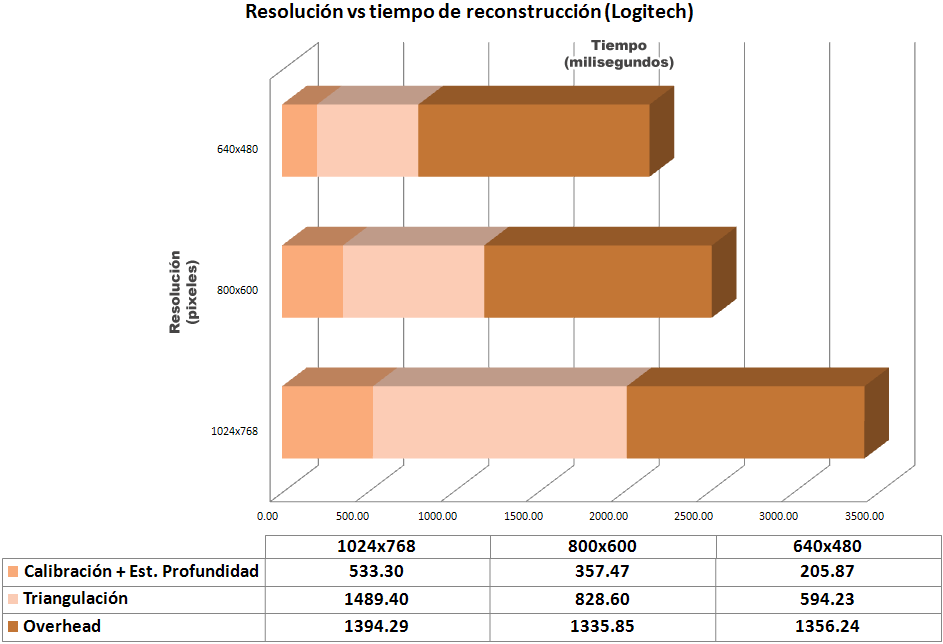
\includegraphics[width=1.0\textwidth]{images/chart-gl1.png}
\caption[Resoluci\'{o}n vs. tiempo de reconstrucci\'{o}n de las columnas Griegas con la c\'{a}mara Logitech]%
{Resoluci\'{o}n vs. tiempo de reconstrucci\'{o}n de las columnas Griegas con la c\'{a}mara Logitech. Los valores de tiempo est\'{a}n dados en milisegundos.}
\label{fig:ChartGL1}
\end{figure}


Seguidamente, se ejecut\'{o} la misma cantidad de reconstrucciones pero esta vez utilizando las columnas Griegas. En la figura ~\ref{fig:ChartGL1} se muestran los resultados obtenidos a partir de 90 reconstrucciones realizadas a las columnas desde todos los \'{a}ngulos posibles con la c\'{a}mara Logitech. Nuevamente, la t\'{e}cnica se ejecut\'{o} 30 veces con capturas de 640x480 pixeles, 30 veces con capturas de 800x600 pixeles y finalmente, 30 veces con capturas de 1024x768 pixeles.


\begin{figure}[H]
\centering
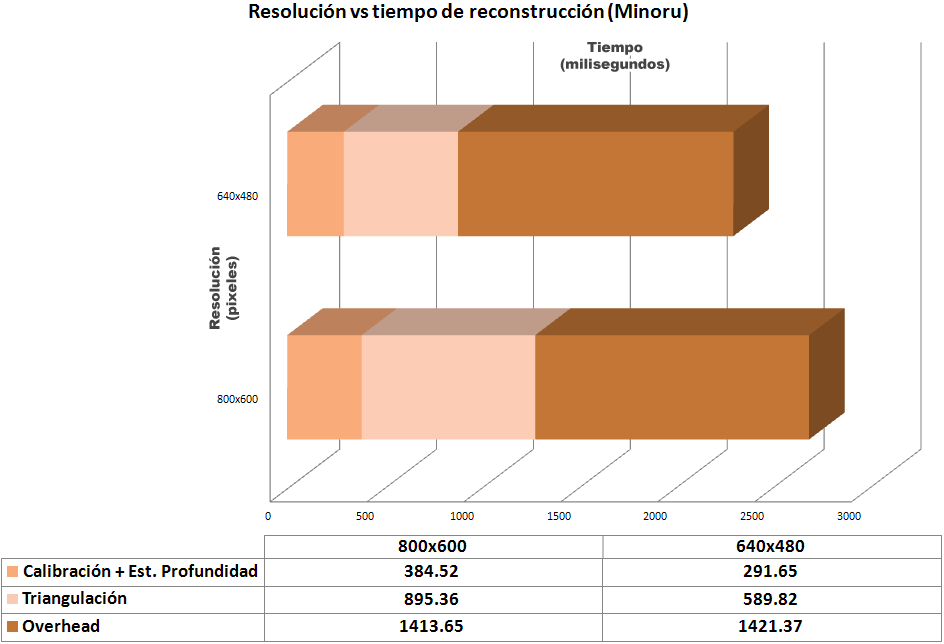
\includegraphics[width=1.0\textwidth]{images/chart-gm1.png}
\caption[Resoluci\'{o}n vs. tiempo de reconstrucci\'{o}n de las columnas Griegas con la c\'{a}mara Minoru]%
{Resoluci\'{o}n vs. tiempo de reconstrucci\'{o}n de las columnas Griegas con la c\'{a}mara Minoru. Los valores de tiempo est\'{a}n dados en milisegundos.}
\label{fig:ChartGM1}
\end{figure}


Finalmente, en la figura ~\ref{fig:ChartGM1} se muestran los resultados obtenidos a partir de las 60 reconstrucciones realizadas a las columnas desde todos los \'{a}ngulos posibles con la c\'{a}mara Minoru. De igual forma que con el castillo, la t\'{e}cnica se ejecut\'{o} 30 veces con capturas de 640x480 pixeles y 30 veces con capturas de 800x600 pixeles. No fue posible ejecutarla con capturas de 1024x768 pixeles debido a las limitaciones de la c\'{a}mara.


\section{Caracter\'{i}sticas f\'{i}sicas del objeto vs. tiempo de reconstrucci\'{o}n}
Para la prueba se utilizaron los mismos datos de las 300 reconstrucciones realizadas con ambas c\'{a}maras. Se utilizaron diferentes resoluciones para la c\'{a}mara Logitech y para la c\'{a}mara Minoru. Se contabiliz\'{o} el tiempo total de la reconstrucci\'{o}n y se promedi\'{o} la totalidad de los resultados para cada objeto.

\begin{figure}[H]
\centering
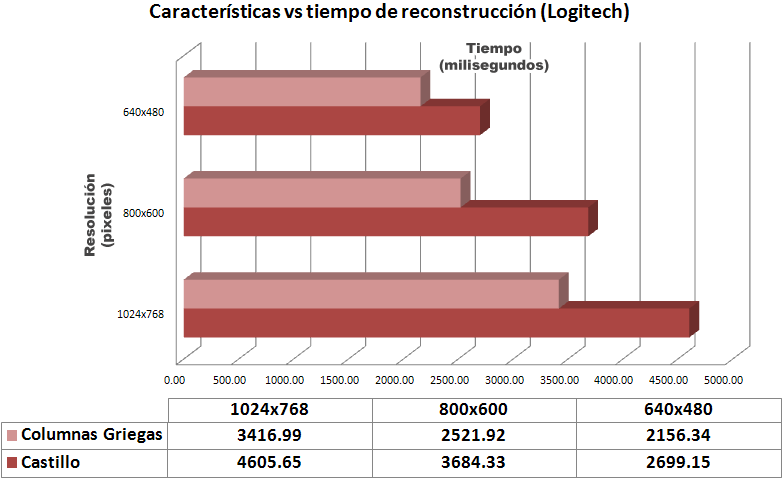
\includegraphics[width=1.0\textwidth]{images/featime1.png}
\caption[Caracter\'{i}sticas del objeto vs. tiempo de reconstrucci\'{o}n con la c\'{a}mara Logitech]%
{Caracter\'{i}sticas del objeto vs. tiempo de reconstrucci\'{o}n con la c\'{a}mara Logitech.}
\label{fig:FeatureVsTime1}
\end{figure}

En la figura ~\ref{fig:FeatureVsTime1} se muestran los resultados obtenidos con tres resoluciones 640x480, 800x600 y 1024x768 utilizando la c\'{a}mara Logitech con el castillo y las columnas Griegas.

\begin{figure}[H]
\centering
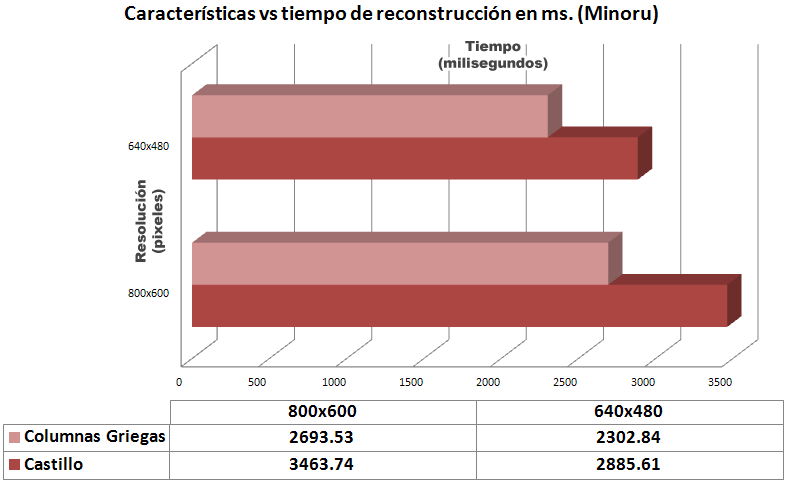
\includegraphics[width=1.0\textwidth]{images/featime2.png}
\caption[Caracter\'{i}sticas del objeto vs. tiempo de reconstrucci\'{o}n con la c\'{a}mara Minoru]%
{Caracter\'{i}sticas del objeto vs. tiempo de reconstrucci\'{o}n con la c\'{a}mara Minoru.}
\label{fig:FeatureVsTime2}
\end{figure}

Finalmente, en la figura ~\ref{fig:FeatureVsTime2} se muestran los resultados obtenidos para dos resoluciones 640x480 y 800x600 utilizando la c\'{a}mara Minoru nuevamente con el castillo y las columnas Griegas.


\section{Calibraci\'{o}n vs calidad de la reconstrucci\'{o}n}
Generalmente, cuando la calibraci\'{o}n falla los resultados obtenidos de la reconstrucci\'{o}n no se parecen en nada al objeto en cuesti\'{o}n. Fue necesario incorporar puntos de chequeo para determinar que los c\'{a}lculos obtenidos durante la fase de auto-calibraci\'{o}n (matrices \textit{P}) no sean totalmente err\'{o}neos. En la figura ~\ref{fig:WrongCalibration1} se muestra un ejemplo de una reconstrucci\'{o}n fallida del castillo por mala calibraci\'{o}n.

\begin{figure}[H]
\centering
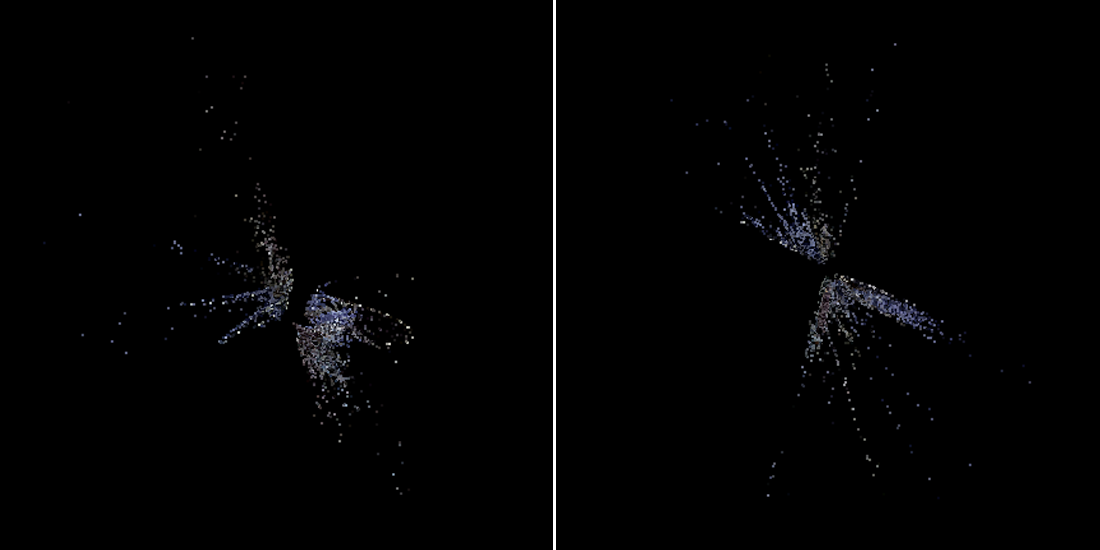
\includegraphics[width=1.0\textwidth]{images/wrongcal1.png}
\caption[Reconstrucci\'{o}n fallida del castillo]%
{Reconstrucci\'{o}n fallida del castillo. La imagen fue generada utilizando la t\'{e}cnica propuesta.}
\label{fig:WrongCalibration1}
\end{figure}

Otro ejemplo de reconstrucci\'{o}n fallida por mala calibraci\'{o}n se muestra en la figura ~\ref{fig:WrongCalibration2}. Esta vez, el objeto utilizado durante la reconstrucci\'{o}n fue el de las columnas Griegas.

\begin{figure}[H]
\centering
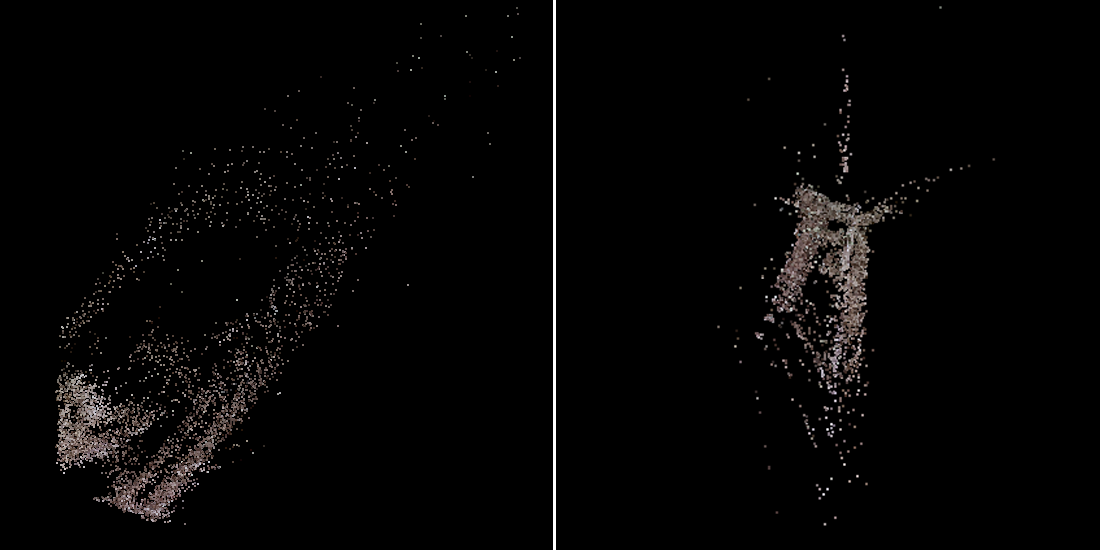
\includegraphics[width=1.0\textwidth]{images/wrongcal2.png}
\caption[Reconstrucci\'{o}n fallida de las columnas Griegas]%
{Reconstrucci\'{o}n fallida de las columnas Griegas. La imagen fue generada utilizando la t\'{e}cnica propuesta.}
\label{fig:WrongCalibration2}
\end{figure}

En la figura ~\ref{fig:CalibrationQuality} se muestra el porcentaje de fallos as\'{i} como la distribuci\'{o}n promedio en la calidad de las reconstrucciones obtenidas a partir de las 300 ejecuciones. Se le asign\'{o} un valor de 4 a una reconstrucci\'{o}n considerada como muy buena, 3 a una reconstrucci\'{o}n buena, 2 a una reconstrucci\'{o}n pobre y 1 a una reconstrucci\'{o}n mala (fallos).


\begin{figure}[H]
\centering
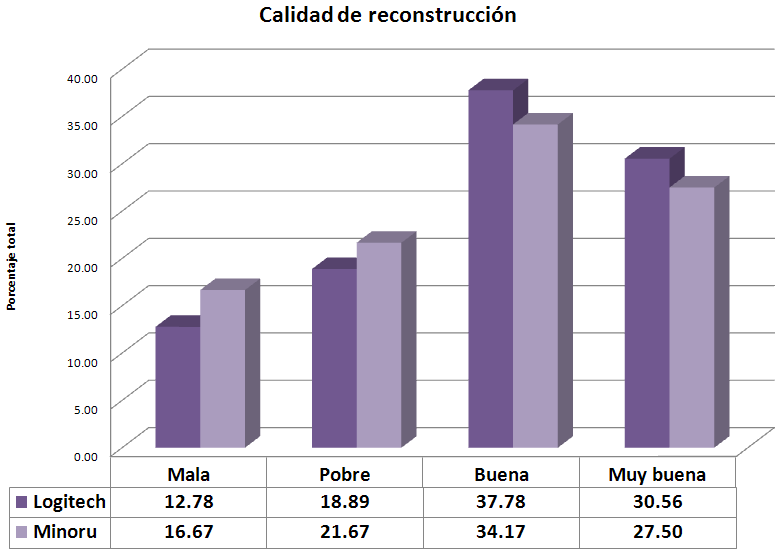
\includegraphics[width=1.0\textwidth]{images/calibquality1.png}
\caption[Calidad de la reconstrucci\'{o}n con ambas c\'{a}maras.]%
{Calidad de la reconstrucci\'{o}n con ambas c\'{a}maras.}
\label{fig:CalibrationQuality}
\end{figure}


Para efectos de comparaci\'{o}n se considera una reconstrucci\'{o}n mala cuando el resultado es totalmente incorrecto, como en el caso de las figuras ~\ref{fig:WrongCalibration1} y ~\ref{fig:WrongCalibration2}, una reconstrucci\'{o}n pobre cuando el resultado no es suficientemente denso y la distancia entre diferentes profundidades (por ej. las diferentes torres del castillo) no es cercana a la realidad del objeto, una reconstrucci\'{o}n buena cuando el resultado es denso y la distancia entre diferentes profundidades se asemeja m\'{a}s a la realidad del objeto. Finalmente, se considera una reconstrucci\'{o}n muy buena cuando los resultados son suficientemente densos y las m\'{e}tricas entre las diferentes profundidades son muy cercanas a la geometr\'{i}a real del objeto.


%A word of notice, many many times the reconstruction will fail because the Fundamental matrix came out wrong. The results will just look aweful, and nothing like a true reconstruction. To cope with this, you may want to insert a check that will make sure the two P matrices are not completely bogus (you could check for a reasonable rotation for example). If the P matrices, that are derived from the F matrix, are strange, then you can discard this F matrix and compute a new one.


\chapter{An\'{a}lisis de resultados}
\label{chap:analisis}
\epigraph{The falsification of scientific data or analysis is always a serious matter.}{Ed Markey}

En este cap\'{i}tulo se detalla el an\'{a}lisis de los resultados obtenidos durante las pruebas realizadas en la secci\'{o}n anterior as\'{i} como las relaciones encontradas a partir de esos datos.

\section{An\'{a}lisis}
De los resultados mostrados en las pruebas que eval\'{u}an la resoluci\'{o}n de las im\'{a}genes vs. el tiempo que toma la reconstrucci\'{o}n (figuras  ~\ref{fig:ChartCL1}, ~\ref{fig:ChartCM1}, ~\ref{fig:ChartGL1} y ~\ref{fig:ChartGM1}), se determin\'{o} que conforme la resoluci\'{o}n incrementa, el tiempo total de la reconstrucci\'{o}n incrementa. Con tal de ser m\'{a}s preciso en esta afirmaci\'{o}n se debe decir que a mayor cantidad de puntos detectados en las im\'{a}genes durante la fase de rastreo denso, mayor es el tiempo que toma procesarlos y por ende, mayor es el tiempo que toma la reconstrucci\'{o}n. La evidencia de esta relaci\'{o}n se nota m\'{a}s claramente en las figuras ~\ref{fig:FeatureVsTime1} y ~\ref{fig:FeatureVsTime2}, donde a pesar de utilizar una misma resoluci\'{o}n durante las pruebas, el tiempo de reconstrucci\'{o}n disminuye hasta en un 32\% en uno de los casos (resoluci\'{o}n a 800x600) debido a la diferencia geom\'{e}trica que existe entre los objetos reconstruidos. Particularmente y por sus espacios vac\'{i}os, las im\'{a}genes del objeto de las columnas Griegas generan una cantidad menor de puntos que las im\'{a}genes del castillo.

Se encontr\'{o} evidencia de que la calibraci\'{o}n influye considerablemente en la reconstrucci\'{o}n y por lo tanto, es considerada una de las fases m\'{a}s importantes de todo el proceso. Como se mencion\'{o} anteriormente, si la calibraci\'{o}n falla los resultados obtenidos al finalizar la reconstrucci\'{o}n ser\'{a}n err\'{o}neos y el resultado final no se parecer\'{a} en nada al objeto que se est\'{e} reconstruyendo, como se puede observar en las figuras ~\ref{fig:WrongCalibration1} y ~\ref{fig:WrongCalibration2}. Con tal de minimizar este problema se incorporaron puntos de chequeo para validar que los c\'{a}lculos obtenidos durante esta fase no sean completamente err\'{o}neos. Sin embargo, la incorporaci\'{o}n de estos puntos no garantiza que todas las reconstrucciones dar\'{a}n resultados satisfactorios. Factores como poca luz, detecci\'{o}n pobre del flujo \'{o}ptico, poco o mucho desplazamiento espacial entre im\'{a}genes, entre otros, tambi\'{e}n afectan la reconstrucci\'{o}n.

En la prueba que se muestra en la figura ~\ref{fig:CalibrationQuality}, el porcentaje de reconstrucciones fallidas se debi\'{o} a factores externos como los mencionados anteriormente y no a la c\'{a}mara ni al proceso de calibraci\'{o}n en s\'{i}. Uno de los factores que m\'{a}s afect\'{o} fue la diferencia de luz entre los pares de im\'{a}genes estereosc\'{o}picas debido a que la t\'{e}cnica no contempla controlar el auto-ajuste del foco ni el auto-balance de blancos de las c\'{a}maras durante las capturas.

No se encontr\'{o} evidencia que indique que la utilizaci\'{o}n de un tipo particular de c\'{a}mara (buena o mala calidad) afecta el proceso, la calidad o el tiempo de reconstrucci\'{o}n. De los resultados se desprende que la calidad de la reconstrucci\'{o}n no est\'{a} determinada por el tipo de c\'{a}mara que se utilice. Tambi\'{e}n se desprende que las diferencias encontradas en los tiempos de reconstrucci\'{o}n de las pruebas realizadas con la c\'{a}mara Logitech y la c\'{a}mara Minoru son despreciables en la mayor\'{i}a de los casos.

Finalmente, la hip\'{o}tesis que defiende esta tesis dice que \textbf{es posible reconstruir r\'{a}pidamente un objeto tridimensional a partir de, \'{u}nicamente, la informaci\'{o}n contenida en una secuencia de im\'{a}genes que provienen de una c\'{a}mara convencional de bajo costo y utilizando una serie de t\'{e}cnicas del campo de la visi\'{o}n artificial}. A pesar de las pruebas realizadas, no se encontró evidencia que indique lo contrario y por lo tanto, se asume cierta.

%\section{Modelo matem\'{a}tico}
%@TODO Torres??

%@TODO resumen del capitulo
\chapter{Conclusiones y trabajo futuro}
\label{chap:conclusiones}
\epigraph{The best way to predict the future is to implement it.}{Alan Curtis Kay}

En este cap\'{i}tulo se detalla las conclusiones del trabajo realizado as\'{i} como una secci\'{o}n de trabajo futuro.

\section{Conclusiones}
Esta tesis mostr\'{o} que es posible reconstruir r\'{a}pidamente un objeto tridimensional a partir de, \'{u}nicamente, la informaci\'{o}n contenida en una secuencia de im\'{a}genes provenientes de una c\'{a}mara convencional de bajo costo. Sin embargo, existen t\'{e}cnicas de reconstrucci\'{o}n mucho m\'{a}s robustas y complejas con las cuales es posible generar resultados de mayor calidad y precisi\'{o}n cuando el tiempo no es considerado un factor importante. 

Cabe destacar que a pesar de su simplicidad, la técnica propuesta genera resultados de gran calidad en un tiempo corto y sin la utilización de equipo especial. La principales conclusiones obtenidas a partir de este trabajo son:

\begin{itemize*}
\item No es necesario la utilizaci\'{o}n de equipo costoso especializado para lograr reconstrucciones tridimensionales de gran calidad.

\item La creaci\'{o}n de t\'{e}cnicas baratas de reconstrucci\'{o}n es necesaria debido a la gran demanda que existe por modelos tridimensionales de objetos f\'{i}sicos complejos.

\item La calidad de la c\'{a}mara utilizada para capturar las im\'{a}genes no es un factor determinante en la calidad de la reconstrucci\'{o}n final.

\item El proceso de calibraci\'{o}n de la c\'{a}mara es de suma importancia para lograr una reconstrucci\'{o}n tridimensional exitosa. En muchas ocasiones, la reconstrucci\'{o}n fallar\'{a} debido a que el c\'{a}lculo de la matriz fundamental \textit{F} fue err\'{o}neo, por lo que es necesario agregar tantas verificaciones como sea posible durante esta etapa para que la t\'{e}cnica de reconstrucci\'{o}n sea suficientemente robusta.

\item Utilizar t\'{e}cnicas pir\'{a}mide durante el procesamiento de las im\'{a}genes permite reducir la duraci\'{o}n de algoritmos de b\'{u}squeda de caracter\'{i}sticas sin necesidad de sacrificar informaci\'{o}n relevante para el proceso de reconstrucci\'{o}n tridimensional.

\item Algoritmos de flujo \'{o}ptico como el de Farnebäck y el de Lucas-Kanade pueden ser utilizados en reconstrucción r\'{a}pida y adem\'{a}s, permiten realizar una reconstrucci\'{o}n mucho m\'{a}s densa que si se realizara con algoritmos basados en caracter\'{i}sticas sobresalientes.
\end{itemize*}

\section{Trabajo futuro}
\textbf{Optimizaci\'{o}n}. Como trabajo futuro se puede optimizar el algoritmo para que tome ventaja de procesadores \textit{multicore} y así realizar muchos de los procesos de la t\'{e}cnica de forma paralela.

\textbf{Refinamiento}. Tambi\'{e}n se puede incorporar una etapa de refinamiento justo despu\'{e}s de la etapa de reconstrucci\'{o}n tridimensional de cada par de im\'{a}genes estereosc\'{o}picas con tal de mejorar la calidad de dicha reconstrucci\'{o}n. 

\textbf{Registro}. Adicionalmente, se puede implementar una etapa de registro posterior a la etapa de refinamiento con tal de poder realizar una reconstrucci\'{o}n completa de un objeto.

\textbf{Captura de vistas automatizado}. Finalmente, se puede implementar la automatizaci\'{o}n del proceso de captura de vistas con tal de minimizar la intervenci\'{o}n del usuario.

% Appendixes
\appendix 
\chapter{Ap\'{e}ndice}
\label{chap:apendice}

\section{Pseudoc\'{o}digo del algoritmo de reconstrucci\'{o}n 3D}
\begin{alltt}
\textbf{reconstructor_3d}
  \textbf{calibrar_camara}() \textit{// usar t\'{e}cnica del tablero de ajedrez}
    calcular la matriz de calibraci\'{o}n K
    calcular la matriz de distorsi\'{o}n D
  \textbf{fin}
  
  \textbf{capturar_vistas}() 
    \textit{// rotar objeto frente a la c\'{a}mara y capturar las vistas}
  \textbf{fin}
  
  \textbf{pareo_de_puntos}()
    \textbf{para} cada par de vistas KF1, KF2 \textbf{hacer en paralelo}
      detectar puntos clave para KF1, KF2 usando FAST con pir\'{a}mide
      calcular el flujo \'{o}ptico usando Farnebäck
      filtrar los puntos con alta tasa de error
      realizar un pareo de puntos entre KF1 y KF2 usando Brute-Force
    \textbf{fin}
  \textbf{fin}
  
  \textbf{eliminar_pareos_erroneos}()
    \textbf{para} cada par de vistas KF1, KF2 \textbf{hacer en paralelo}
      encontrar la matriz fundamental F para KF1 y KF2
      eliminar pareos erroneos usando F
    \textbf{fin}
  \textbf{fin}
  
  \textbf{calcular_matrices_de_camara}(KF1, KF2)
    calcular la matriz fundamental usando RANSAC
    calcular la matriz esencial (R,t) usando \(E = K'\sp{T}*F*K\)
  \textbf{fin}
  
  \textbf{triangular_puntos}(KF1, KF2)
    obtener matriz esencial para KF1 y KF2
    utilizar algoritmo de m\'{i}nimos cuadrados para la triangulaci\'{o}n
    retornar resultado de la triangulaci\'{o}n
  \textbf{fin}
  
  \textbf{encontrar_triangulacion_base}()
    // utilizar los pareos encontrados
    // reconstruir 2 vistas
    \textbf{para} cada par de pareos M1, M2 \textbf{hacer}
      obtener KF1, KF2 con M1, M2
      buena_matriz = calcular_matrices_de_camara(KF1, KF2);
      \textbf{si} buena_matriz = \textbf{true} \textbf{entonces}
        buena_triangulacion = triangular_puntos(KF1, KF2);
        \textbf{si} buena_triangulacion = \textbf{true} \textbf{entonces}
          agregar el calculo a la nube global de puntos
        \textbf{sino}
          buena_matriz = \textbf{false};
        \textbf{fin}
      \textbf{fin}
      \textbf{si} buena_matriz = \textbf{true} \textbf{entonces}
        salir del ciclo
      \textbf{fin}
    \textbf{fin}
  \textbf{fin}
  
  \textbf{recuperar_nueva_vista}()
    // realizar los mapeos 2D-3D
    // utilizar \textit{EPnP} con \textit{K} y mapeos para obtener nueva \textit{P1}
    // triangular usando nueva c\'{a}mara \textit{P1}
    // agregar nuevos puntos a la lista global
  \textbf{fin}

  \textbf{ejecutar}()
    calibrar_camara();
    capturar_vistas();
    pareo_de_puntos();
    eliminar_pareos_erroneos();
    encontrar_triangulacion_base();
    \textbf{para} cada nueva vista \textbf{hacer}
      recuperar_nueva_vista();
    \textbf{fin}
  \textbf{fin}
\textbf{fin}
\end{alltt}


% Final pages
\backmatter

% Use single space
\singlespacing

% Bibliography
\renewcommand{\bibname}{Referencias}
\cleardoublepage
\bibliographystyle{plainnat}
\refstepcounter{chapter}
\addcontentsline{toc}{chapter}{\bibname}
\bibliography{common/references.bib}

% Acronyms
\chapter{Acrónimos}

% Please keep it sorted by alphabetical order
\begin{acronym}

\acro{2D}{Bidimensional} es que posee dos dimensiones.

\acro{3D}{Tridimensional} es que posee tres dimensiones.

\acro{CCD}{Charge-Coupled Device} es un circuito integrado que contiene un número determinado de condensadores enlazados o acoplados. Bajo el control de un circuito interno, cada condensador puede transferir su carga eléctrica a uno o a varios de los condensadores que estén a su lado en el circuito impreso.

\acro{SIFT}{Scale Invariant Feature Transform} es un algoritmo de la visión artificial para detectar y describir características locales en imágenes. El algoritmo fue publicado por David Lowe en 1999 \cite{Lowe_1999}.

\acro{SURF}{Speeded Up Robust Feature} es un algoritmo robusto para la detección y descripción de características locales en imágenes creado por Herbert Bay et al. en el 2006. Basado parcialmente en \ac{SIFT} y según su autores, más rápido y robusto en las diferentes transformaciones de imágenes que \ac{SIFT} \cite{Bay_Ess_Tuytelaars_Vangool_2008}.

\acro{SLAM}{Simultaneous Localization And Mapping} es una t\'{e}cnica usada por robots y veh\'{i}culos aut\'{o}nomos para construir un mapa de un entorno desconocido en el que se encuentra, a la vez que estima su trayectoria al desplazarse dentro de este entorno.


\end{acronym}

\end{document}
